\documentclass[12pt, twocolumn]{article}
\setlength{\parindent}{0pt}
\usepackage[a4paper, top=1.5cm, bottom=2cm, left=1.5cm, right=1.5cm]{geometry}
\raggedbottom
\usepackage{amsmath,amssymb,dsfont}
\usepackage{graphicx} 
\usepackage{float}
\usepackage{bbold}
\usepackage{array}
\usepackage{hyperref}                  
\usepackage{enumitem} 
\usepackage{float}
\usepackage{setspace}
\usepackage{mathptmx}
\usepackage{titlesec}
\usepackage{fancyhdr}
\usepackage{lipsum} 
\usepackage{caption}
\usepackage{booktabs} 
\usepackage{threeparttable}
\usepackage{afterpage}
\usepackage{natbib}
\usepackage{stfloats}
\usepackage[section]{placeins}
\usepackage{balance}
\usepackage{stfloats}
\brokenpenalty=0 % Allow breaks in the current column
\usepackage{hyperref}

\clubpenalty=0      % Allow breaking after the first line of a paragraph
\widowpenalty=0     % Allow breaking before the last line of a paragraph
\displaywidowpenalty=0

% Customizing figure and table spacing
\setlength{\floatsep}{5pt}      % Space between floats
\setlength{\textfloatsep}{5pt}  % Space between float and text
\setlength{\intextsep}{5pt}     % Space between in-text float and text
\setlength{\abovecaptionskip}{0pt} % Space above captions
\setlength{\belowcaptionskip}{0pt} % Space below captions

% Customizing section, subsection, and paragraph spacing
\titleformat{\section}[block]{\large\bfseries}{\thesection.}{1em}{}
\titlespacing*{\section}{0pt}{10pt}{5pt} % {left}{before}{after}
\titleformat{\subsection}[block]{\normalsize\bfseries}{\thesubsection.}{1em}{}
\titlespacing*{\subsection}{0pt}{8pt}{4pt}

% Customizing paragraph spacing
\titleformat{\paragraph}[runin]{\normalsize\bfseries}{\theparagraph.}{1em}{}
\titlespacing*{\paragraph}{0pt}{6pt}{3pt} % {left}{before}{after}
\setlength{\parskip}{0pt}  % No extra spacing between paragraphs

% Redefining \normalsize to make sure it's in effect
\renewcommand{\normalsize}{\fontsize{10}{12}\selectfont} 
\normalsize

\captionsetup{font={normalsize, bf, rm}}

\fancypagestyle{plain}{
    \fancyhf{}
    \fancyfoot[L]{\textit{ISYE6420: Bayesian Data Analysis Project}}
    \fancyfoot[C]{\textit{}}
    \fancyfoot[R]{\thepage}
    \renewcommand{\footrulewidth}{0.001cm}
    \renewcommand{\headrulewidth}{0pt}
}
\pagestyle{plain} 

\title{\textbf{Bayesian Analysis in Flood Frequency Hydrology: \\ Verification with RMC-BestFit}}
\author{\textbf{Yanni Wang}}
\date{} 

\begin{document}
\maketitle
\pagestyle{fancy}


\begin{abstract}
This study investigates the application of Bayesian analysis in flood frequency hydrology, employing an adaptive Differential Evolution Markov Chain with Snooker Updater (DE-MCzS) algorithm for parameter estimation. The results were verified against BestFit, a state-of-the-art hydrological software developed by the U.S. Army Corps of Engineers Risk Management Center. Two case studies are presented: (1) a stationary flood frequency analysis of the Harricana River in Canada, which assesses the robustness of the Bayesian framework and its advantages over classical statistical methods, and (2) a non-stationary analysis of the O.C. Fisher Dam in the United States, examining temporal variability in flood frequency parameters. Through verification, we demonstrate the advantages of the Bayesian approach in terms of integrating uncertainty, accommodating temporal dynamics, and incorporating expert knowledge. By addressing challenges such as data limitations and evolving climatic conditions, it offers a robust framework for enhancing decision-making in hydrological risk management and infrastructure design.

\FloatBarrier
\end{abstract}

\section{Introduction}
Flood Frequency Analysis (FFA) is a fundamental aspect of hydrological studies, providing essential insights for the design of infrastructure, risk assessment, and water resource management. Accurate prediction of extreme flood events and their probabilities is critical for mitigating flood impacts, especially in regions vulnerable to climate variability and extreme weather events. Traditionally, statistical distributions for FFA have been estimated using Maximum Likelihood Estimation (MLE), which provides deterministic estimates based on available data. While effective, MLE does not inherently account for the uncertainties and variability often present in hydrological datasets, which limits its ability to fully represent the probabilistic nature of flood risks.

The Bayesian approach offers a robust alternative, providing a probabilistic framework that integrates uncertainty and prior knowledge into the analysis. By leveraging prior distributions and computing posterior probabilities, Bayesian methods enable hydrologists to quantify uncertainty in parameter estimates, yielding a more comprehensive understanding of flood risks. This capability is particularly valuable in hydrology, where data limitations and temporal variability in processes are common challenges. Additionally, Bayesian methods support the incorporation of expert judgment and allow for model updating as new data becomes available.

This study aims to provide a verification of the Bayesian computational framework implemented in BestFit, a software tool developed by the U.S. Army Corps of Engineers Risk Management Center (USACE RMC) to enhance and expedite advanced flood hazard assessments \citep{Smith_2020}. It has been widely used within the Flood Risk Management, Planning, and Dam and Levee Safety communities. Its latest release (version 2.0) in October 2024, introduces advanced capabilities for non-stationary FFA (NSFFA), enabling hydrologists to model temporal changes in flood frequency parameters \citep{Smith_2024}.

In the Bayesian estimation analysis, we employ the adaptive Differential Evolution Markov Chain with Snooker Updater (DE-MCzS) algorithm for the Markov Chain Monte Carlo (MCMC) process, as implemented in BestFit. Two case studies are presented to validate the computational framework: (1) a stationary analysis of the Harricana River in Canada, which compares the performance of the Bayesian approach against classical MLE, evaluates the DE-MCzS algorithm, and verifies posterior distributions with BestFit; and (2) both stationary and non-stationary FFA applied to the O.C. Fisher Dam in the United States, focusing on the verification of NSFFA with BestFit, comparison between stationary and non-stationary models, and examining the influence of temporal variability on flood frequency curves.

\FloatBarrier


\section{Data}
This study utilizes two publicly available datasets for validation and analysis. The first dataset is the Harricana River at Amos (Quebec, Canada), sourced from \citep{Bobee_1991, Smith_2020b}. The dataset, comprising observed annual flow peak data, is detailed in Appendix A. The second dataset corresponds to the O.C. Fisher Dam, located on the North Concho River in Texas. This dataset is provided in the documentation accompanying the latest release of RMC-BestFit \citep{Smith_2024}. The data is presented in Appendix B.

\FloatBarrier


\section{Methodology}
\subsection{Statistical Concepts in Flood Frequency Hydrology}
Flood frequency hydrology involves fitting statistical distributions to annual flood peak data to model their probabilistic behavior. Frequency curves are then derived using Z-score transformations, which enables consistent interpretation of extreme event probabilities across different datasets. 

\subsubsection{Log-Pearson Type III (LP3) Distribution}
Among various statistical distributions, the Log-Pearson Type III (LP3) distribution is widely adopted for its ability to model the skewness inherent in annual flood peak data \citep{Singh_1998}. Let $Y$ represent independent and identically distributed (i.i.d) annual flood peak discharges:
$$Y = \{y_i \mid i = 1, 2, ..., n\}$$
 
Applying a logarithmic transformation:
$$x_i = \log_{10} (y_i)$$

The transformed data $x_i$ follows a Pearson Type III distribution, which is parametrized using its moments: the mean ($\mu$), standard deviation ($\sigma$) and skew ($\gamma$). The corresponding true parameters - location ($\xi$), shape ($\alpha$) and scale ($\beta$) - are computed as: 
\begin{align*}
    \xi = \mu - \frac{2 \sigma}{\gamma}, \quad \alpha = \frac{4}{\gamma^2}, \quad \beta = 0.5 \sigma \gamma 
\end{align*}

The probability density function (PDF) of the LP3 distribution is given by:
$$f_{\text{LP3}}(y_i \mid \mu, \sigma, \gamma) = f_{\text{gamma}} (x_i - \xi; \alpha, \beta) \cdot J$$
where $f_{\text{gamma}}$ denotes the gamma distribution, and $J$ is the Jacobian determinant:
$$J = \bigg| \frac{\partial (y_i)}{\partial x_i} \bigg|  = \bigg| \frac{\partial \log_{10} (y_i)}{\partial y_i} \bigg| = \frac{1}{y_i \cdot \ln(10)}$$

\subsubsection{Z-scores Transformation}
\label{sec:z_scores}
In hydrology, the Annual Exceedance Probability (AEP) is usually used to describe the likelihood of extreme events. It is defined as he probability that a particular hydrological event will be equaled or exceeded in any given year:
$$\text{AEP} = 1 -q$$
where $q$ is the cumulative probability associated with the quantile. For example, a quantile $q=0.99$ corresponds to an AEP of 1\%, meaning there’s a 1\% chance that the event magnitude will be exceeded.

Z-scores are used to standardize event probabilities. The Z-score represents the number of standard deviations by which a value lies from the mean in a standard normal distribution. For a given quantile $q$, the Z-score is calculated as:
$$Z(q) = -\Phi^{-1}(1-q) = -\Phi^{-1}(\text{AEP})$$
where $\Phi^{-1}$ is the Percent Point Function (PPF), or the inverse of the Cumulative Distribution Function (CDF) of the standard normal distribution.

\subsection{Maximum Likelihood Estimation (MLE)}
In the classical approach, the parameters of distributions ($\mu$, $\sigma$ and $\gamma$ for LP3) are estimated using the Maximum Likelihood Estimation (MLE) method. The likelihood function represents the probability of observing the data, $Y =(y_1, y_2,..., y_n)$, conditional on the distribution parameters: 
$$L (Y \mid \mu, \sigma, \gamma) =\prod_{i=1}^n f_{\text{LP3}} (y_i \mid \mu, \sigma, \gamma)$$

The natural logarithm of the likelihood simplifies the computation: 
$$\log L (Y \mid \mu, \sigma, \gamma) =\sum_{i=1}^n \big[\log f_{\text{gamma}} (x_i - \xi; \alpha, \beta) - \log \big(y_i \cdot \ln(10) \big) \big]$$

The parameters are estimated by minimizing the negative log-likelihood, a process that converts the maximization of the likelihood function into a minimization problem. The Nelder-Mead optimization method is employed for this purpose, ensuring efficient and robust estimation of the LP3 parameters.

\subsection{Bayesian Estimation Analysis}
In Bayesian analysis, parameter uncertainties are quantified through prior distributions  $\pi(\theta)$, where $\theta = \{\mu, \sigma, \gamma\}$ for LP3. Combining these priors with the likelihood function, $L (Y \mid \theta)$, derived from the observed data, the posterior distribution is:
$$ \pi (\theta \mid Y) = \frac{L (Y \mid \theta) \pi(\theta)}{\int L (Y \mid \theta) \pi(\theta) d\theta}$$
Since the integral in the denominator is generally intractable, Markov Chain Monte Carlo (MCMC) methods are used to approximate the posterior distribution through iterative sampling. To efficiently explore the parameter space and overcome potential convergence issues, we implement an adaptive Differential Evolution Markov Chain with Snooker updater (DE-MCzS) algorithm, as utilized in the BestFit software. The schematic diagram of the Bayesian framework is illustrated in Figure \ref{fig:DE-MCzS}. 

Unlike traditional MCMC methods that rely on a single chain, differential evolution markov chains maintain a population of chains that evolve collectively. This population-based approach allows chains to share information with candidate proposals informed by the states of other chains, thereby enhancing the algorithm's ability to navigate complex posterior landscapes. The DE-MCzS algorithm incorporates a snooker updater to further improve mixing and avoid local convergence traps \citep{Cheng_2014, Cheng_2014_b, Braak_2018}. The snooker updater generates proposals orthogonal to the chain's current trajectory. It leverages line projections to focus exploration on less-visited regions of the parameter space. The combination of differential evolution strategies and adaptive updates makes DE-MCzS effective and robust in Bayesian inference problems that are high-dimensional or involve multimodal distributions.

\begin{figure*}[ht!]
    \centering
    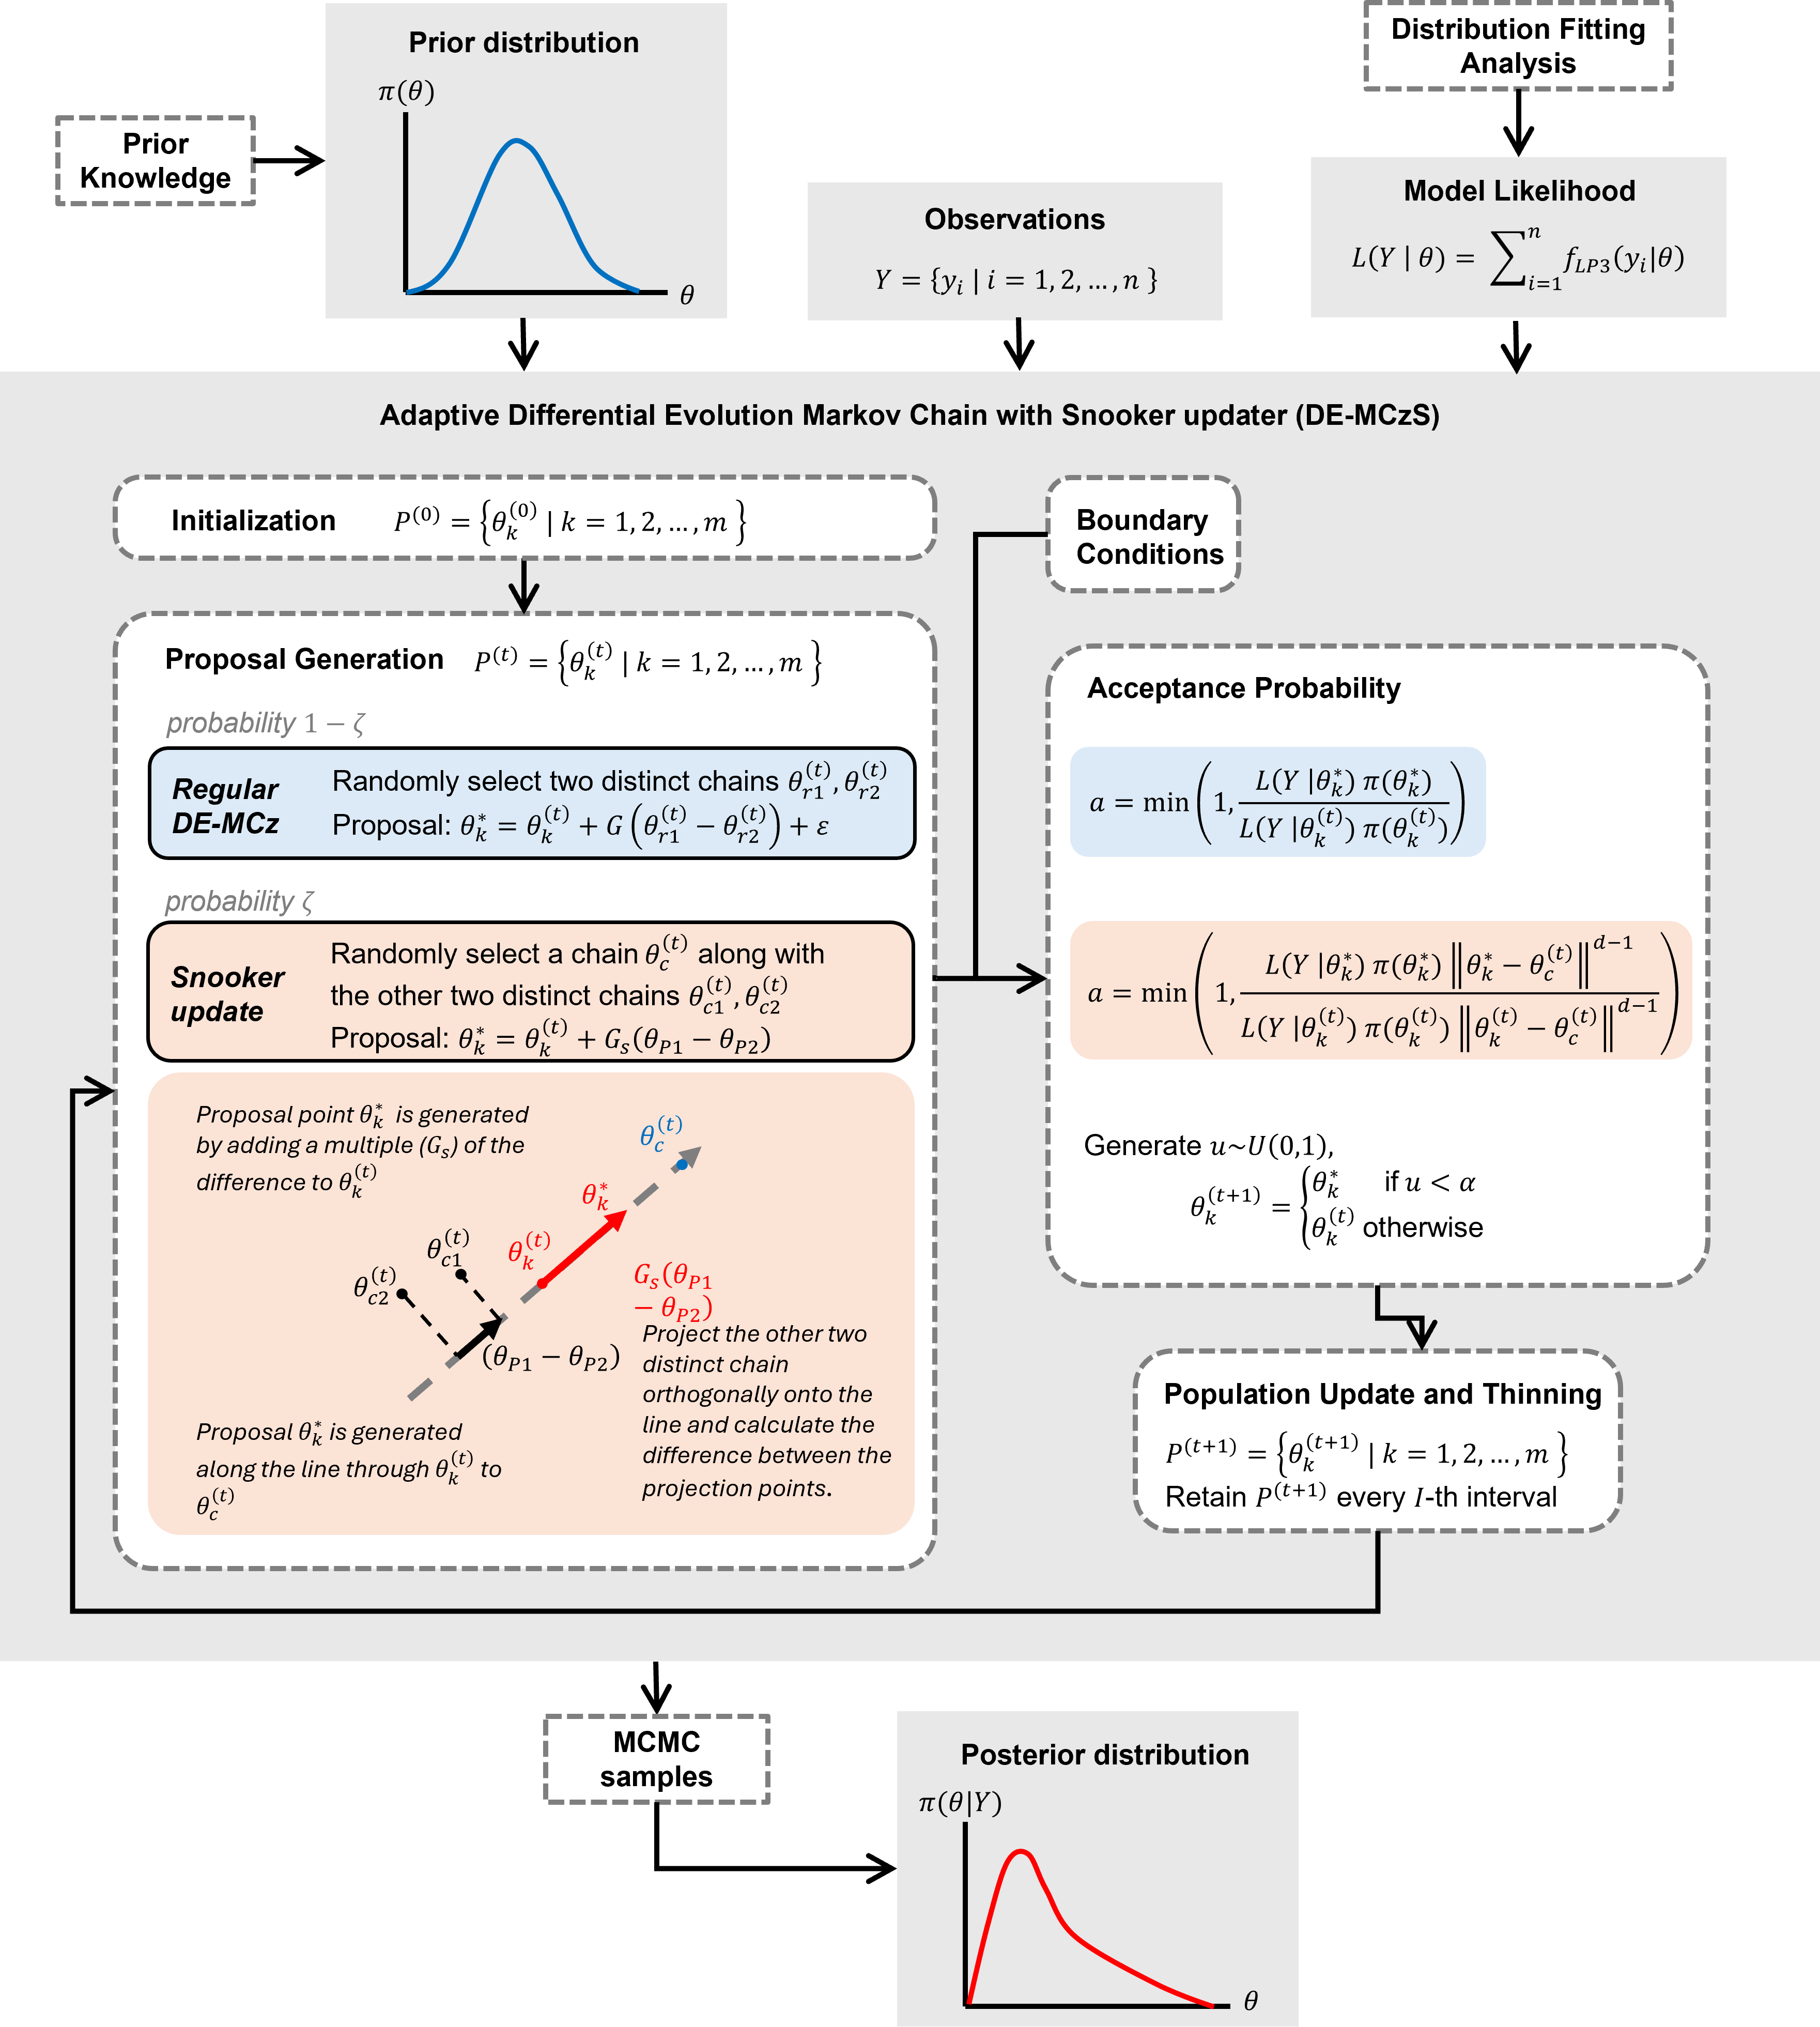
\includegraphics[width=1\linewidth]{_plots/DE-MCzS.png}
    \caption{Schematic representation of the Adaptive Differential Evolution Markov Chain with Snooker Update (DE-MCzS) algorithm. The diagram illustrates the Bayesian framework, including the prior distribution $\pi(\theta)$, the likelihood function $L(Y \mid \theta)$, and the posterior distribution $\pi(\theta \mid Y)$. Key steps of the algorithm are shown, such as initialization, proposal generation (regular and snooker updates), acceptance probability calculation, and posterior sampling.}
    \label{fig:DE-MCzS}
\end{figure*}

\subsubsection{Adaptive Differential Evolution Markov Chain with Snooker updater (DE-MCzS)}
\paragraph{Initialization}
The algorithm begins by initializing a population $P^{(0)}$ of $m$ chains, each containing a parameter vector $\theta_k^{(0)}$ sampled from the prior distribution:
$$P^{(0)} = \{{\theta_k}^{(0)}\mid k =1,2, ...,m\}$$

\paragraph{Proposal Generation} 
At iteration $t$, chain $k$ generates a proposal $\theta_k^*$, either through a regular DE-MCz update, or snooker update with a specified probability $\zeta$ (commonly set to $0.1$).

\paragraph{Regular DE-MCz Update}
The differential evolution strategy generates proposals by randomly selecting two distinct chains, $\theta_{r1}^{(t)}$ and $\theta_{r2}^{(t)}$ , and computing:
$$\theta_k^* = \theta_k^{(t)} + G\big( \theta_{r1}^{(t)} -\theta_{r2}^{(t)} \big) + \epsilon$$
where $G$ is a scaling factor and $\epsilon$ is a small perturbation term to maintain ergodicity and avoid premature convergence.

The scaling factor $G$ is determined based on a probability threshold $\delta$ and the jump parameter $\gamma$, as follows:
$$G = \begin{cases} 
1, & \text{with probability } \delta \\ 
\gamma, & \text{with probability } (1 - \delta) 
\end{cases}$$
where $\delta$ is typically set to $0.1$, and $\gamma$ is calculated as $\gamma = \frac{2.38}{\sqrt{2j}}$, with $j$ being the dimensionality of the parameter vector $\theta$. 

In BestFit, the perturbation $\epsilon$ is generated using a PPF-based noise term with power transformation:
$$\epsilon = (\Phi^{-1}(U))^p$$
where $\Phi^{-1}$ is the PPF (inverse CDF) of the standard normal distribution, $U \sim \text{Uniform} (0, 1)$, and $p$ is the exponent representing the number of parameters.
In this study, however, we adopt the Gaussian noise term for  $\epsilon$:
$$\epsilon \sim N(0, \sigma^2I)$$
where $I$ is the identity matrix, and $\sigma^2$ is the variance which is typically set to a small value such as $10^{-3}$.

\paragraph{Snooker Update}
In the snooker update, a chain $\theta_c^{(t)}$ is selected at random from the population. 
The proposal is generated along the line through $\theta_k^{(t)}$ to $\theta_{c}^{(t)}$, which is defined as:
$$\mathbf{l} = \theta_k^{(t)} - \theta_{c}^{(t)}$$
and its squared norm is:
$${\parallel\mathbf{l}\parallel}^2 = \mathbf{l}^\top \mathbf{l}$$
Two additional chains, $\theta_{c1}^{(t)}$ and $\theta_{c2}^{(t)}$, are selected, and their orthogonal projections onto the line $\mathbf{l}$ are calculated as:
$$\theta_{P1} = \theta_{c}^{(t)} + \frac{(\theta_{c1}^{(t)} - \theta_{c}^{(t)})^\top \mathbf{l}}{{\parallel\mathbf{l}\parallel}^2}\mathbf{l}, \quad \theta_{P2} = \theta_{c}^{(t)} + \frac{(\theta_{c2}^{(t)} - \theta_{c}^{(t)})^\top \mathbf{l}}{{\parallel\mathbf{l}\parallel}^2}\mathbf{l}$$
The proposal is then generated along the line $\mathbf{l}$ as:
$$\theta_k^* = \theta_k^{(t)} + G_s( \theta_{P1} - \theta_{P2})$$
where $G_s$ is a snooker-specific scaling factor sampled from a uniform distribution, typically $G_s \sim \text{Uniform}(1.2, 2.2)$.


\paragraph{Boundary Conditions}
Any proposed parameter vector $\theta_k^*$ that falls outside the feasible bounds defined by the prior distributions is automatically rejected to ensure the validity of the samples.

\paragraph{Acceptance Probability}
The acceptance of the proposed parameter vector $\theta_k^*$ is determined using the Metropolis-Hastings criterion. For the regular DE-MCz update, the acceptance probability $\alpha$ is calculated as:

$$a = \min \bigg(1, \frac{L(Y \mid \theta_k^*) \cdot \pi(\theta_k^*)}{L(Y \mid \theta_k^{(t)}) \cdot \pi(\theta_k^{(t)})}\bigg)$$

For the snooker update, the acceptance probability accounts for the change in volume due to the move being along a line, and is given by:
$$a = \min \bigg(1, \frac{L(Y \mid \theta_k^*) \cdot \pi(\theta_k^*) \cdot \parallel \theta_k^* - \theta_c^{(t)}\parallel ^{d-1}}{L(Y \mid \theta_k^{(t)}) \cdot \pi(\theta_k^{(t)}) \cdot \parallel \theta_k^{(t)} - \theta_c^{(t)}\parallel ^{d-1}}\bigg)$$
where $d$ is the dimensionality of the parameter space.

A uniform random number $u \sim \text{Uniform}(0, 1)$ is generated, and the chain is updated as:
$$\theta_k^{(t+1)} = 
\begin{cases} 
\theta_k^*, & \text{if } u < \alpha\\ 
\theta_k^{(t)}, & \text{otherwise} 
\end{cases}$$

\paragraph{Population Update and Thinning}
After all chains have been updated, the population becomes:
$$P^{(t+1)} = \{ \theta_k^{(t+1)}\mid k =1,2, ...,m\}$$
This updated population serves as the starting point for the next iteration. 

To reduce autocorrelation and improve statistical properties of MCMC samples, thinning is applied by retaining every $I$-th iteration:
$$\text{Retain sample at iteration } t \text{ if }t = zI, \quad z \in \mathbb{Z}^+$$
Additionally, an initial burn-in period is discarded to allow the chains to converge to the target distribution. At the conclusion of the simulation, a total of $N = 10,000$ samples are stored as the MCMC samples, which provides a comprehensive representation of the posterior distribution.

\subsubsection{Posterior Mode}
The posterior mode identifies the parameter values $\theta_{\text{mode}}$ that maximize the posterior probability density:
$$\theta_{\text{mode}} = \arg\max_{\theta} \pi(\theta \mid Y)$$

To simplify computations, the log-posterior is typically maximized instead:
$$\log \pi(\theta \mid Y) = \log L(Y \mid \theta) + \log \pi(\theta)$$

In cases where the prior distribution $\pi(\theta )$ is uniform or weakly informative, $\log \pi(\theta)$ becomes constant or negligible. As a result, the computation reduces to maximizing the log-likelihood:
$$\theta_{\text{mode}} = \arg\max_{\theta} \log L(Y\mid \theta)$$

Once $\theta_{\text{mode}}$ is computed, the posterior mode for a given quantile $q$ is calculated using the PPF:
$$\big\{F^{-1} (q_j \mid \theta_{\text{mode}}) \mid j = 1, 2, ..., M\big\}$$
where $F^{-1}$ is the PPF (inverse CDF) of the LP3 distribution, and $q_j$ represents the desired quantile value for $M$ quantiles of interest.

\subsubsection{Posterior Predictive and Credible Intervals}
The posterior predictive distribution evaluates the probability of future observations $\tilde{Y}$, conditioned on the observed data $Y$. This distribution accounts for both uncertainty in parameter estimates and variability in the data: 
$$\pi (\tilde{Y} \mid Y)= \int \pi(\tilde{Y} \mid \theta)\pi(\theta\mid Y) d\theta$$

Due to the intractability of this integral, the posterior predictive distribution is usually approximated through sampling. A logarithmic binning approach is adopted, as employed in BestFit, to efficiently capture a wide range of predictive values.

For each desired quantile $q_j$, PPF is computed for posterior samples $\theta^{(s)}$ obtained from MCMC samples: 
$$\big\{F^{-1} (q_j \mid \theta^{(s)}) \mid j = 1, 2, ..., M\big\}$$

The PPF values for all quantiles are transformed to the logarithmic scale. This range is divided into $B = 20$ bins using the minimum and maximum values:
$$\text{min PPF} = \log \big(\min \big\{F^{-1} (q_j \mid \theta^{(s)} ) \mid j = 1, 2, ...M \big\}\big)$$
$$\text{max PPF} = \log \big(\max \big\{F^{-1} (q_j \mid \theta^{(s)}) \mid j = 1, 2, ...M \big\}\big)$$

The bin edges represent future observations $\tilde{Y}$:
$$ \{\tilde{Y}\} = \big\{ \text{min PPF}, \text{min PPF}+ 10^{\frac{\text{max PPF} - \text{min PPF}}{B-1}}, ..., \text{max PPF} \big\}$$

For each bin $\tilde{Y}$, the CDF is used to compute the probability that $Y$ takes a value less than or equal to $\tilde{Y}$, given each sampled parameter set $\theta^{(s)}$. The averaged value across all samples is:
$$q({\tilde{Y}}) = \frac{1}{N} \sum_{s=1}^N F(\tilde{Y} \mid \theta^{(s)})$$
where $F$ is the CDF of the LP3 distribution. This quantile $q({\tilde{Y}})$ can be transformed into Z-scores $Z({\tilde{Y}})$ as describes in Section \ref{sec:z_scores}. 

Once Z-scores are computed for all bins, interpolation is used to estimate posterior predictive values for each desired quantile $q_j$:
$$\big \{\text{Interp} \big(Z(q_j)), \{Z({\tilde{Y}})\}, \{\tilde{Y}\}\big) \mid j = 1, 2, ..., M \big\}$$

For each quantile, credible intervals are numerically determined from the sampled PPF values. To construct a $(1 - 2a) \times 100\%$ credible interval, the bounds are defined as::
$$\text{Lower bound}: \text{Percentile} \big(a \cdot 100 \big)$$
$$\text{Upper bound}: \text{Percentile} \big((1-a) \cdot 100 \big)$$

\subsection{Non-stationarity}
\label{sec:nsffa}
In the Bayesian FFA described earlier, the observed data $Y = \{y_i \mid i = 1, 2, ..., n\}$ is assumed to be independent and identically distributed
(i.i.d). However, this assumption may not hold true in a non-stationary environment, particularly under the influence of climate change. Non-stationary flood frequency analysis (NSFFA) accounts for temporal variations in the parameter vectors $\theta$, resulting in a time-dependent likelihood function \citep{Smith_2024}:
$$L (Y \mid \theta) =\prod_{t=1}^T f_{\text{LP3}} (y_i \mid \theta_t)$$
where $\theta_t$ is the parameter set for time step $t$, which allows the distribution to evolve over time.

In this study, non-stationarity is considered only with respect to the location parameter $\mu$, as temporal variations in the scale parameter $\sigma$  and shape parameter $\gamma$ require substantial long-term data, which is often difficult to obtain \citep{Cheng_2014_b}. Temporal changes in $\mu$ are modeled using linear and exponential trends:
\begin{align*}
    \text{linear: } & \mu_t = \beta_0 + \beta_1 \cdot t\\
    \text{exponential: } & \mu_t = \beta_0 \cdot \exp (\beta_1 \cdot t)
\end{align*}
where $t$ is the time in years (with $t=0$ representing the first observed data point), $\beta_0$ is the intercept representing the initial location parameter at $t=0$, and $\beta_1$ is the coefficient controlling the strength of the trend over time. 

In NSFFA, each time step has a unique parameter set, which means there is a unique set of distribution properties over time. As a result, the exceedance probabilities of flow values also varies with time. A time index property is introduced in BestFit to determine the time step for evaluating the non-stationary frequency distribution \citep{Smith_2024}. 

\FloatBarrier
 

\section{Results and Discussion}

\subsection{Case study 1: Harricana River, Canada}
The Harricana River dataset firstly provides a basis for comparing traditional MLE with the Bayesian approach for FFA. Using the MLE method, the LP3 distribution was fitted to estimate parameters using the Nelder-Mead
optimization algorithm (Figure \ref{fig:HRA_LP3_MLE}), which produces a single deterministic flood frequency curve, as shown in Figure \ref{fig:HRA_flood_quantiles_MLE}. 

In contrast, the Bayesian approach allows for the incorporation of prior distributions and explicit modeling of parameter uncertainty. A stationary FFA was conducted in this case study, with a rigorous evaluation of the adaptive DE-MCzS algorithm and verification of posterior distributions with BestFit. The stationary FFA model assumes the following uniform priors:
\begin{align*}
    Y \mid \mu, \sigma, \gamma &\sim \text{LP3}(\mu, \sigma, \gamma)\\
    \mu &\sim \text{Uniform}(0,4)\\
    \sigma &\sim \text{Uniform}(0,2)\\
    \gamma &\sim \text{Uniform}(-2,2)
\end{align*}

\begin{figure}[ht!]
    \centering
    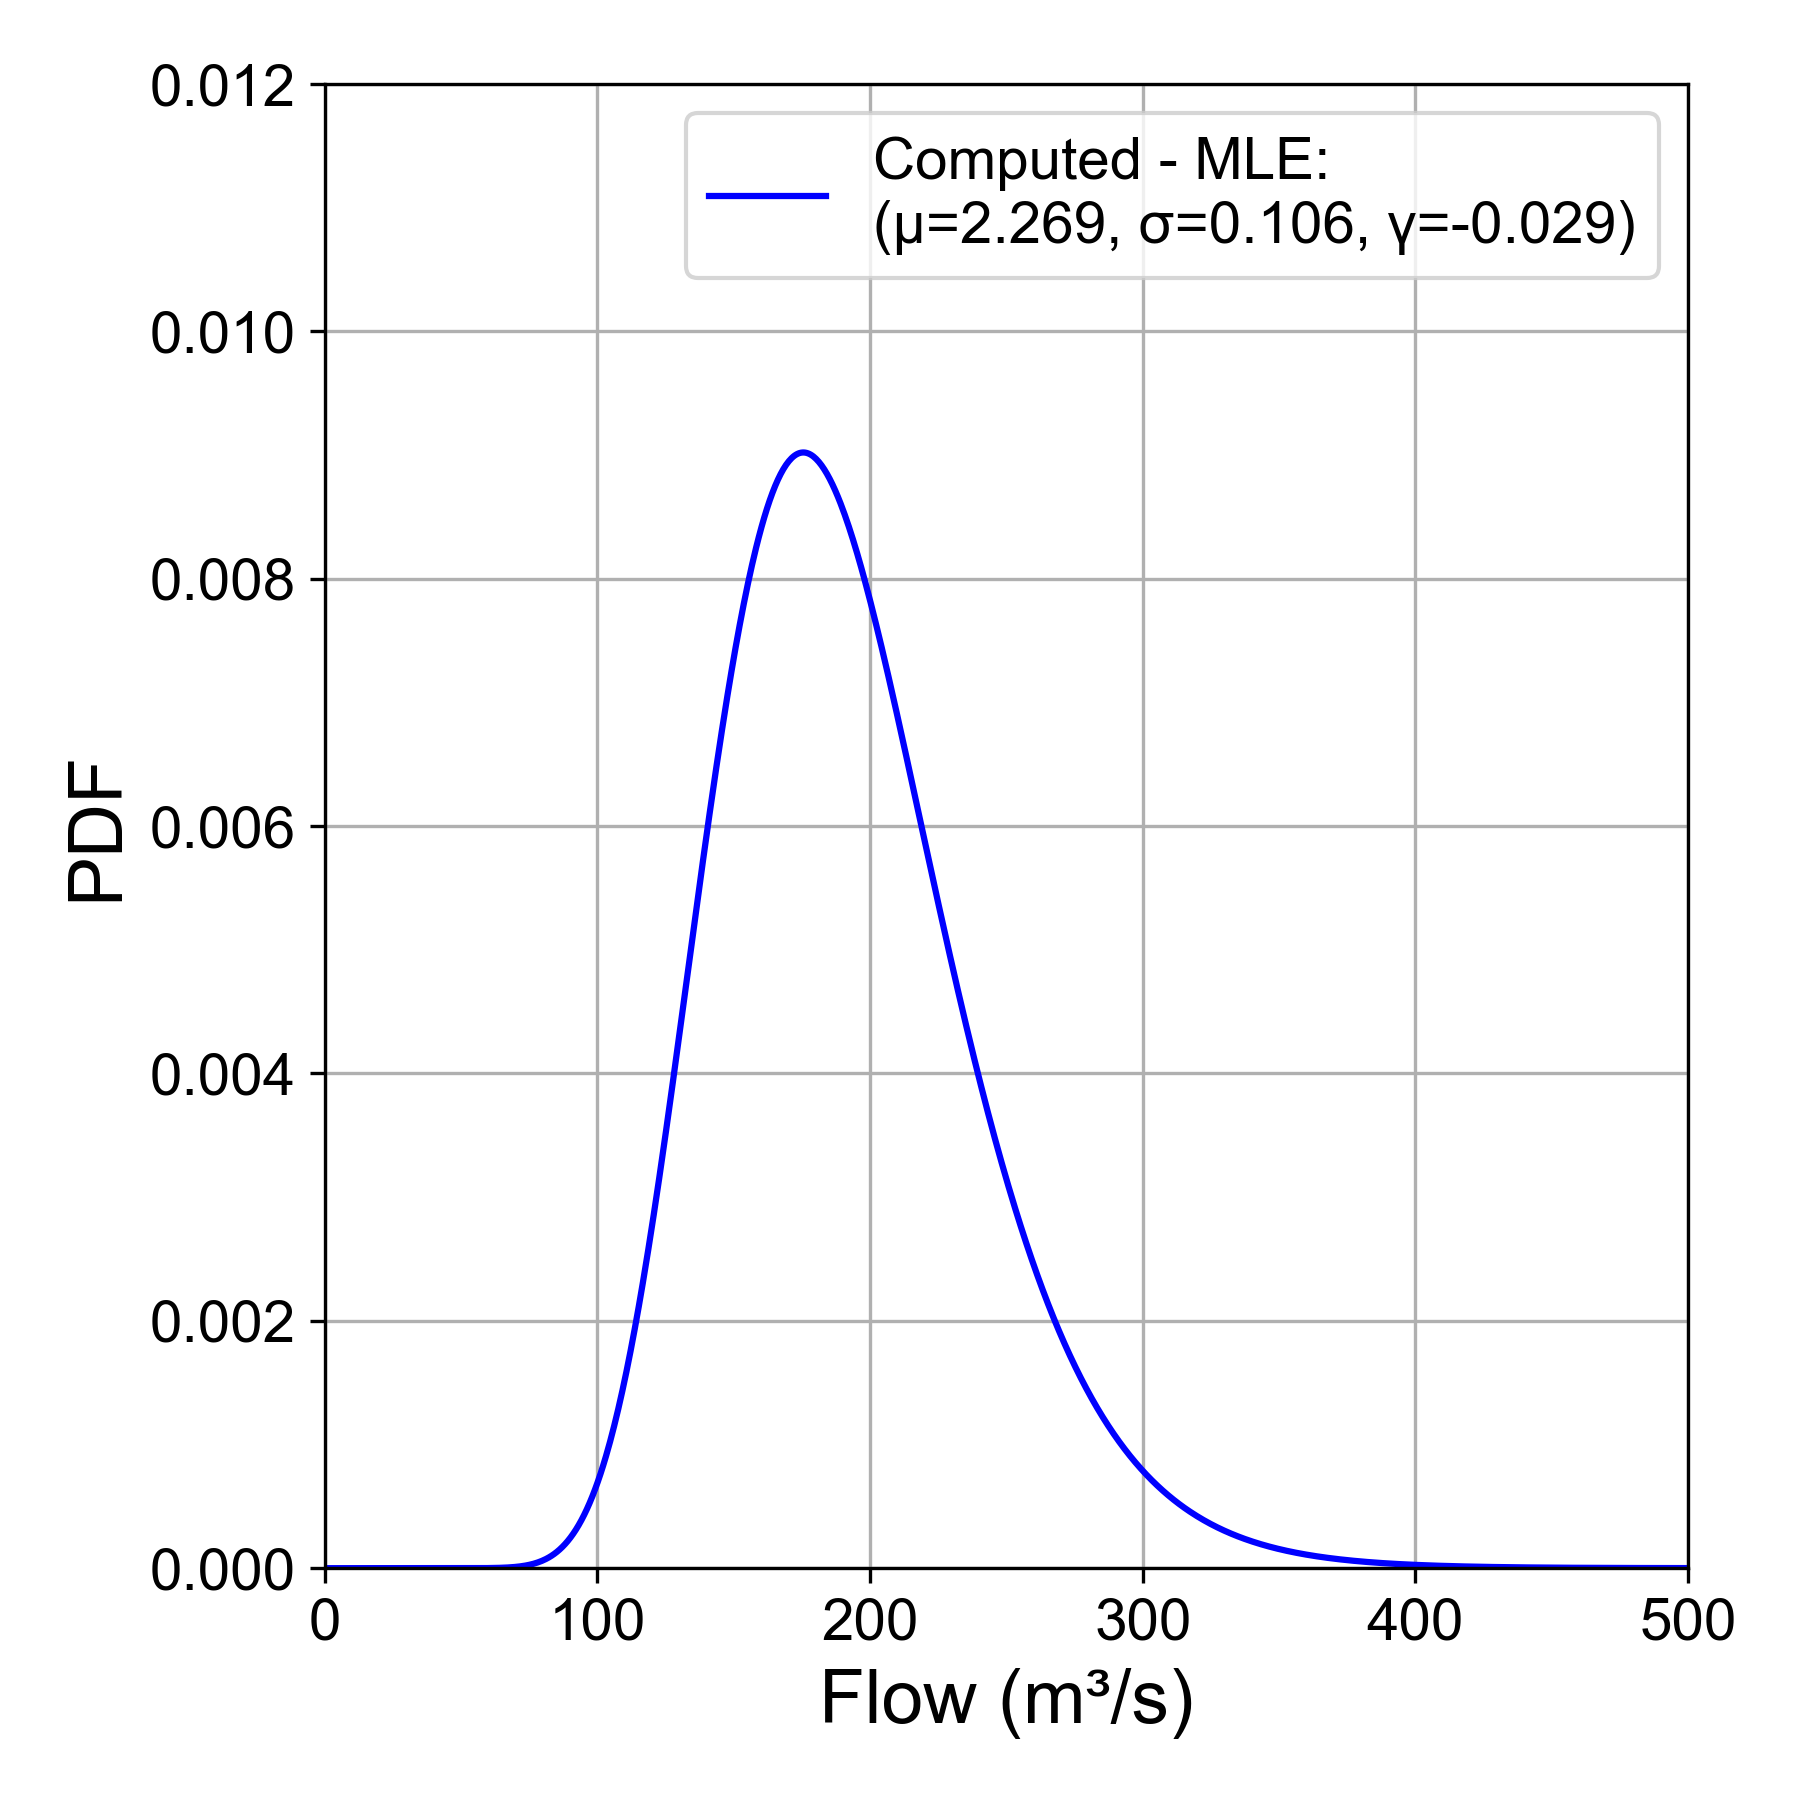
\includegraphics[width=1\linewidth]{_plots/HRA_LP3_MLE.png}
    \caption{LP3 distribution using the MLE method for the Harricana River dataset.}
    \label{fig:HRA_LP3_MLE}
\end{figure}

\begin{figure}[ht!]
    \centering
    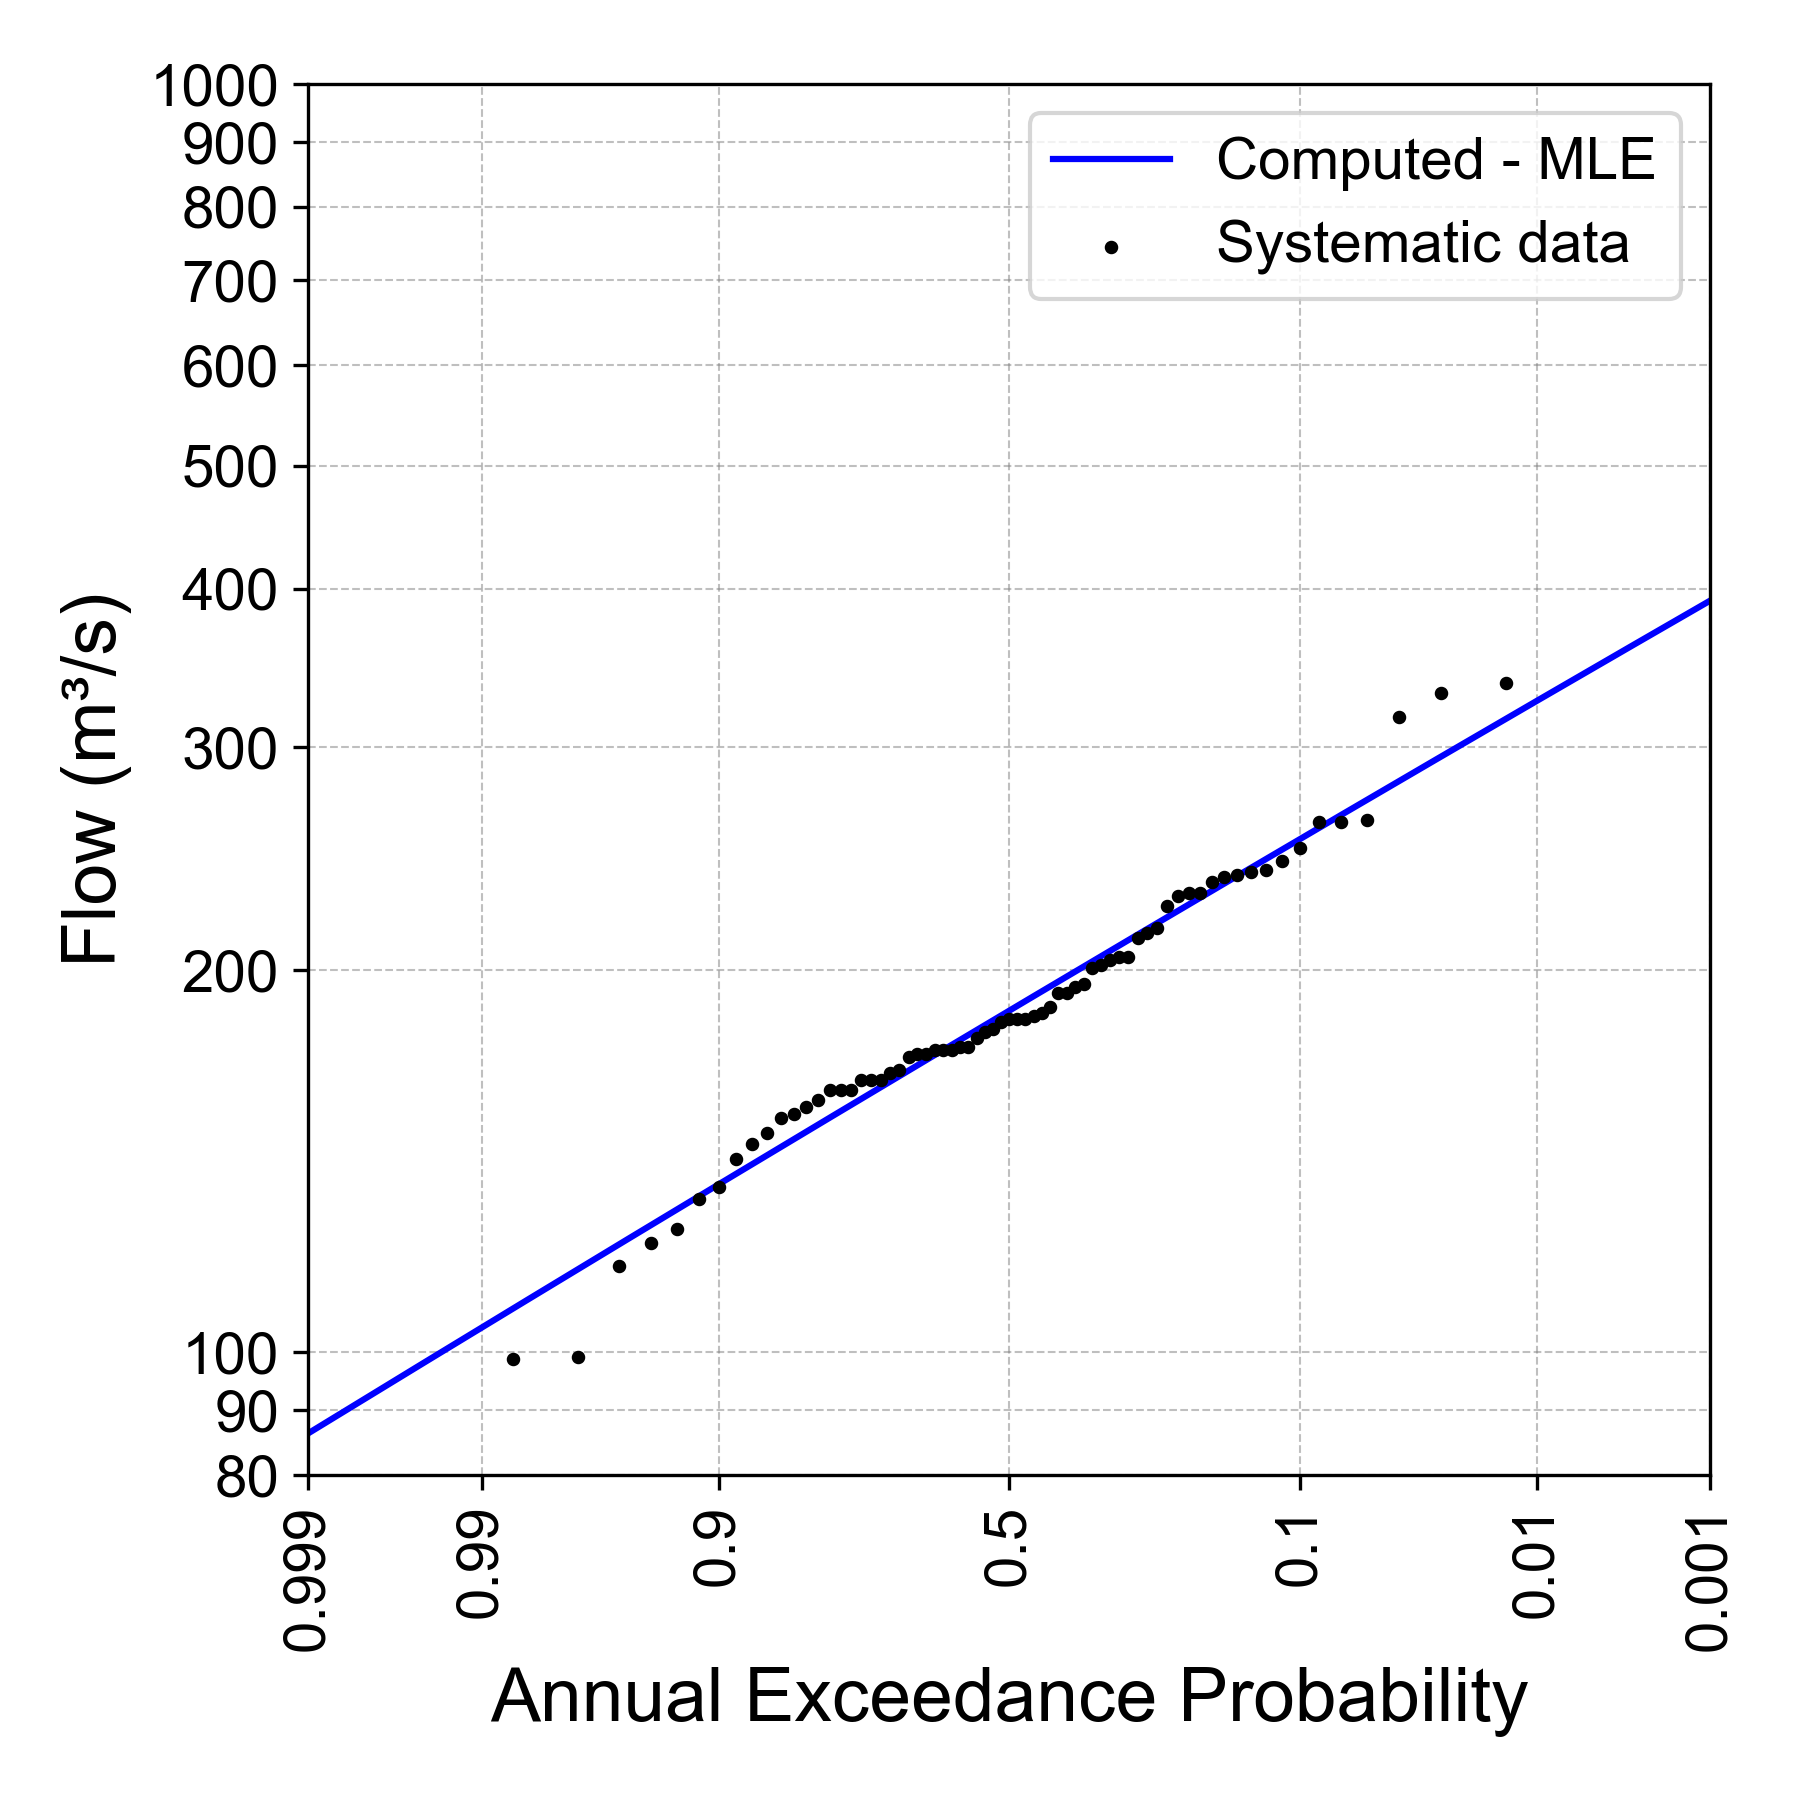
\includegraphics[width=1\linewidth]{_plots/HRA_flood_quantiles_MLE.png}
    \caption{Flood frequency curve using the MLE method for the Harricana River dataset.}
    \label{fig:HRA_flood_quantiles_MLE}
\end{figure}

The adaptive DE-MCzS algorithm demonstrates stable and efficient performance, with acceptance rates ranging from 0.525 to 0.533 across the five chains, as shown in Table \ref{table:HRA_acceptance}. Convergence diagnostics (Table \ref{table:HRA_Rhat}), indicate excellent chain convergence with $\hat{R}$ values near 1 for all parameters. The Effective Sample Size (ESS) is sufficiently high for $\mu$ and $\sigma$, although a lower ESS $\gamma$ suggests potential inefficiencies in sampling. Posterior marginal distributions and trace plots of $\mu, \sigma$ and $\gamma$ (Figure \ref{fig:HRA_posterior_combined_lp3}) further demonstrate stationary, well-mixed chains, and well-constrained parameter estimates, indicating an effective exploration of the posterior space.

\begin{figure*}[ht!]
    \centering
    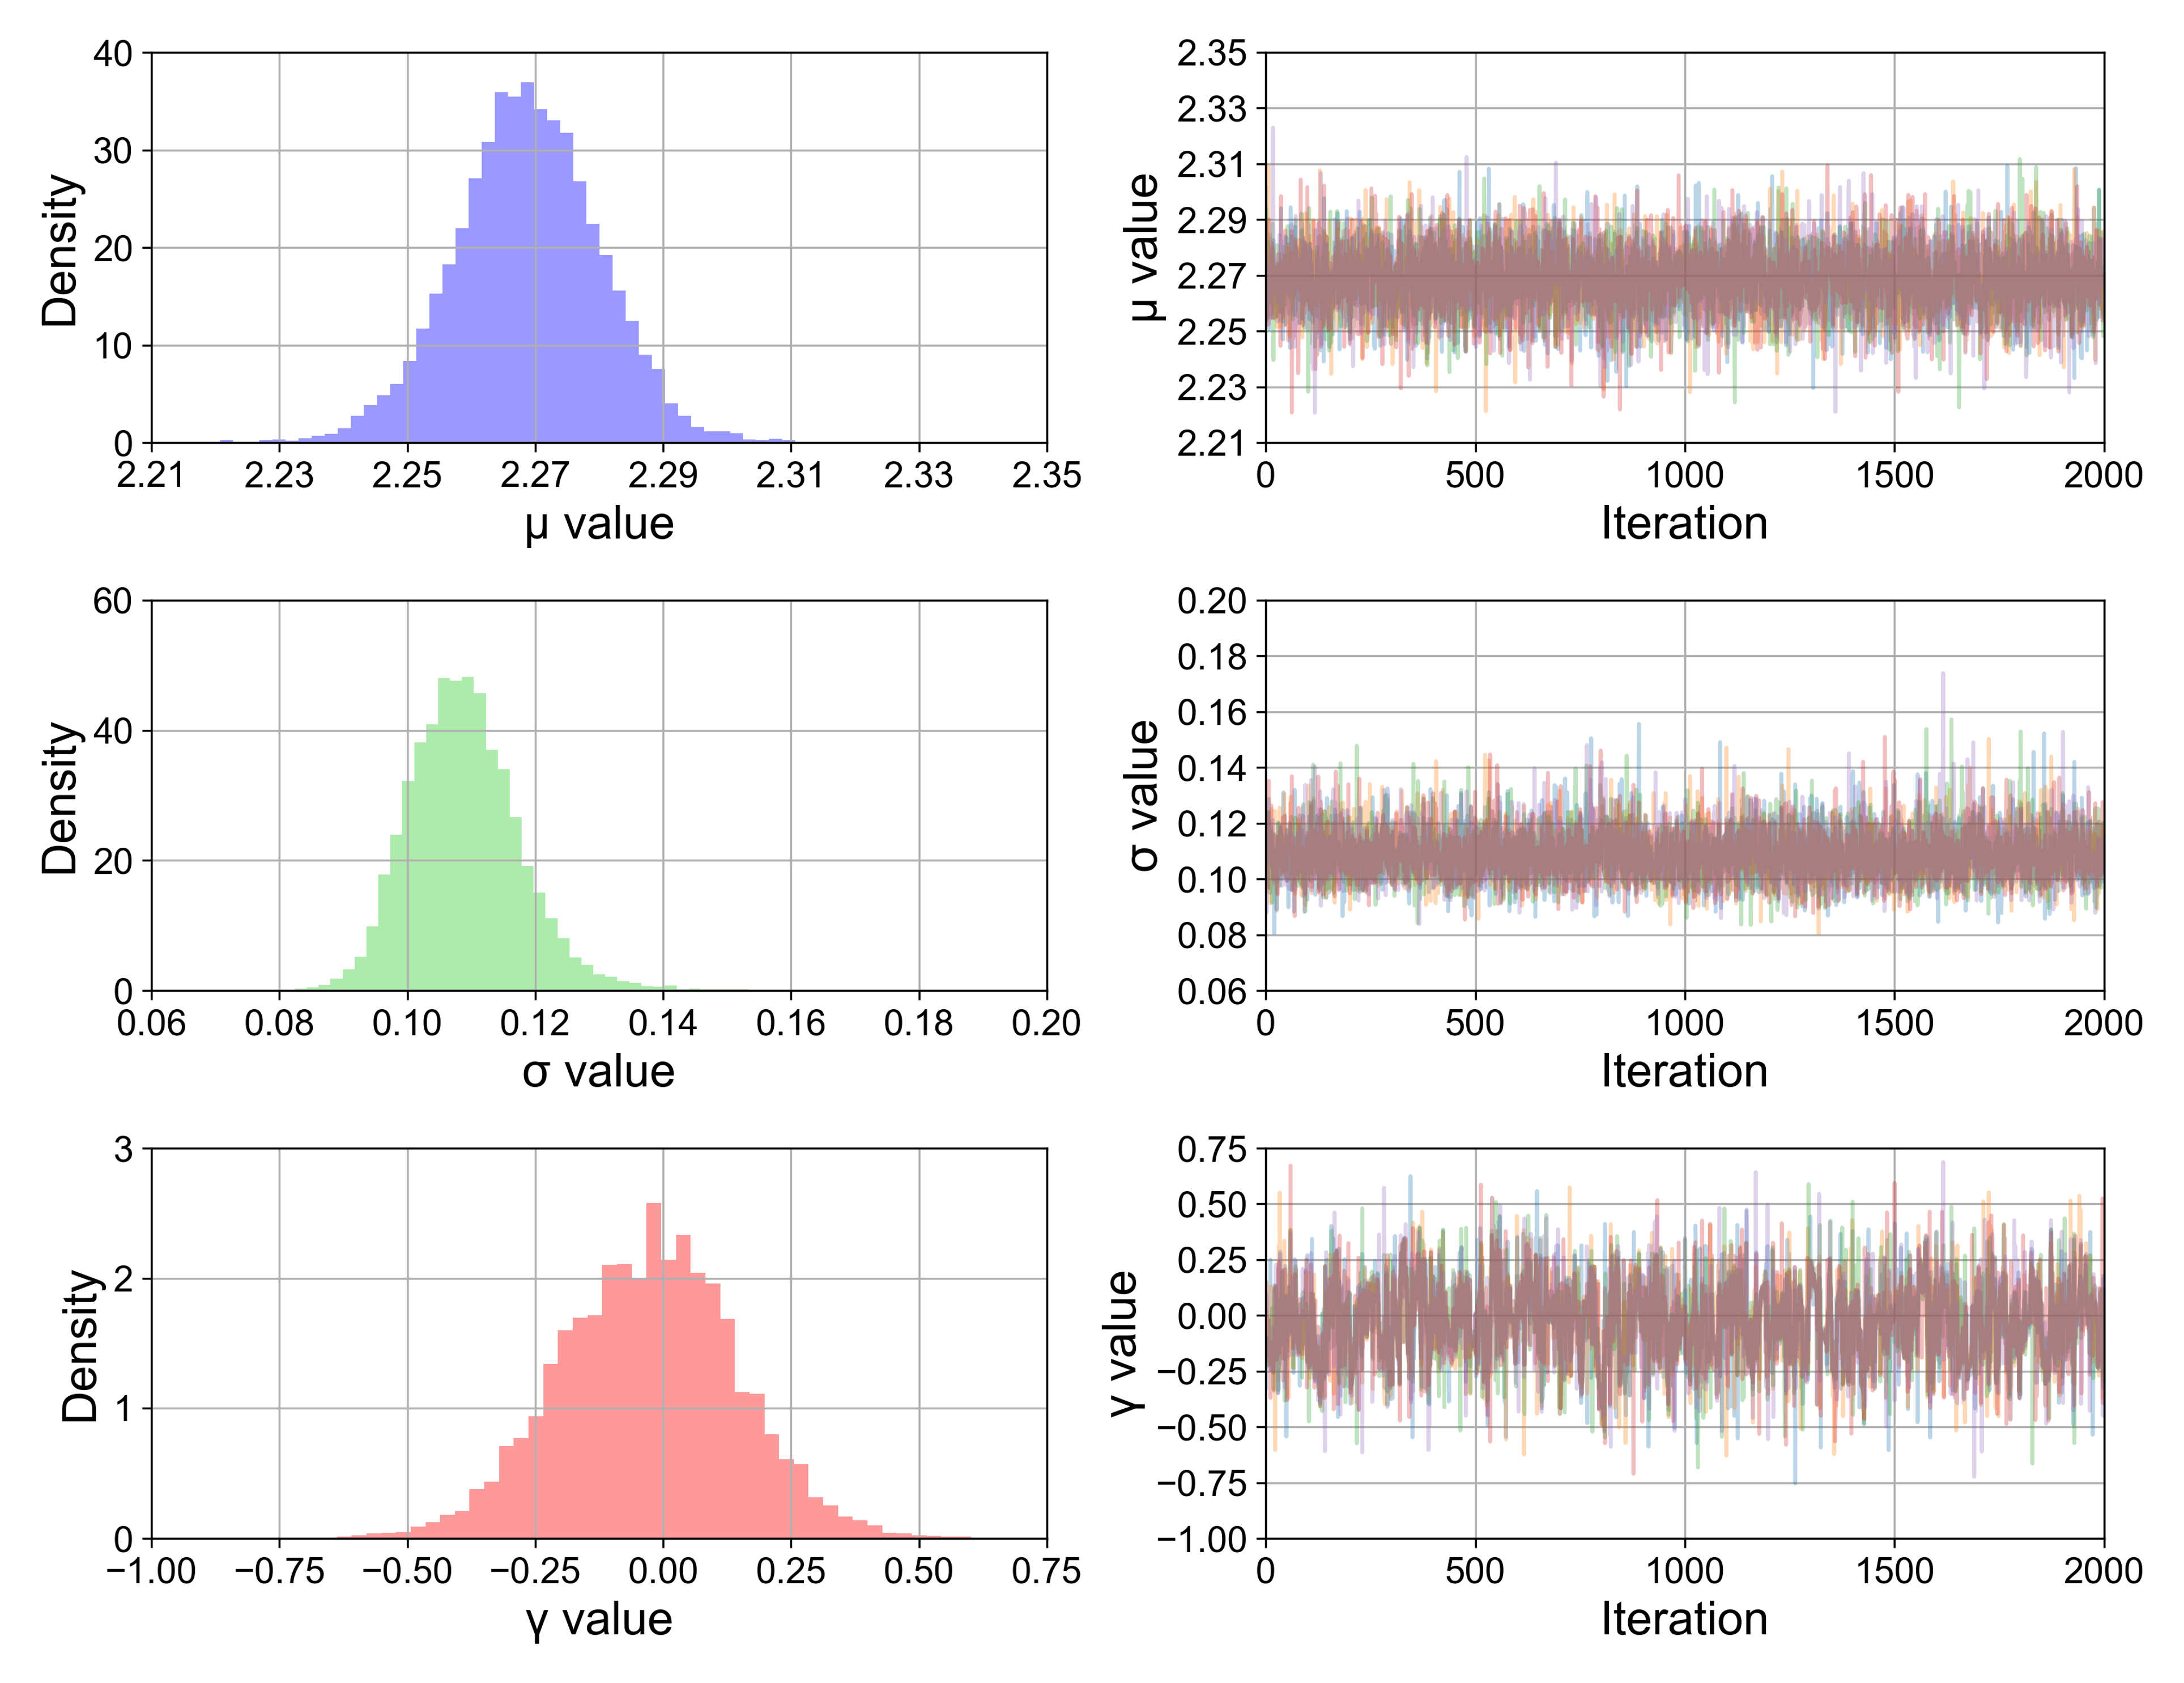
\includegraphics[width=1\linewidth]{_plots/HRA_posterior_combined_lp3.png}
    \caption{Posterior marginal distributions and trace plots for the $\mu$, $\sigma$, and $\gamma$ of LP3 distribution, derived from the Bayesian analysis of the Harricana River dataset. The trace plots checks convergence and efficient posterior sampling using the DE-MCzS algorithm.}
    \label{fig:HRA_posterior_combined_lp3}
\end{figure*}

\renewcommand{\arraystretch}{1.2}
% \begin{table}[H]
% \centering
% \caption{Acceptance rates for the DE-MCzS algorithm applied to the Harricana River dataset.}
% \begin{tabular}{l c c}
% \hline
% Chain No. & Number of Iterations & Acceptance Rate\\ \hline
% 1 & 2000 & 0.532 \\
% 2 & 2000 & 0.525 \\
% 3 & 2000 & 0.530 \\
% 4 & 2000 & 0.533 \\
% 5 & 2000 & 0.530 \\
% \hline
% \end{tabular}
% \label{table:HRA_acceptance}
% \end{table}

\renewcommand{\arraystretch}{1.2}
\begin{table}[H]
\centering
\caption{Acceptance rates for the DE-MCzS algorithm applied to the Harricana River dataset.}
\begin{tabular}{l c c c c c}
\hline
Chain No. &  1 & 2 & 3 & 4 & 5\\ \hline
Acceptance Rate & 0.532 & 0525 & 0.530 & 0.533 & 0.530\\
Iterations & 2000 & 2000 & 2000 & 2000 &2000 \\
\hline
\end{tabular}
\label{table:HRA_acceptance}
\end{table}

\renewcommand{\arraystretch}{1.2}
\begin{table}[H]
\centering
\caption{Comparison of convergence diagnostics between Computed and BestFit results for the LP3 parameters estimated using the Harricana River dataset.}
\begin{tabular}{l c c c c}
\hline
 & \multicolumn{2}{c}{$\hat{R}$} & \multicolumn{2}{c}{ESS} \\ 
Parameter & Computed & BestFit & Computed & BestFit \\ \hline
$\mu$ & 0.9998 & 1.000 & 8,571 & 10,000 \\
$\sigma$ & 1.0000 & 1.000 & 8,950 & 9,372 \\
$\gamma$ & 1.0001 & 1.000 & 2,204 & 10,000 \\
\hline
\end{tabular}
\label{table:HRA_Rhat}
\end{table}

\begin{figure}[H]
    \centering
    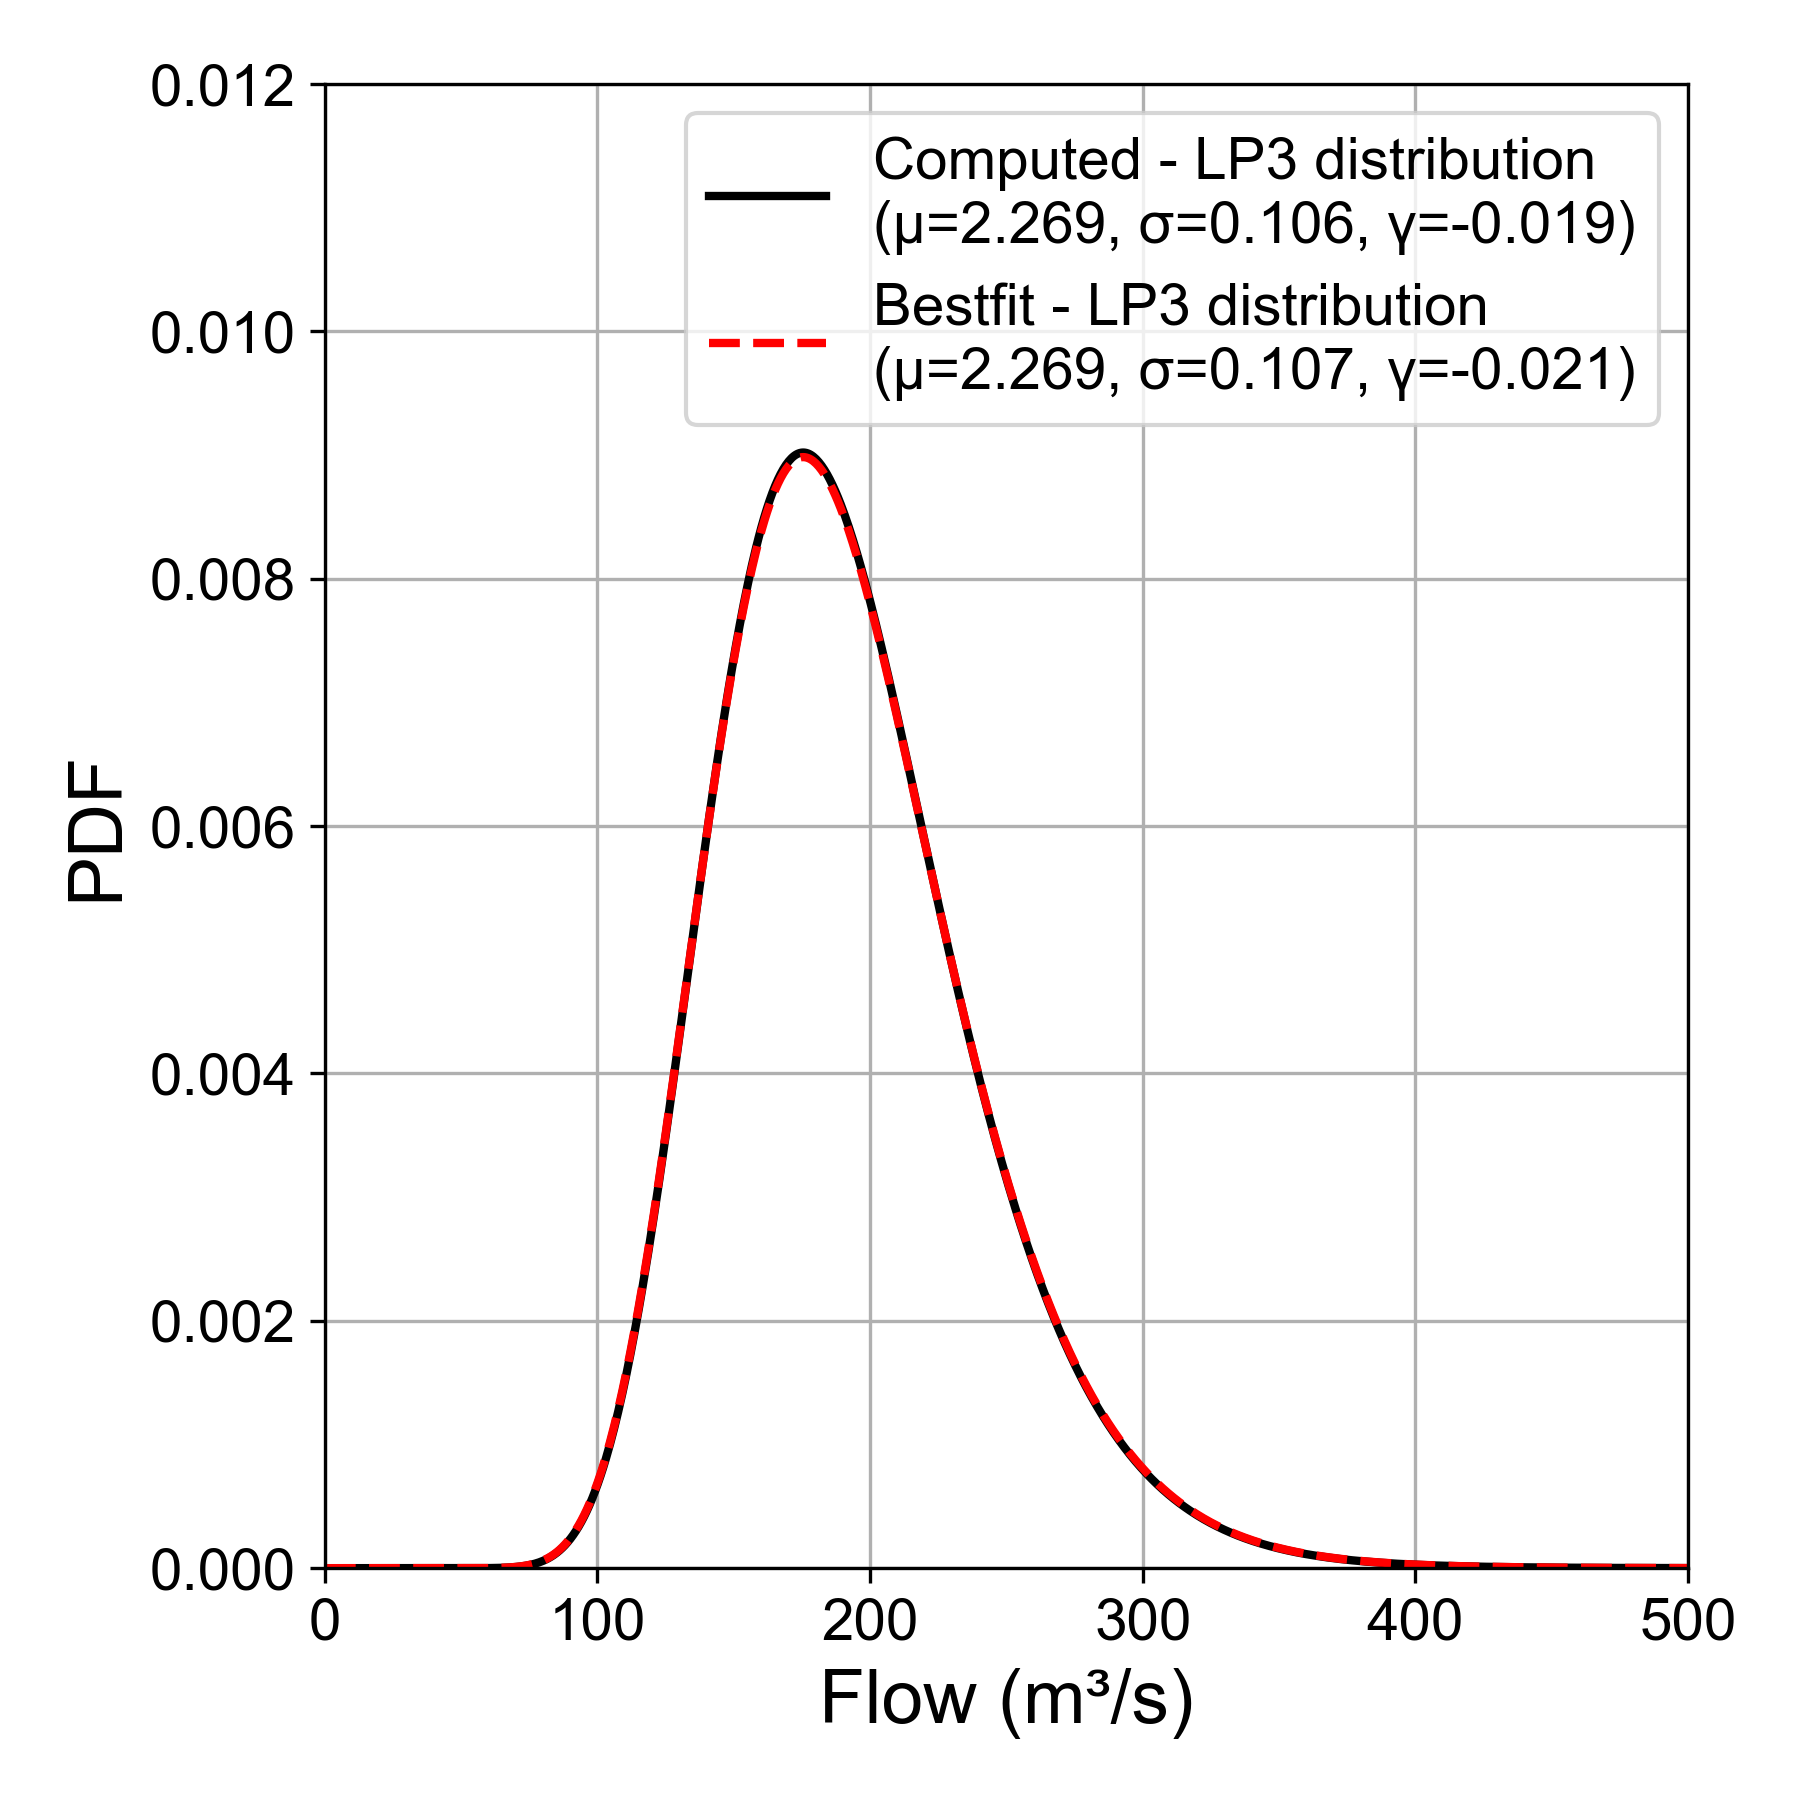
\includegraphics[width=1\linewidth]{_plots/HRA_LP3_comparison.png}
    \caption{Comparison of the posterior mode LP3 distribution with the BestFit results for the Harricana River dataset. }
    \label{fig:HRA_LP3_comparison}
\end{figure}

In verification, the computed LP3 distribution at the posterior mode (Figure \ref{fig:HRA_LP3_comparison}) aligns exceptionally well with the results obtained from BestFit results. With the same noise term applied (labeled as noise testing), we were able to reproduce the posterior predictive distributions and their 90\% credible intervals on the flood frequency curve (Figure \ref{fig:HRA_bayesian_flood_quantiles_lp3}). Overall, an excellent consistency was achieved with BestFit. Minor discrepancies at the distribution tails likely result from differences in the random seed generation.

\begin{figure*}[ht!]
    \centering
    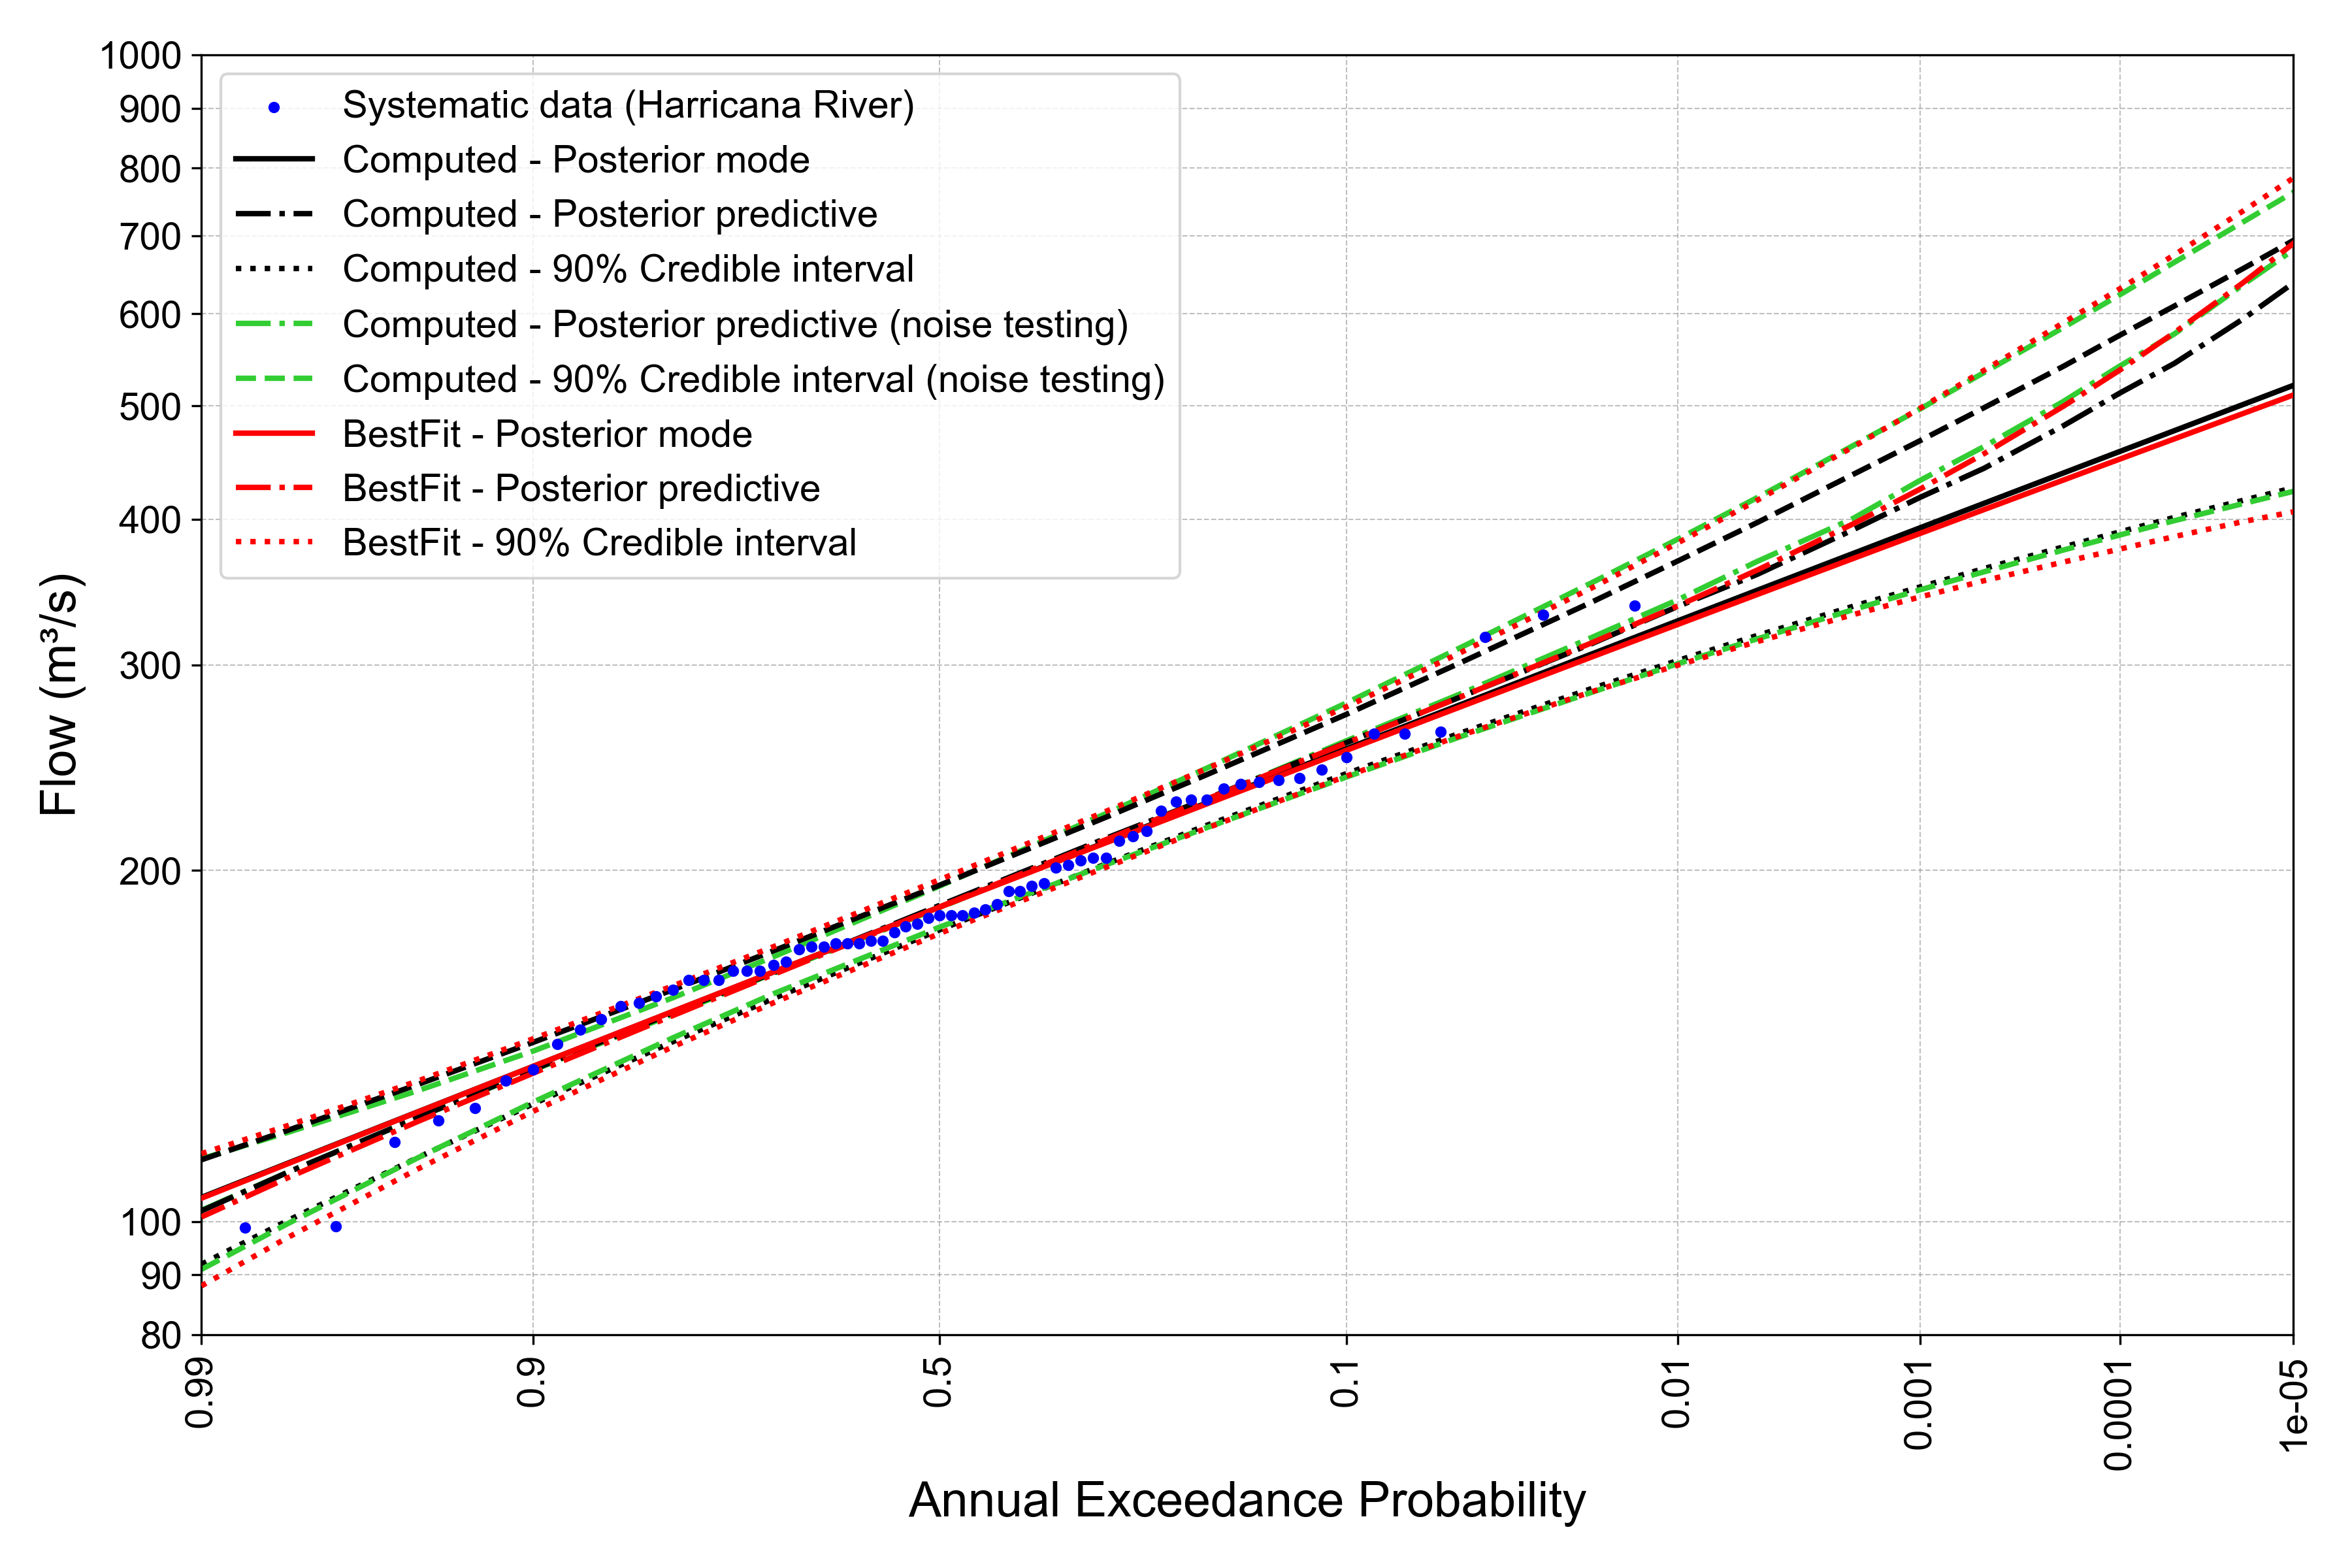
\includegraphics[width=1\linewidth]{_plots/HRA_bayesian_flood_quantiles_lp3.png}
    \caption{Comparison of Bayesian flood frequency curves with BestFit for the Harricana River dataset. Noise testing refers to the use of the same perturbation term as employed in BestFit to ensure consistency in model comparisons.}
    \label{fig:HRA_bayesian_flood_quantiles_lp3}
\end{figure*}

\subsection{Case study 2: O.C. Fisher Dam, USA}

The second case study examines both stationary FFA and NSFFA for the O.C. Fisher Dam dataset. The stationary FFA assumes constant parameters over time with uniform priors: 
\begin{align*}
    Y \mid \mu, \sigma, \gamma &\sim \text{LP3}(\mu, \sigma, \gamma)\\
    \mu &\sim \text{Uniform}(0,3)\\
    \sigma &\sim \text{Uniform}(0,2)\\
    \gamma &\sim \text{Uniform}(-2,2)
\end{align*}

The NSFFA models incorporate time-dependent trends for the location parameter ($\mu$), while $\sigma$ and $\gamma$ have the same prior as the stationary FFA model:
\begin{align*}
    Y \mid \mu_t, \sigma, \gamma &\sim \text{LP3}(\mu_t, \sigma, \gamma)\\
    \mu_t &=\beta_0 + \beta_1 \cdot t \quad \text{(linear)}\\
    \mu_t &=\beta_0 \cdot \exp(\beta_1 \cdot t ) \quad \text{ (exponential)}\\
    \beta_0 &\sim \text{Uniform}(0,3)\\
    \beta_1 &\sim \text{Uniform}(-1,1)
\end{align*}


\begin{figure}[H]
    \centering
    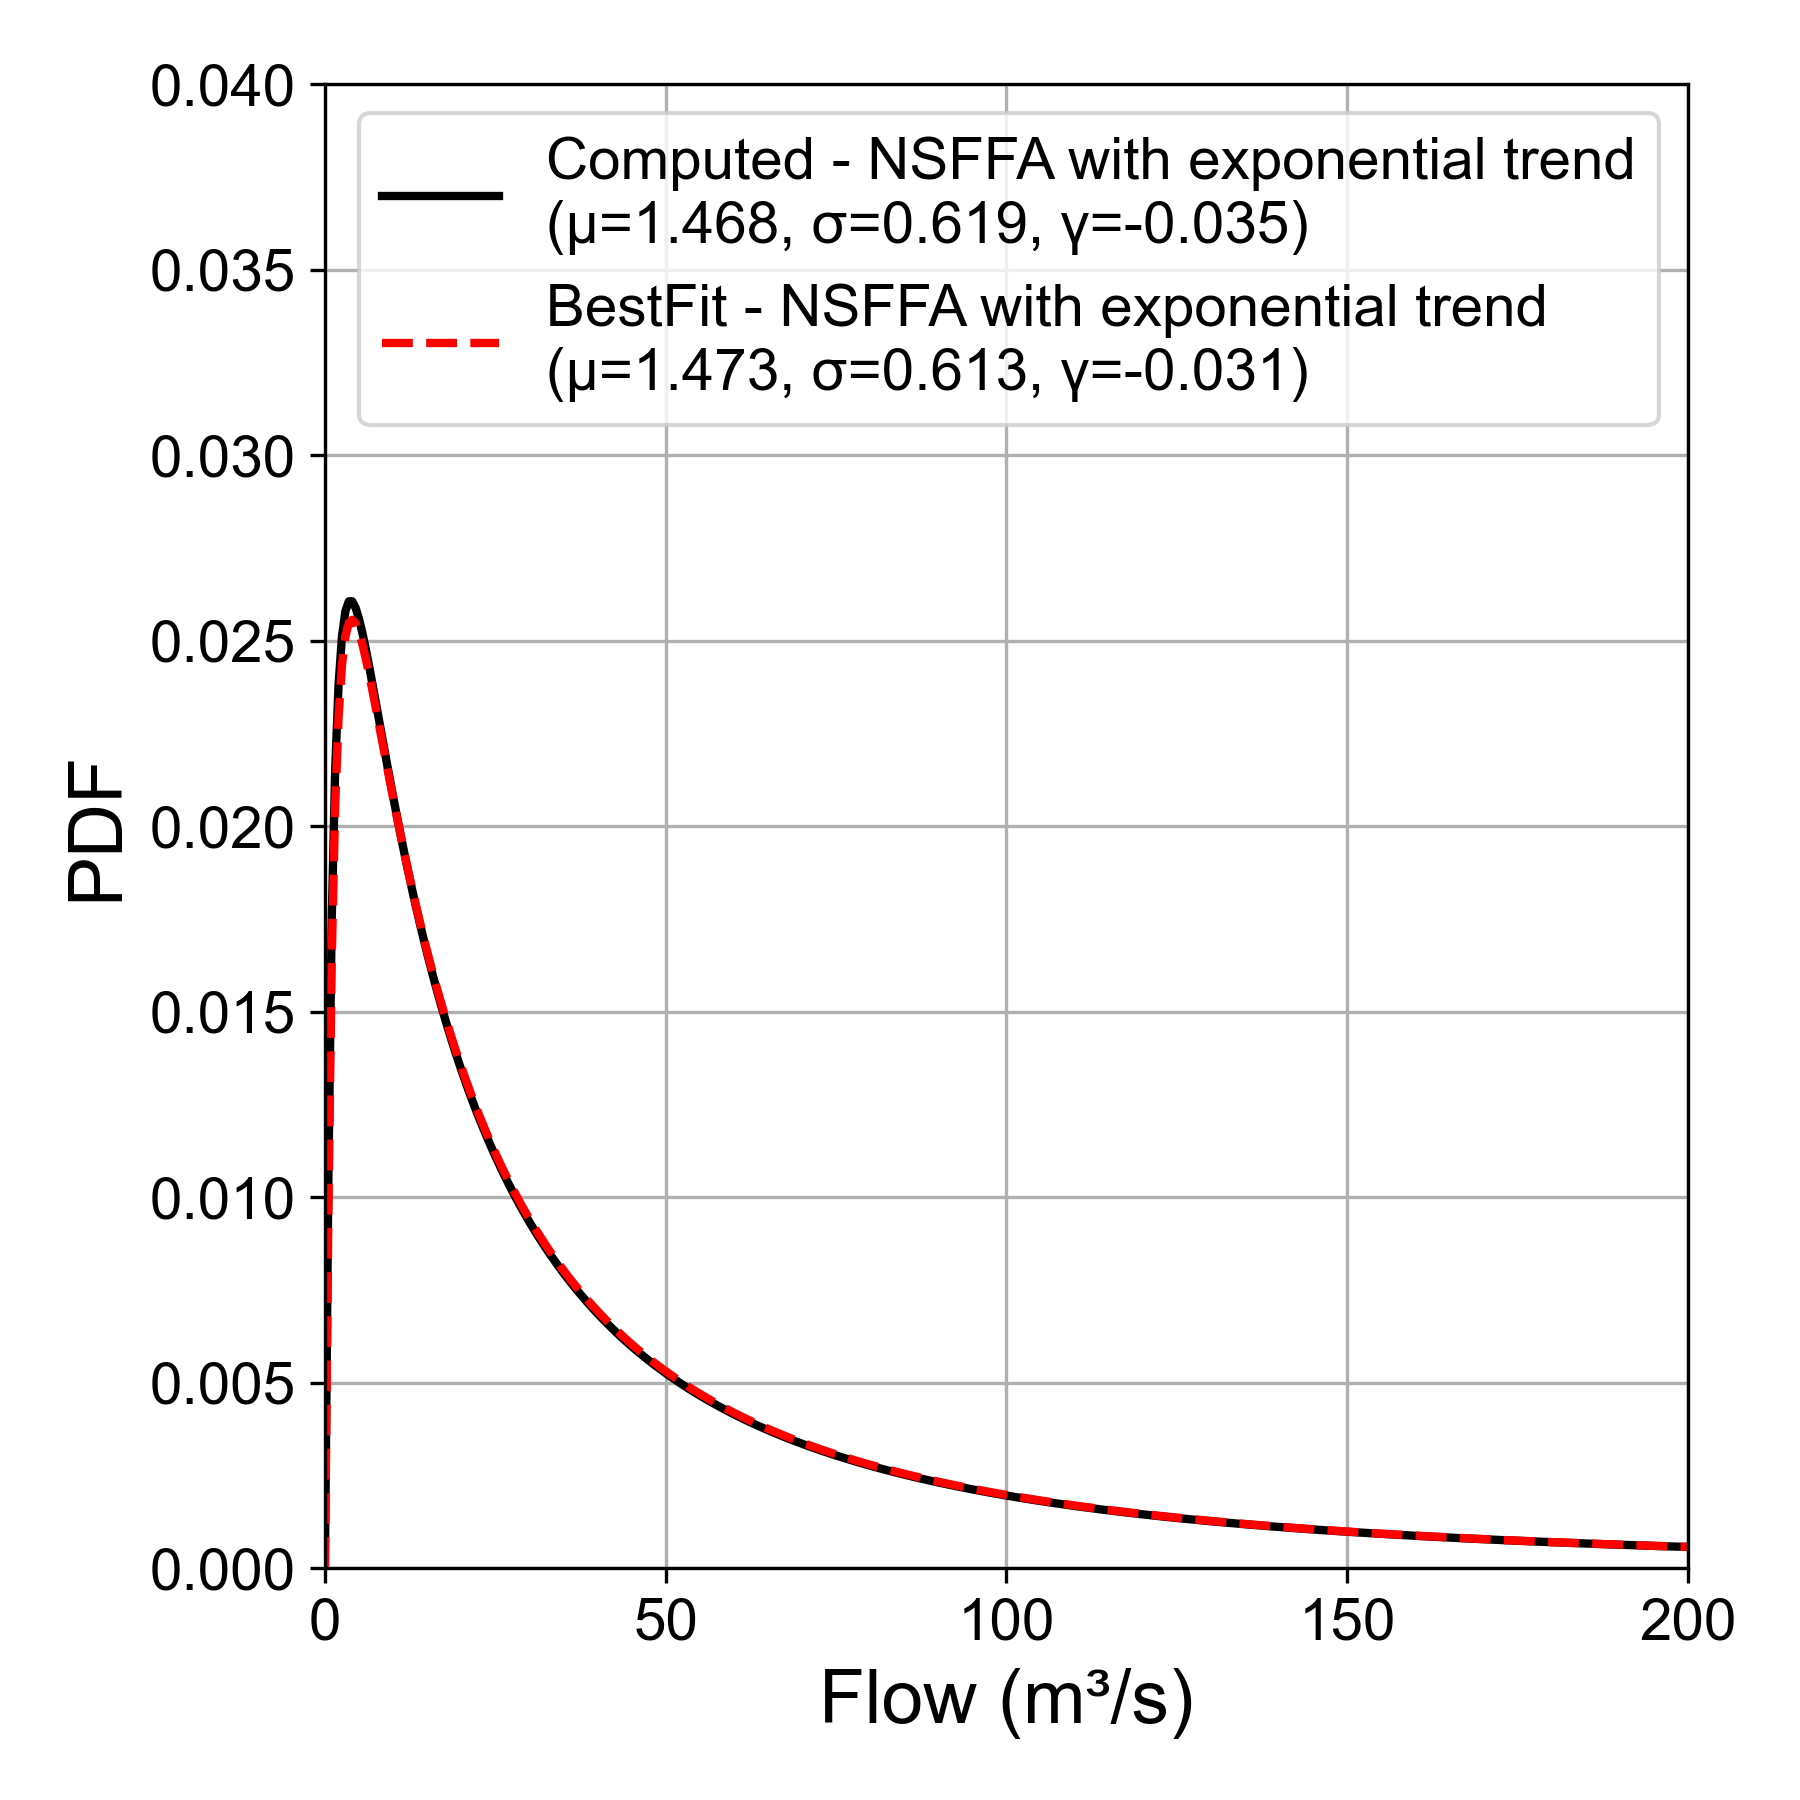
\includegraphics[width=1\linewidth]{_plots/OCD_LP3_exponential_mu_comparison.png}
    \caption{Comparison of the posterior mode LP3 distribution with the BestFit results under the linear trend NSFFA model for the Fisher Dam dataset.}
    \label{fig:OCD_LP3_exponential_mu_comparison}
\end{figure}

The posterior mode estimates for the three models — stationary FFA, NSFFA with a linear trend, and NSFFA with an exponential trend - were benchmarked against the results from BestFit (Table \ref{table:OCD_comparison_computed_bestfit}). Overall, the computed parameters demonstrate a strong agreement with BestFit results. The exponential trend model shows notable deviations in parameters $\beta_1$ and $\gamma$. However, the LP3 distribution derived from the this model (Figure \ref{fig:OCD_LP3_exponential_mu_comparison}) closely aligns with BestFit. Performance evaluation of the adaptive DE-MCzS algorithm and verification of flood frequency curves are presented in Appendix C. The discrepancies observed in the posterior predictive distributions and credible intervals can be attributed to variations in the noise term as shown in Figure \ref{fig:HRA_bayesian_flood_quantiles_lp3}.

\renewcommand{\arraystretch}{1.2}
\begin{table*}
\centering
\caption{Comparison of computed and BestFit posterior mode estimates for different models, including FFA, NSFFA (TI of 1949) with linear and exponential trends, using the Fisher Dam dataset.}
\begin{tabular}{llccc}
\hline
Model & Parameter & Computed & BestFit & \textbf{\% Difference} \\ \hline
Stationary FFA & $\mu$ & 1.303 & 1.300 & 0.17\% \\
& $\sigma$ & 0.699 & 0.696 & 0.50\% \\
& $\gamma$ & 0.178 & 0.178 & 0.11\% \\ \hline
NSFFA with linear trend & $\beta_0$ & 1.869 & 1.871 & -0.15\% \\
& $\beta_1$ & -0.0108 & -0.0109 & -1.12\% \\
& $\sigma$ & 0.614 & 0.613 & 0.21\% \\
& $\gamma$ & -0.048 & -0.047 & 1.44\% \\ \hline
NSFFA with exponential trend & $\beta_0$ & 1.934 & 1.871 & 3.37\% \\
& $\beta_1$ & -0.00811 & -0.01091 & -25.62\% \\
& $\sigma$ & 0.619 & 0.613 & 1.01\% \\
& $\gamma$ & -0.0345 & -0.0469 & -26.49\% \\ \hline
\end{tabular}
\label{table:OCD_comparison_computed_bestfit}
\end{table*}

\begin{figure}[H]
    \centering
    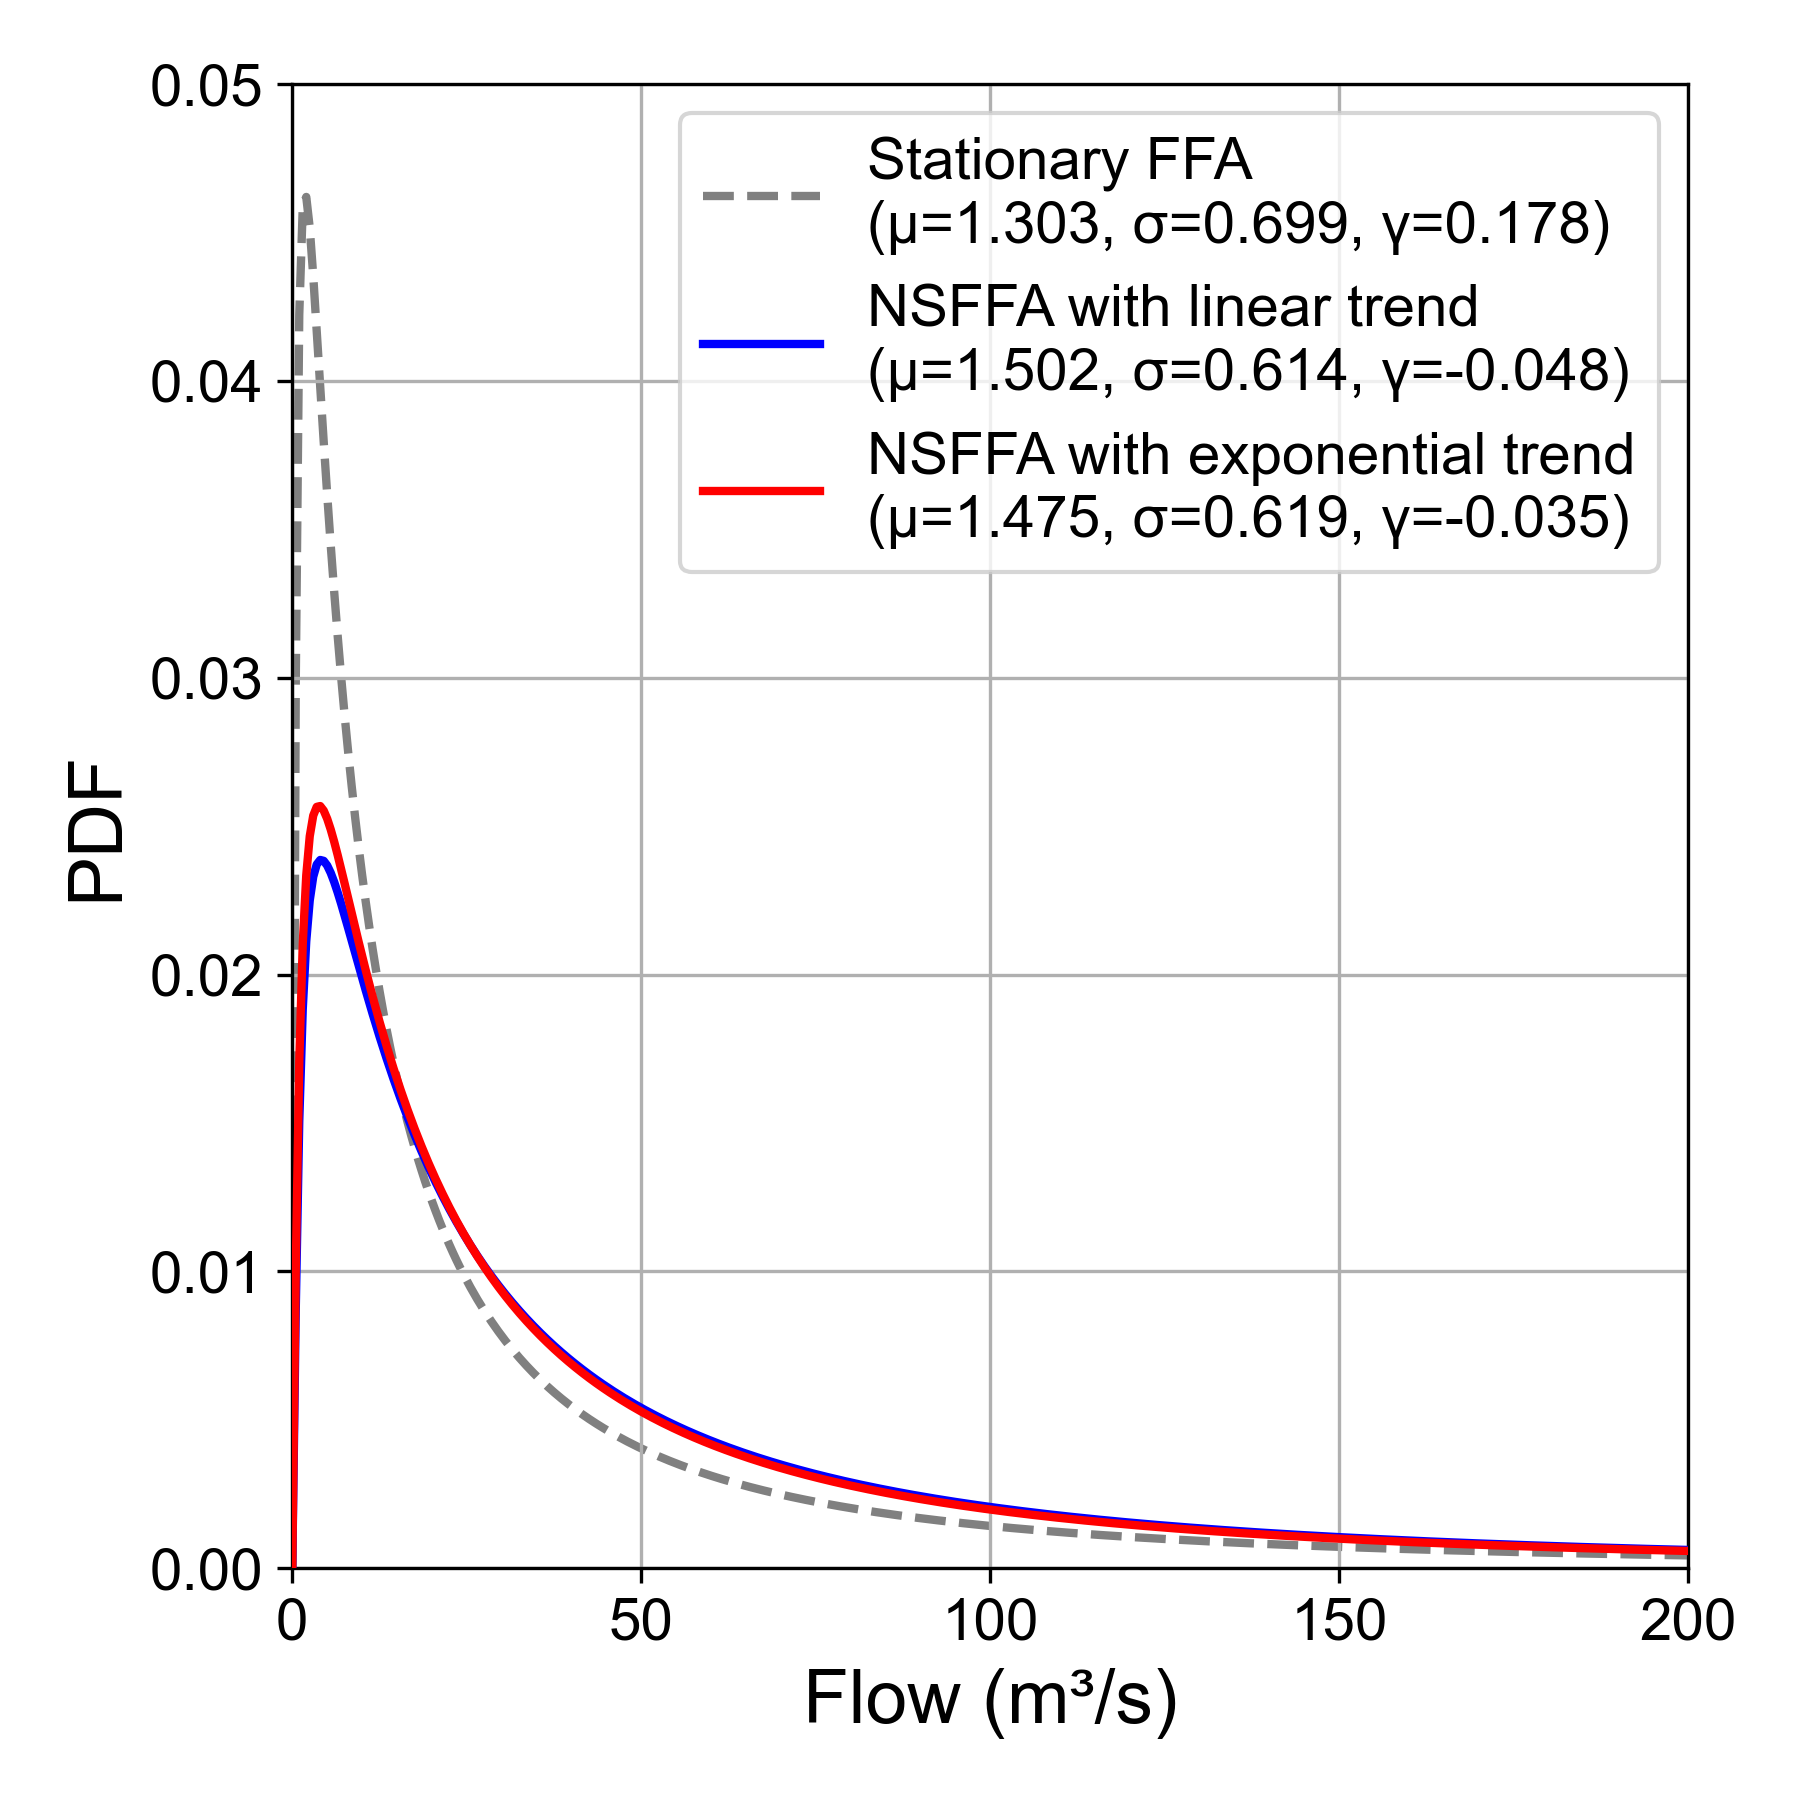
\includegraphics[width=1\linewidth]{_plots/OCD_LP3_nonstationary_comparison.png}
    \caption{Comparison of posterior mode LP3 distribution for FFA and NSFFA using the Fisher Dam dataset, with the middle year (1949) selected as the time index for analysis.}
    \label{fig:OCD_LP3_nonstationary_comparison}
\end{figure}

The LP3 distributions, shown in Figure \ref{fig:OCD_LP3_nonstationary_comparison}, were analyzed with the middle year (1949) selected as the time index for NSFFA. The stationary FFA model exhibits a higher peak density, reflecting concentrated probabilities near the central tendency, while the NSFFA models (both linear and exponential trends) show reduced peak densities and heavier tails, indicating greater uncertainty. These differences are further reflected in flood frequency curves (Figure \ref{fig:OCD_bayesian_flood_quantiles_lp3_linear_mu_TI}). The stationary FFA model aligns closely with observed data, particularly for frequent AEPs. In contrast, the NSFFA curves are generally flatter, predicting higher flows for frequent events but significantly lower flows for extreme events. Between the linear and exponential trend NSFFA models, the resulting distributions are broadly similar, with minor differences in peak density. This suggests that the choice of trend type has a negligible effect on the flood frequency curves for the Fisher Dam dataset.

Figure \ref{fig:OCD_LP3_linear_mu_comparison_TI} explores the impact of time index selection on LP3 distributions under the linear trend model. Earlier time indices, such as 1919 ($\mu = 1.825$), correspond to higher mean flow values and exhibit lower peak densities and higher variance. As the time index advances toward future years (e.g., 2049, $\mu = 0.423$), the distribution become narrower with higher peak densities and lower variance. This indicates a systematic reduction in mean flows and increased concentration of probabilities around smaller values. The impact of time index selection on flood frequency curves is illustrated in Figure \ref{fig:OCD_bayesian_flood_quantiles_lp3_linear_mu_TI} under the same model. Earlier TIs (e.g., 1919) predict higher flow values, while later TIs (e.g., 2049) yield lower flow values, which aligns with the observed decline in mean flow over time.

\begin{figure}[H]
    \centering
    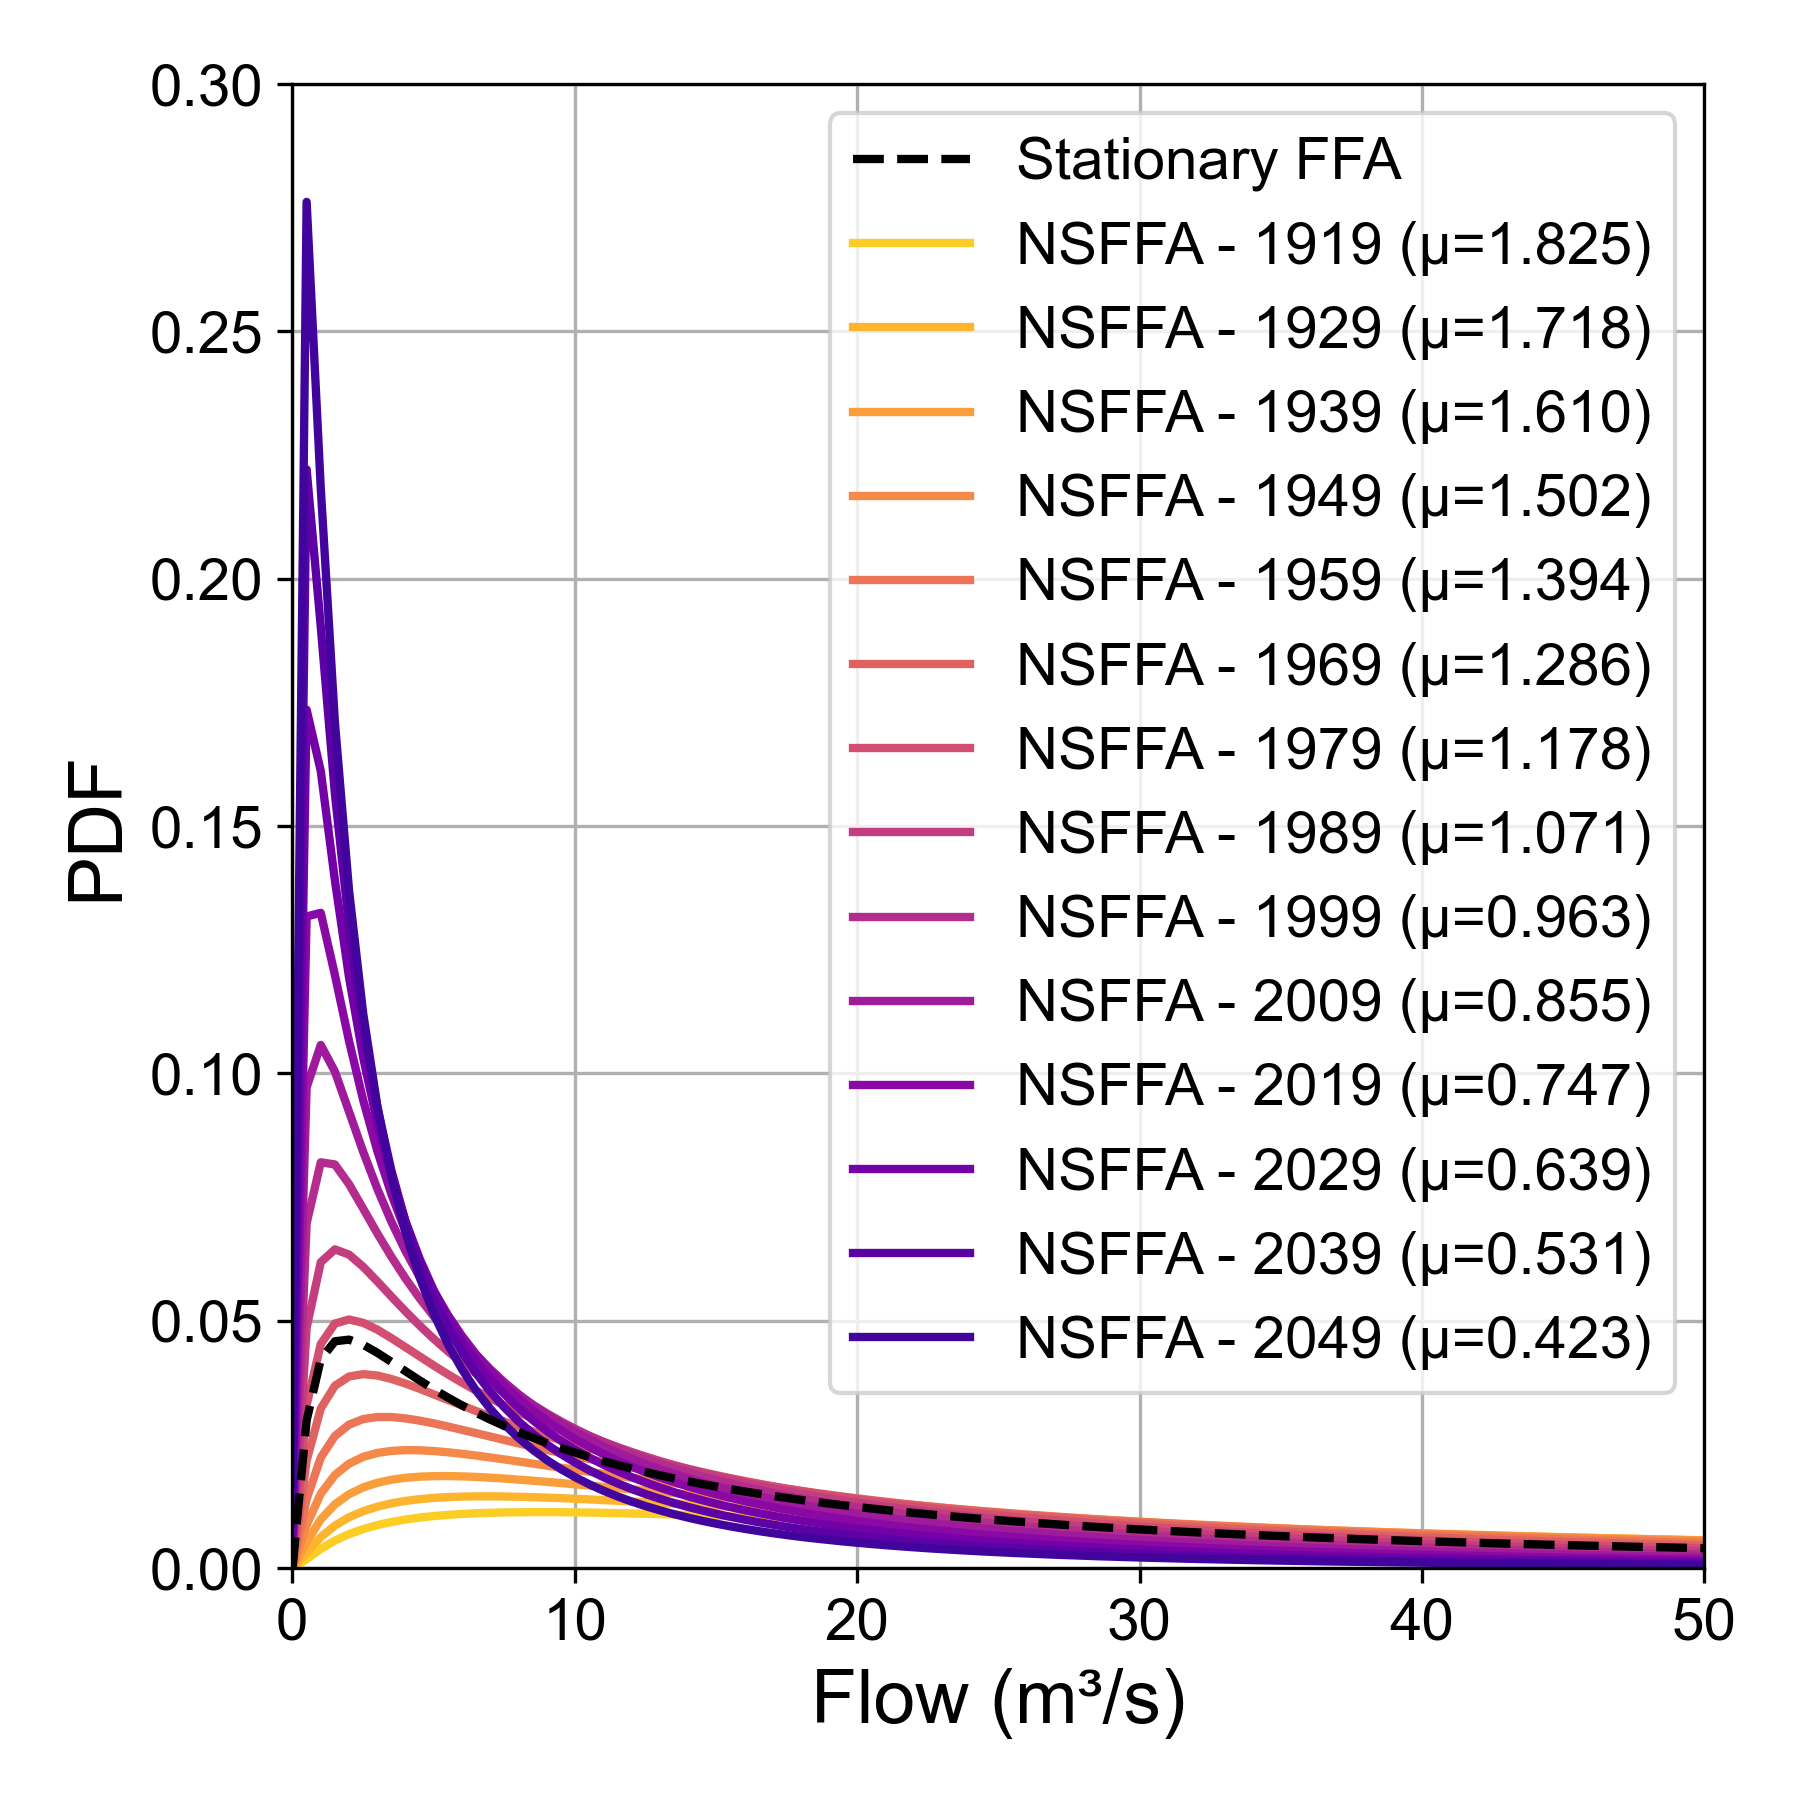
\includegraphics[width=1\linewidth]{_plots/OCD_LP3_linear_mu_comparison_TI.png}
    \caption{Impact of time index selection on posterior mode LP3 distributions under the linear trend NSFFA model for the Fisher Dam dataset.}
    \label{fig:OCD_LP3_linear_mu_comparison_TI}
\end{figure}

\begin{figure*}[ht!]
    \centering
    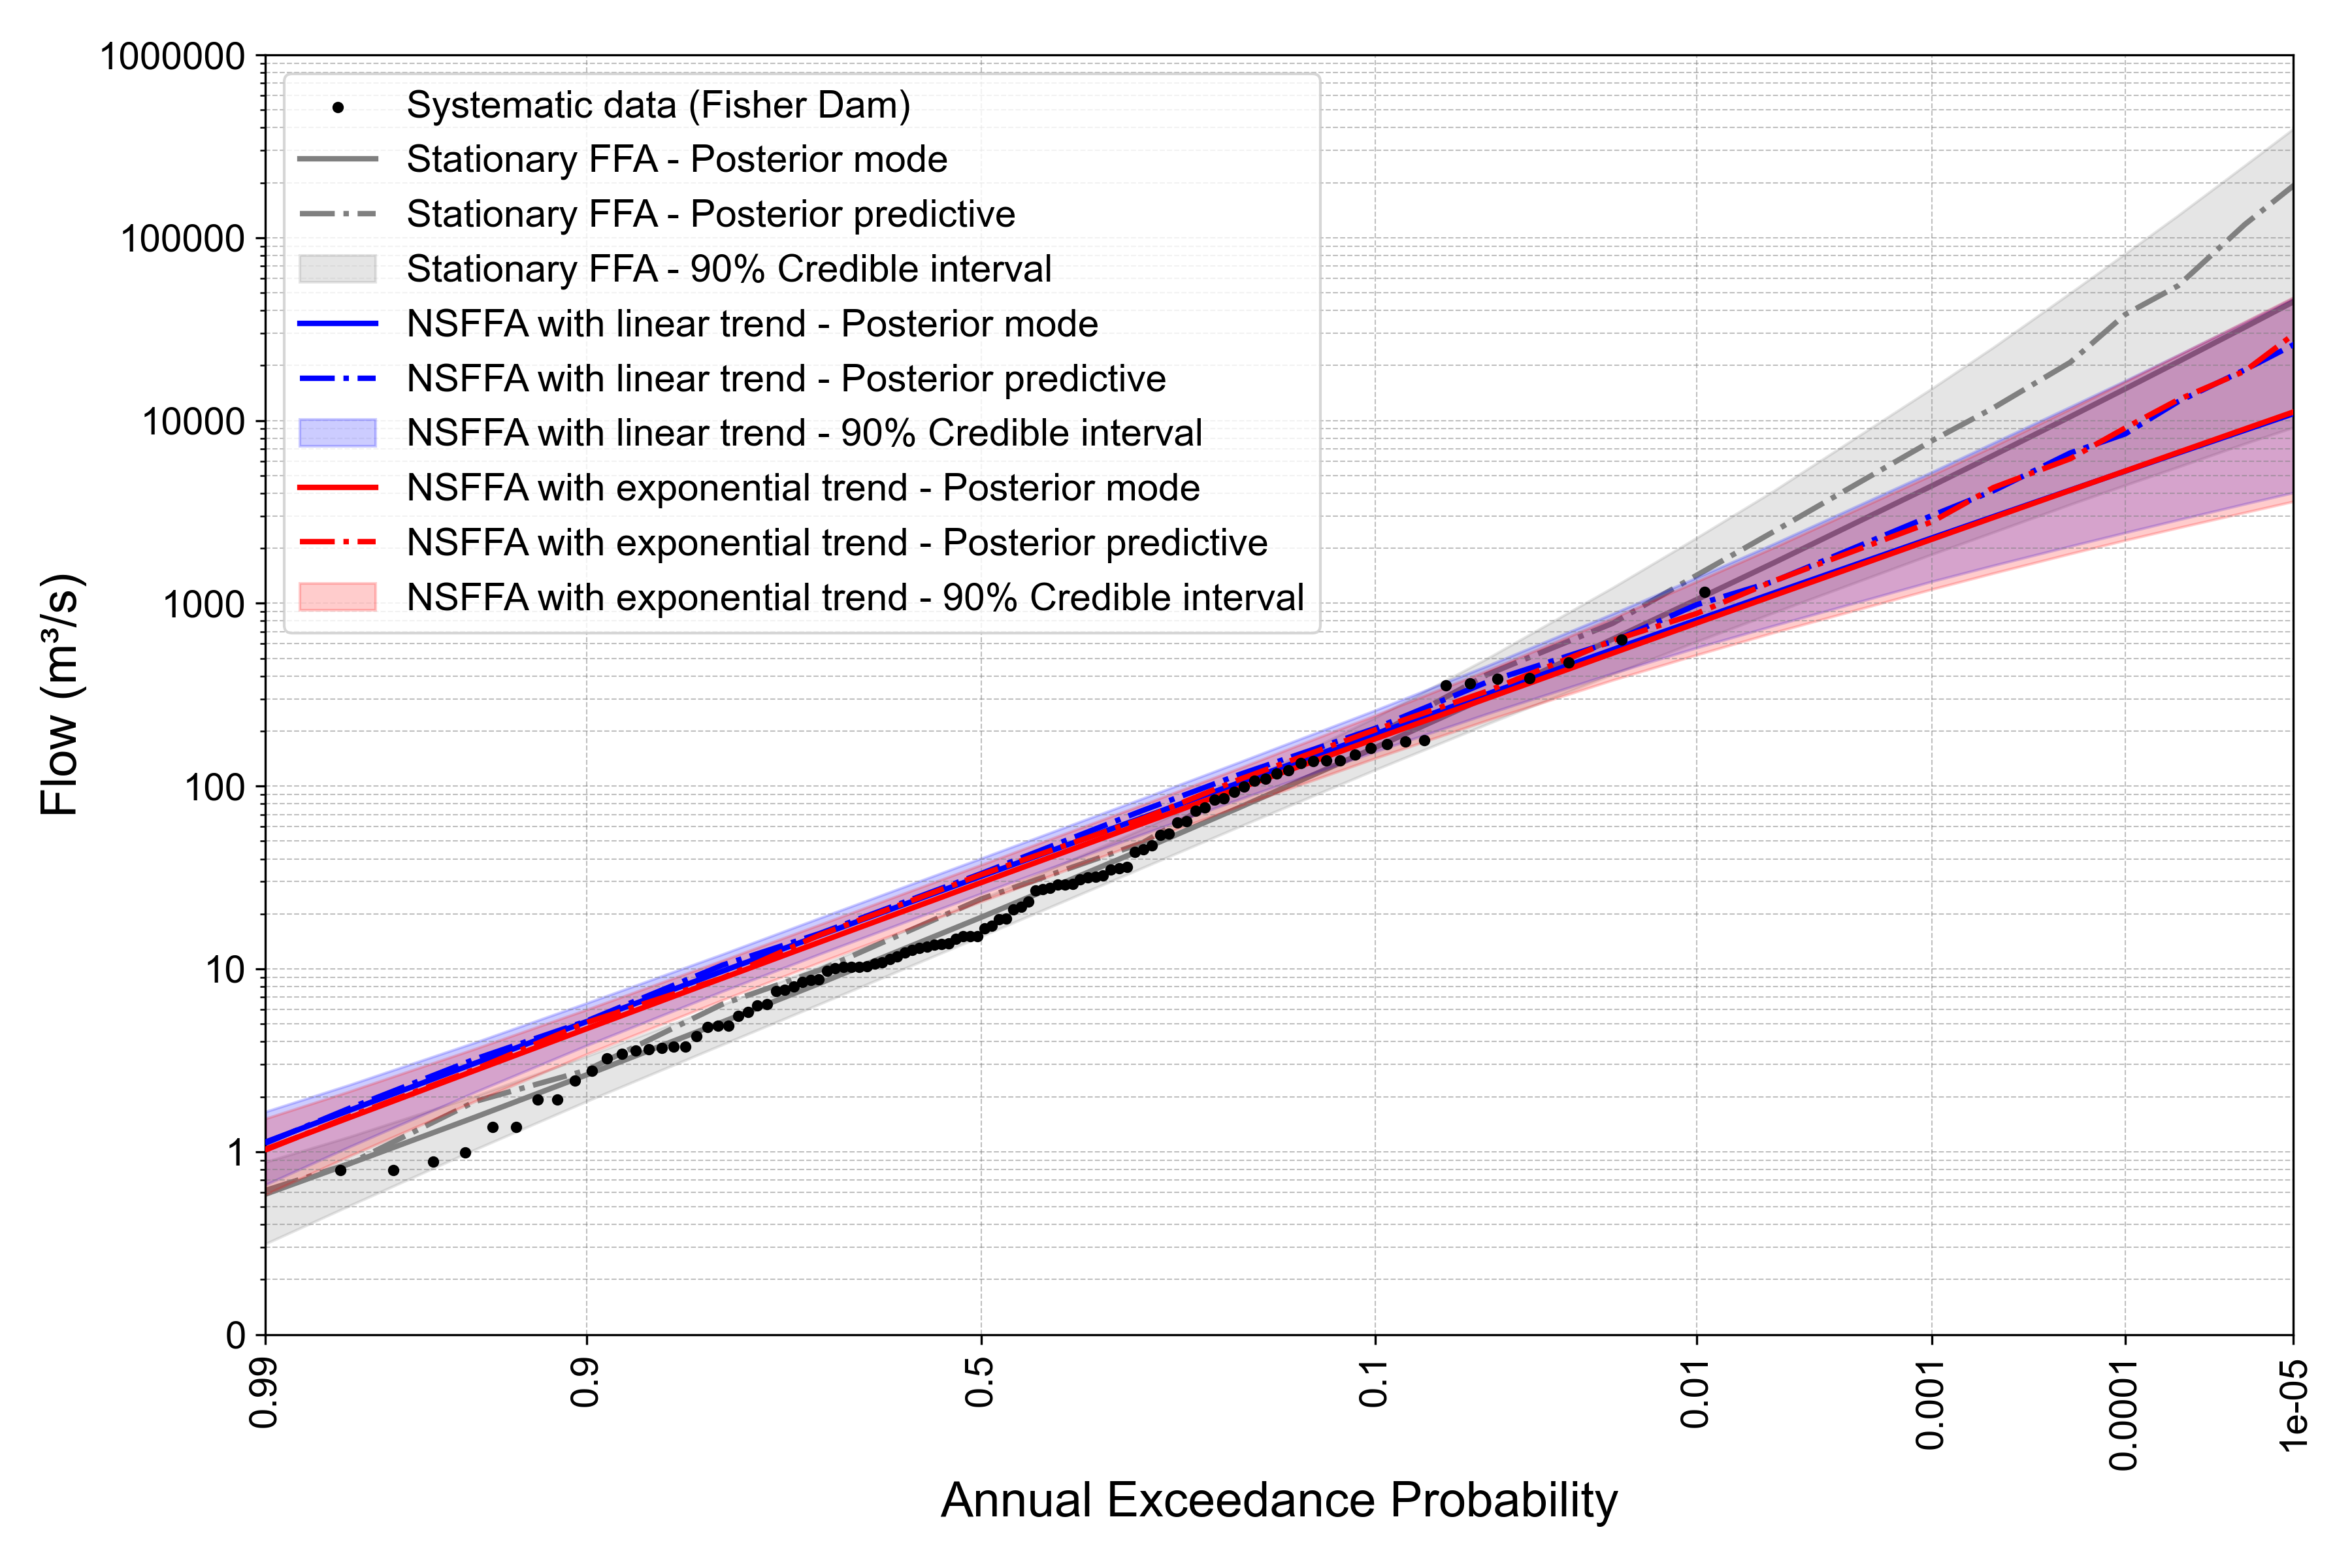
\includegraphics[width=1\linewidth]{_plots/OCD_bayesian_flood_quantiles_lp3_nonstationary.png}    
    \caption{Flood frequency curves derived from stationary FFA and NSFFA models (TI = 1949) compared against observed data for the Fisher Dam dataset. }

    \label{fig:OCD_bayesian_flood_quantiles_lp3_nonstationary}
\end{figure*}

\begin{figure*}[ht!]
    \centering
    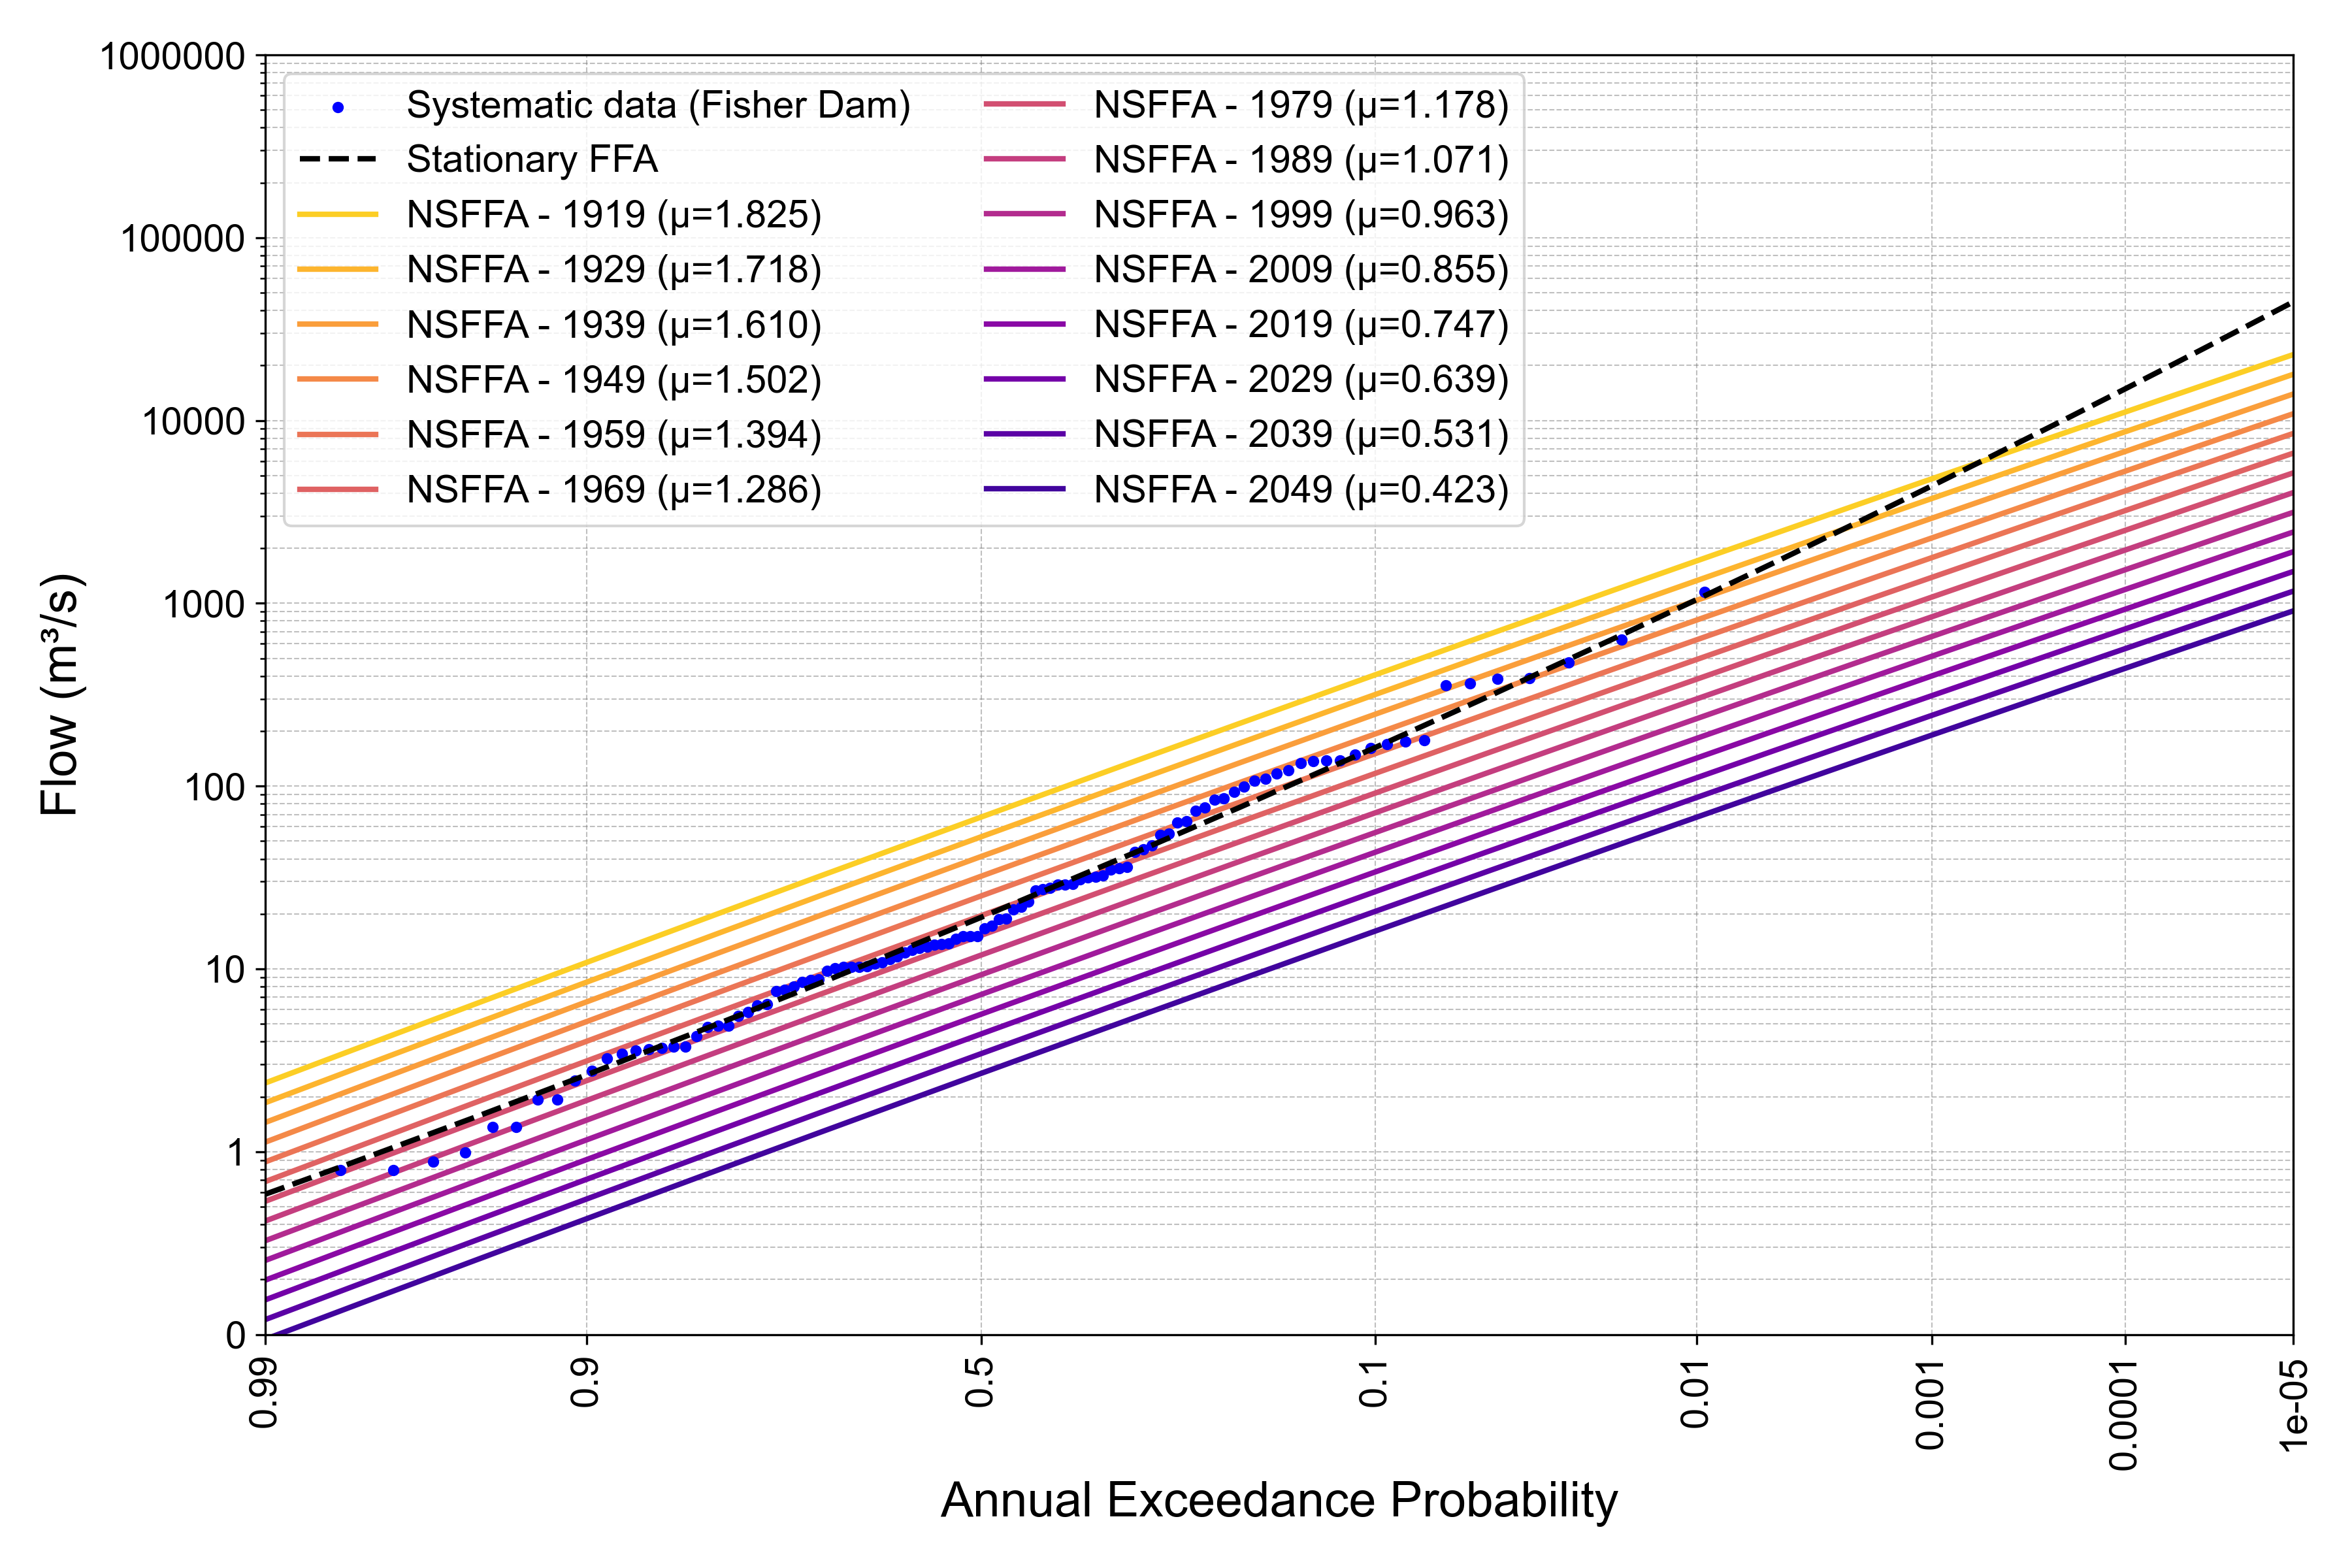
\includegraphics[width=1\linewidth]{_plots/OCD_bayesian_flood_quantiles_lp3_linear_mu_TI.png}
    \caption{Impact of time index selection on flood frequency curves derived from the linear trend NSFFA model compared against stationary FFA and observed data for the Fisher Dam dataset.}
    \label{fig:OCD_bayesian_flood_quantiles_lp3_linear_mu_TI}
\end{figure*}
 

\section{Conclusion}
This study demonstrated the application of a Bayesian computational framework in flood frequency hydrology. We utilized an adaptive DE-MCzS algorithm for the MCMC process. The approach was validated through two case studies using publicly available datasets, with results verified against BestFit, a leading hydrological software developed by USACE. 

The stationary analysis of the Harricana River dataset evaluated the efficiency and robustness of the adaptive DE-MCzS algorithm while also demonstrating the advantages over MLE. The computed posterior mode, posterior predictive distributions, and credible intervals aligned exceptionally well with BestFit when the same noise term was applied. The non-stationary analysis of the O.C. Fisher Dam dataset further emphasized the Bayesian approach’s capability in modeling temporal dynamics as a time-variant property of the location parameter. Both stationary and non-stationary models (NSFFA with linear and exponential trends) produced results closely aligned with BestFit. Sensitivity analysis on the TI selection revealed the significant influence of temporal parameters on flood frequency curves. 

By incorporating prior knowledge and explicitly quantifying uncertainty, the Bayesian approach proved to be a powerful tool for managing flood risks, especially in the context of data scarcity, increasing uncertainties, and the evolving impacts of climate change. This integration of probabilistic reasoning with hydrological modeling enhances decision-making processes, offering robust solutions to the complex challenges faced in flood risk assessment and management. 

\section*{Open Data Statement}
All data and code used in this study are openly available to ensure transparency, reproducibility, and to encourage further research. The dataset and scripts supporting the findings of this study have been archived and can be accessed via the project's GitHub repository at: \href{https://github.com/Wang-Yanni/Bayesian_FFA}{https://github.com/Wang-Yanni/Bayesian\_FFA}. For additional inquiries, please contact the corresponding author.


\section*{Acknowledgment}
We gratefully acknowledge Cole Haden Smith from the USACE-RMC for open-sourcing the Numerics library. This resource was instrumental in decoding the DE-MCzS sampler employed in this study. We also deeply appreciate his prompt and insightful responses to our queries regarding posterior calculations, which greatly enhanced the clarity and robustness of our Bayesian analyses. 
 

\bibliographystyle{plain}
\bibliography{_Reference}
\newpage
\section*{Appendix A - Harricana River dataset}

\renewcommand{\arraystretch}{1.2}
\begin{table}[H]
\centering
\caption{Flow measurements (CMS) by year for the Harricana River dataset.}
\begin{tabular}{l c | l c | l c}
\hline
\textbf{Year} & \textbf{Flow} & \textbf{Year} & \textbf{Flow} & \textbf{Year} & \textbf{Flow} \\ \hline
1915 & 122   & 1938 & 240   & 1961 & 125   \\
1916 & 244   & 1939 & 230   & 1962 & 166   \\
1917 & 214   & 1940 & 192   & 1963 & 99  \\
1918 & 173   & 1941 & 195   & 1964 & 202   \\
1919 & 229   & 1942 & 172   & 1965 & 230   \\
1920 & 156   & 1943 & 173   & 1966 & 158   \\
1921 & 212   & 1944 & 172   & 1967 & 262   \\
1922 & 263   & 1945 & 153   & 1968 & 154   \\
1923 & 146   & 1946 & 142   & 1969 & 164   \\
1924 & 183   & 1947 & 317   & 1970 & 182   \\
1925 & 161   & 1948 & 161   & 1971 & 164   \\
1926 & 205   & 1949 & 201   & 1972 & 183   \\
1927 & 135   & 1950 & 204   & 1973 & 171   \\
1928 & 331   & 1951 & 194   & 1974 & 250   \\
1929 & 225   & 1952 & 164   & 1975 & 184   \\
1930 & 174   & 1953 & 183   & 1976 & 205   \\
1931 & 99  & 1954 & 161   & 1977 & 237   \\
1932 & 149   & 1955 & 167   & 1978 & 177   \\
1933 & 238   & 1956 & 179   & 1979 & 239   \\
1934 & 262   & 1957 & 185   & 1980 & 187   \\
1935 & 132   & 1958 & 117   & 1981 & 180   \\
1936 & 235   & 1959 & 192   & 1982 & 173   \\
1937 & 216   & 1960 & 337   & 1983 & 174   \\ \hline
\end{tabular}
\label{table:HRA_flows}
\end{table}


\section*{Appendix B - Fisher Dam dataset}

\renewcommand{\arraystretch}{1.2}
\begin{table}[H]
\centering
\caption{Flow measurements (CMS) by year for the Fisher Dam dataset (rounded to integers).}
\begin{tabular}{l c | l c | l c}
\hline
\textbf{Year} & \textbf{Flow} & \textbf{Year} & \textbf{Flow} & \textbf{Year} & \textbf{Flow} \\ \hline
1916 & 14   & 1943 & 6    & 1970 & 1    \\
1917 & 35   & 1944 & 15   & 1971 & 28   \\
1918 & 110  & 1945 & 366  & 1972 & 12   \\
1919 & 148  & 1946 & 5    & 1973 & 19   \\
1920 & 17   & 1947 & 138  & 1974 & 178  \\
1921 & 3    & 1948 & 473  & 1975 & 31   \\
1922 & 357  & 1949 & 134  & 1976 & 2    \\
1923 & 11   & 1950 & 44   & 1977 & 9    \\
1924 & 64   & 1951 & 23   & 1978 & 33   \\
1925 & 388  & 1952 & 6    & 1979 & 3    \\
1926 & 122  & 1953 & 137  & 1980 & 86   \\
1927 & 32   & 1954 & 55   & 1981 & 22   \\
1928 & 139  & 1955 & 13   & 1982 & 12   \\
1929 & 54   & 1956 & 35   & 1983 & 15   \\
1930 & 169  & 1957 & 632  & 1984 & 4    \\
1931 & 11   & 1958 & 10   & 1985 & 8    \\
1932 & 175  & 1959 & 84   & 1986 & 162  \\
1933 & 1    & 1960 & 8    & 1987 & 15   \\
1934 & 76   & 1961 & 99   & 1988 & 14   \\
1935 & 387  & 1962 & 6    & 1989 & 10   \\
1936 & 1149 & 1963 & 14   & 1990 & 10   \\
1937 & 117  & 1964 & 47   & 1991 & 8    \\
1938 & 93   & 1965 & 29   & 1992 & 15   \\
1939 & 5    & 1966 & 29   & 1993 & 2    \\
1940 & 27   & 1967 & 9    & 1994 & 11   \\
1941 & 73   & 1968 & 19   & 1995 & 4    \\
1942 & 10   & 1969 & 4    & 1996 & 10   \\ \hline
\end{tabular}
\label{table:OCD_flows}
\end{table}

\newpage
\section*{Appendix C - Fisher Dam: NSFFA Verification Results}

\begin{figure}[H]
    \centering
    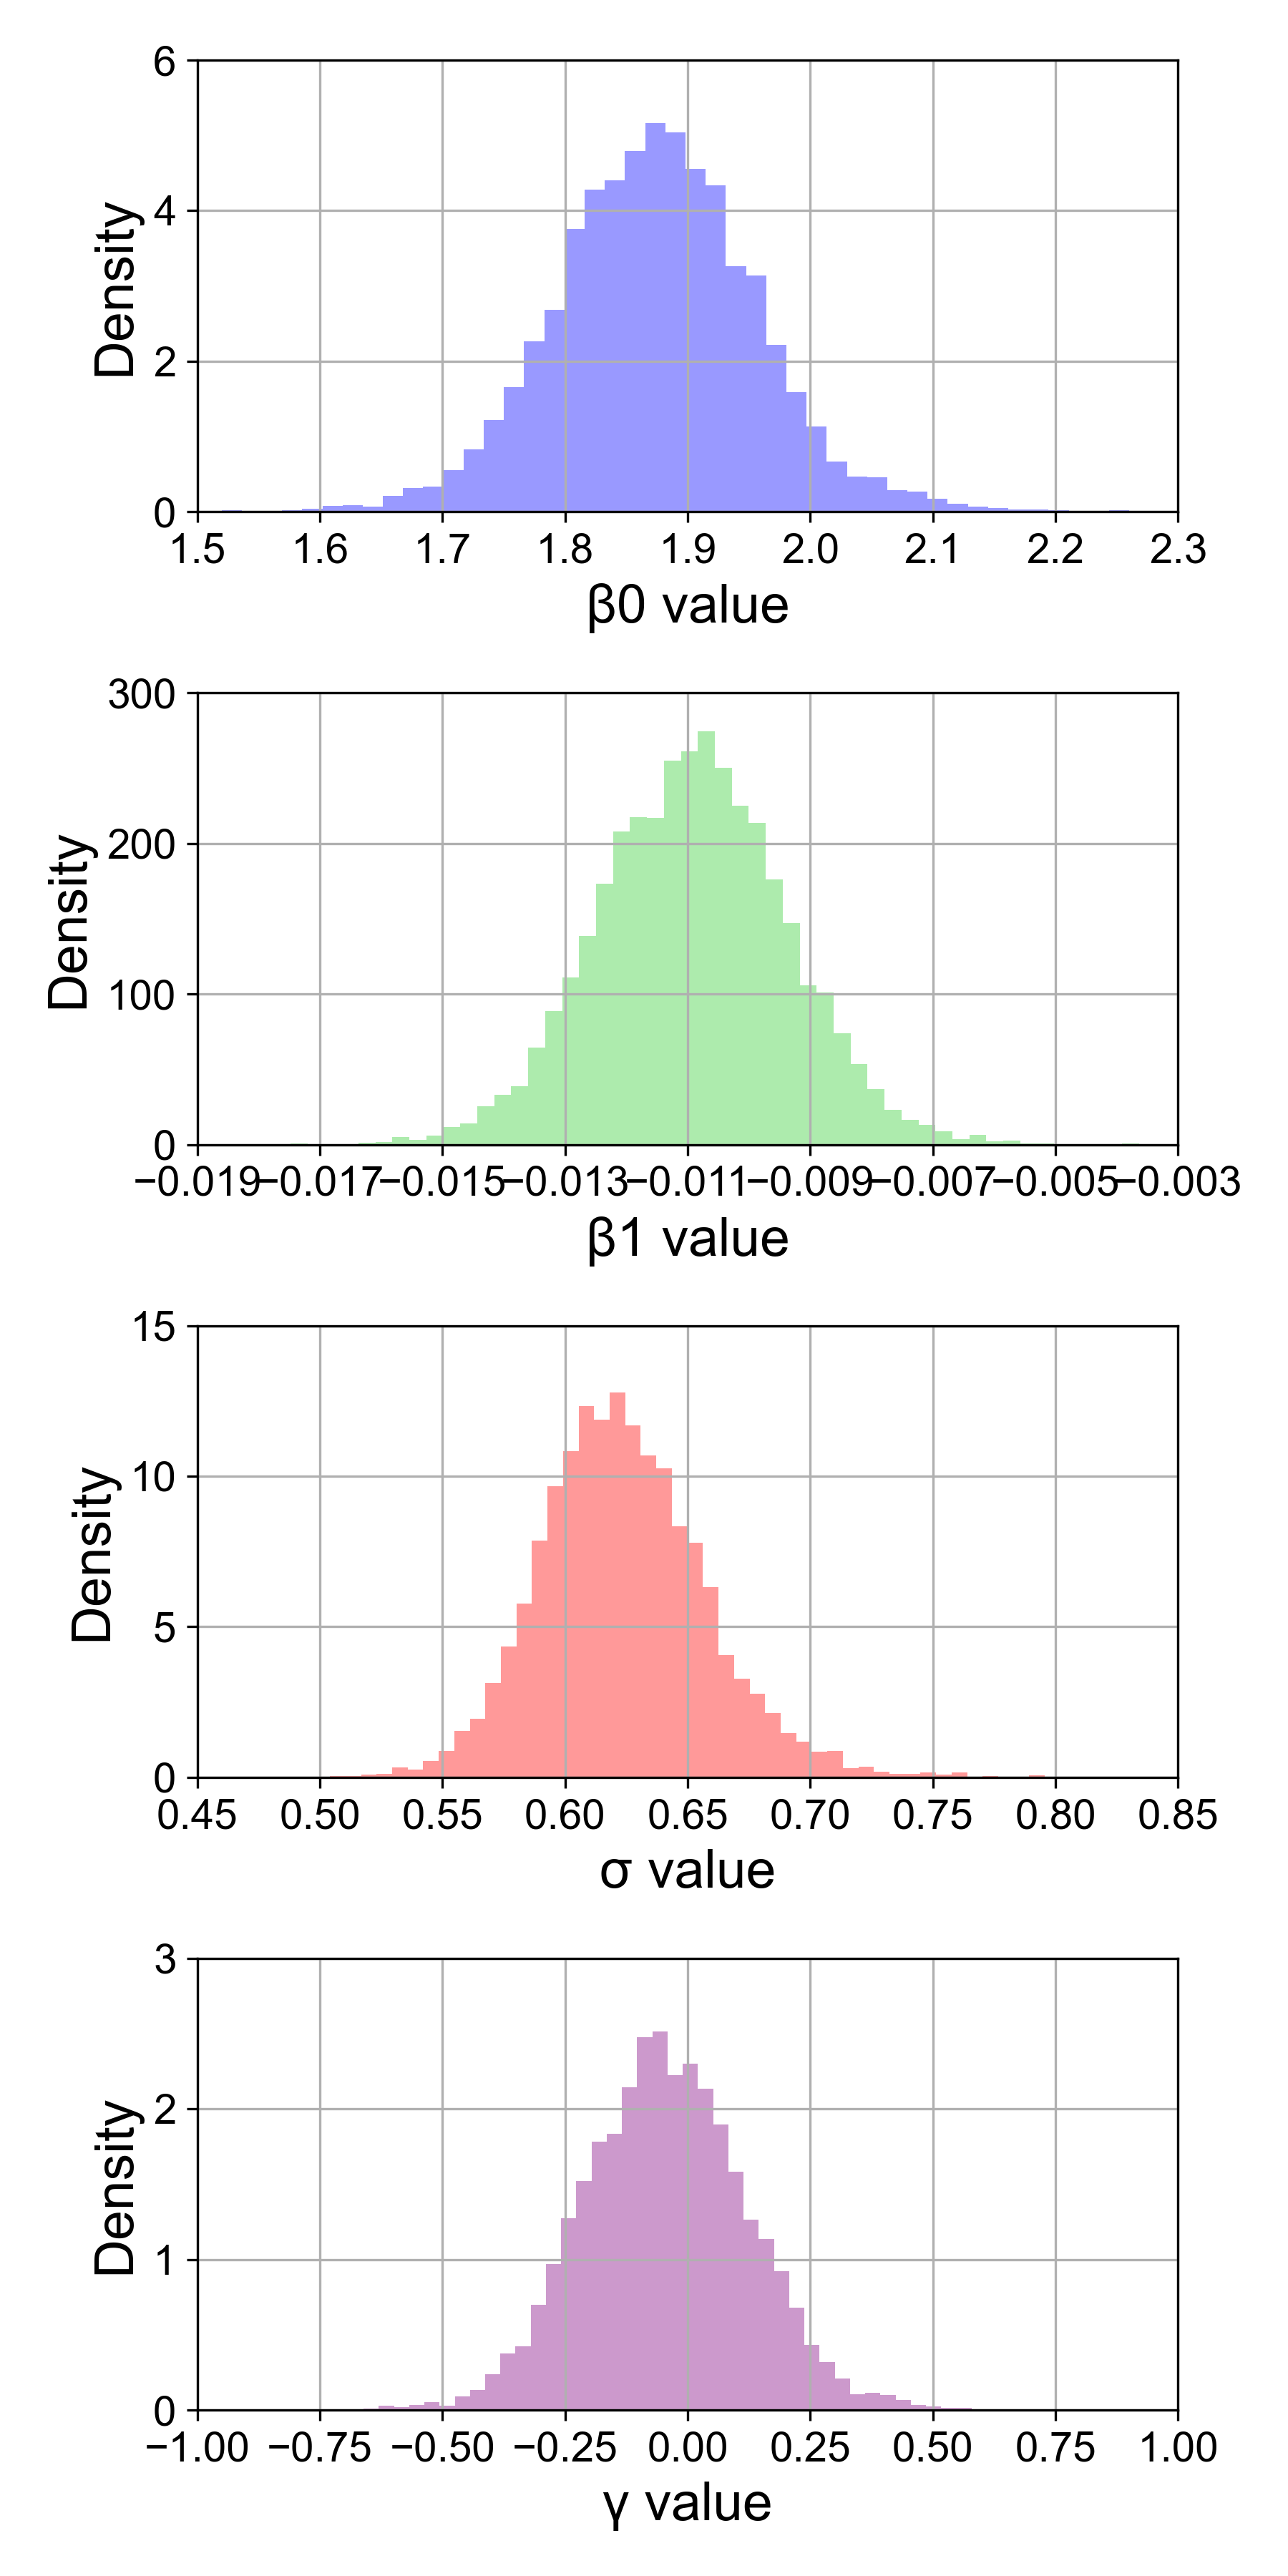
\includegraphics[width=1\linewidth]{_plots/OCD_linear_mu_posterior_marginal_lp3.png}
    \caption{Posterior marginal distributions of LP3 distribution parameters for the NSFFA model with linear trend, derived from the Fisher Dam dataset.}
    \label{fig:OCD_linear_mu_posterior_marginal_lp3}
\end{figure}

\begin{figure}[H]
    \centering
    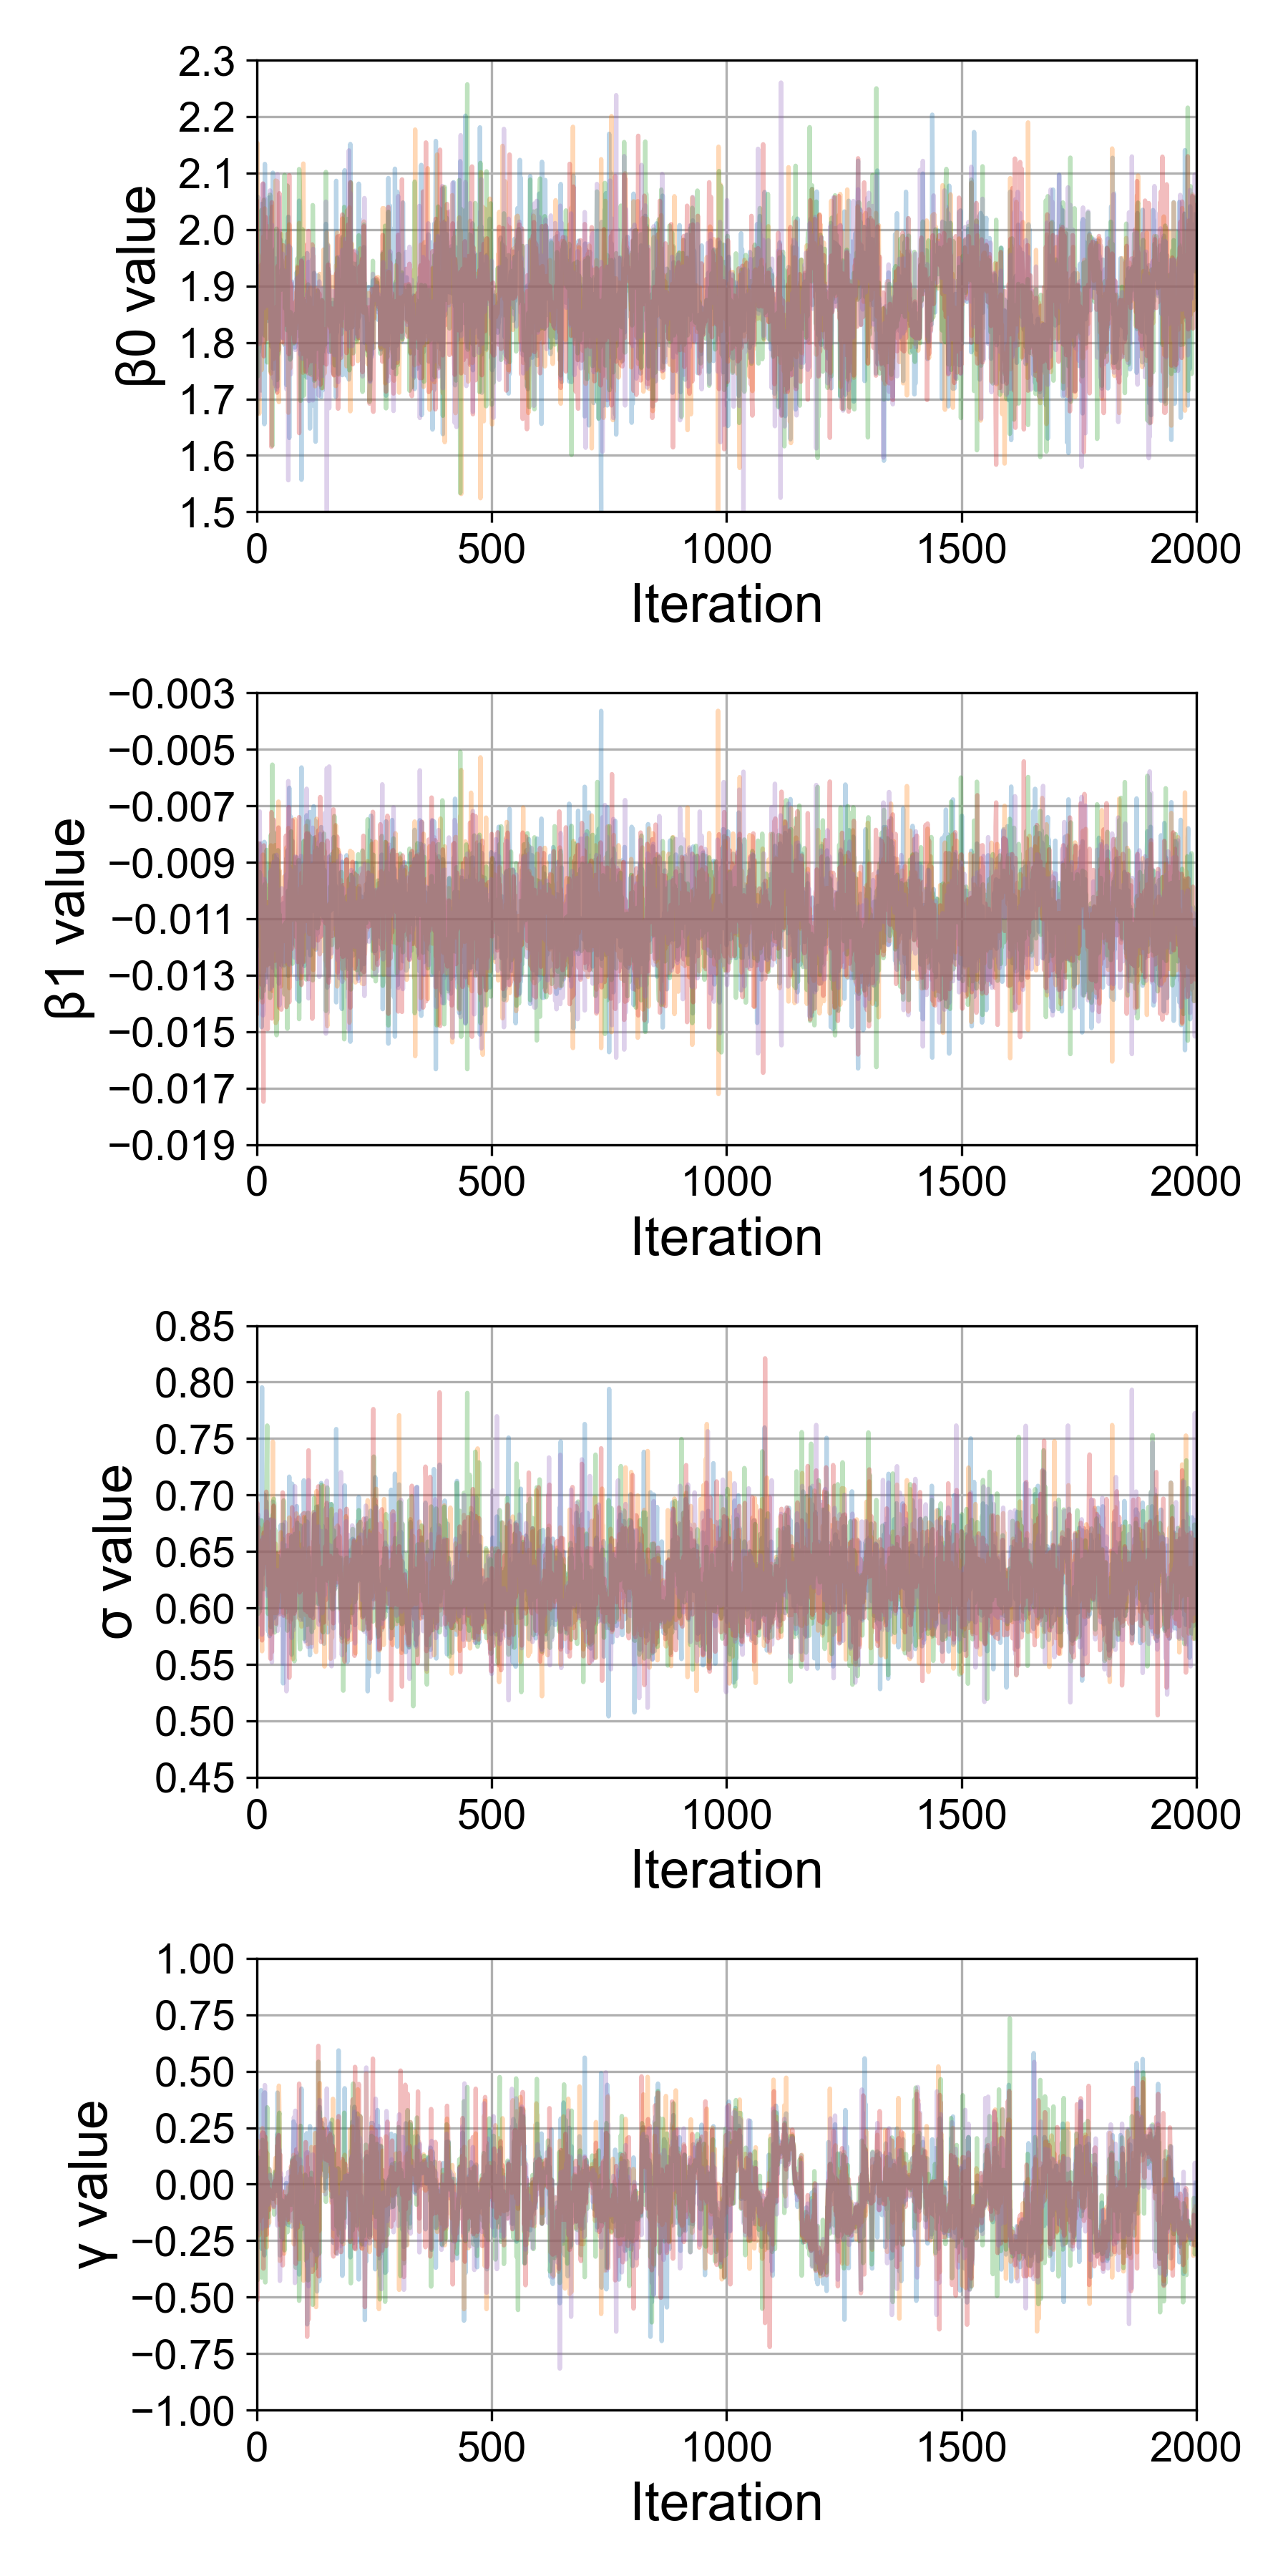
\includegraphics[width=1\linewidth]{_plots/OCD_linear_mu_posterior_trace_lp3.png}
    \caption{Trace plots of LP3 distribution parameters for the NSFFA model with linear trend, derived from the Fisher Dam dataset.}
    \label{fig:OCD_linear_mu_posterior_trace_lp3}
\end{figure}

\newpage
\begin{figure}[H]
    \centering
    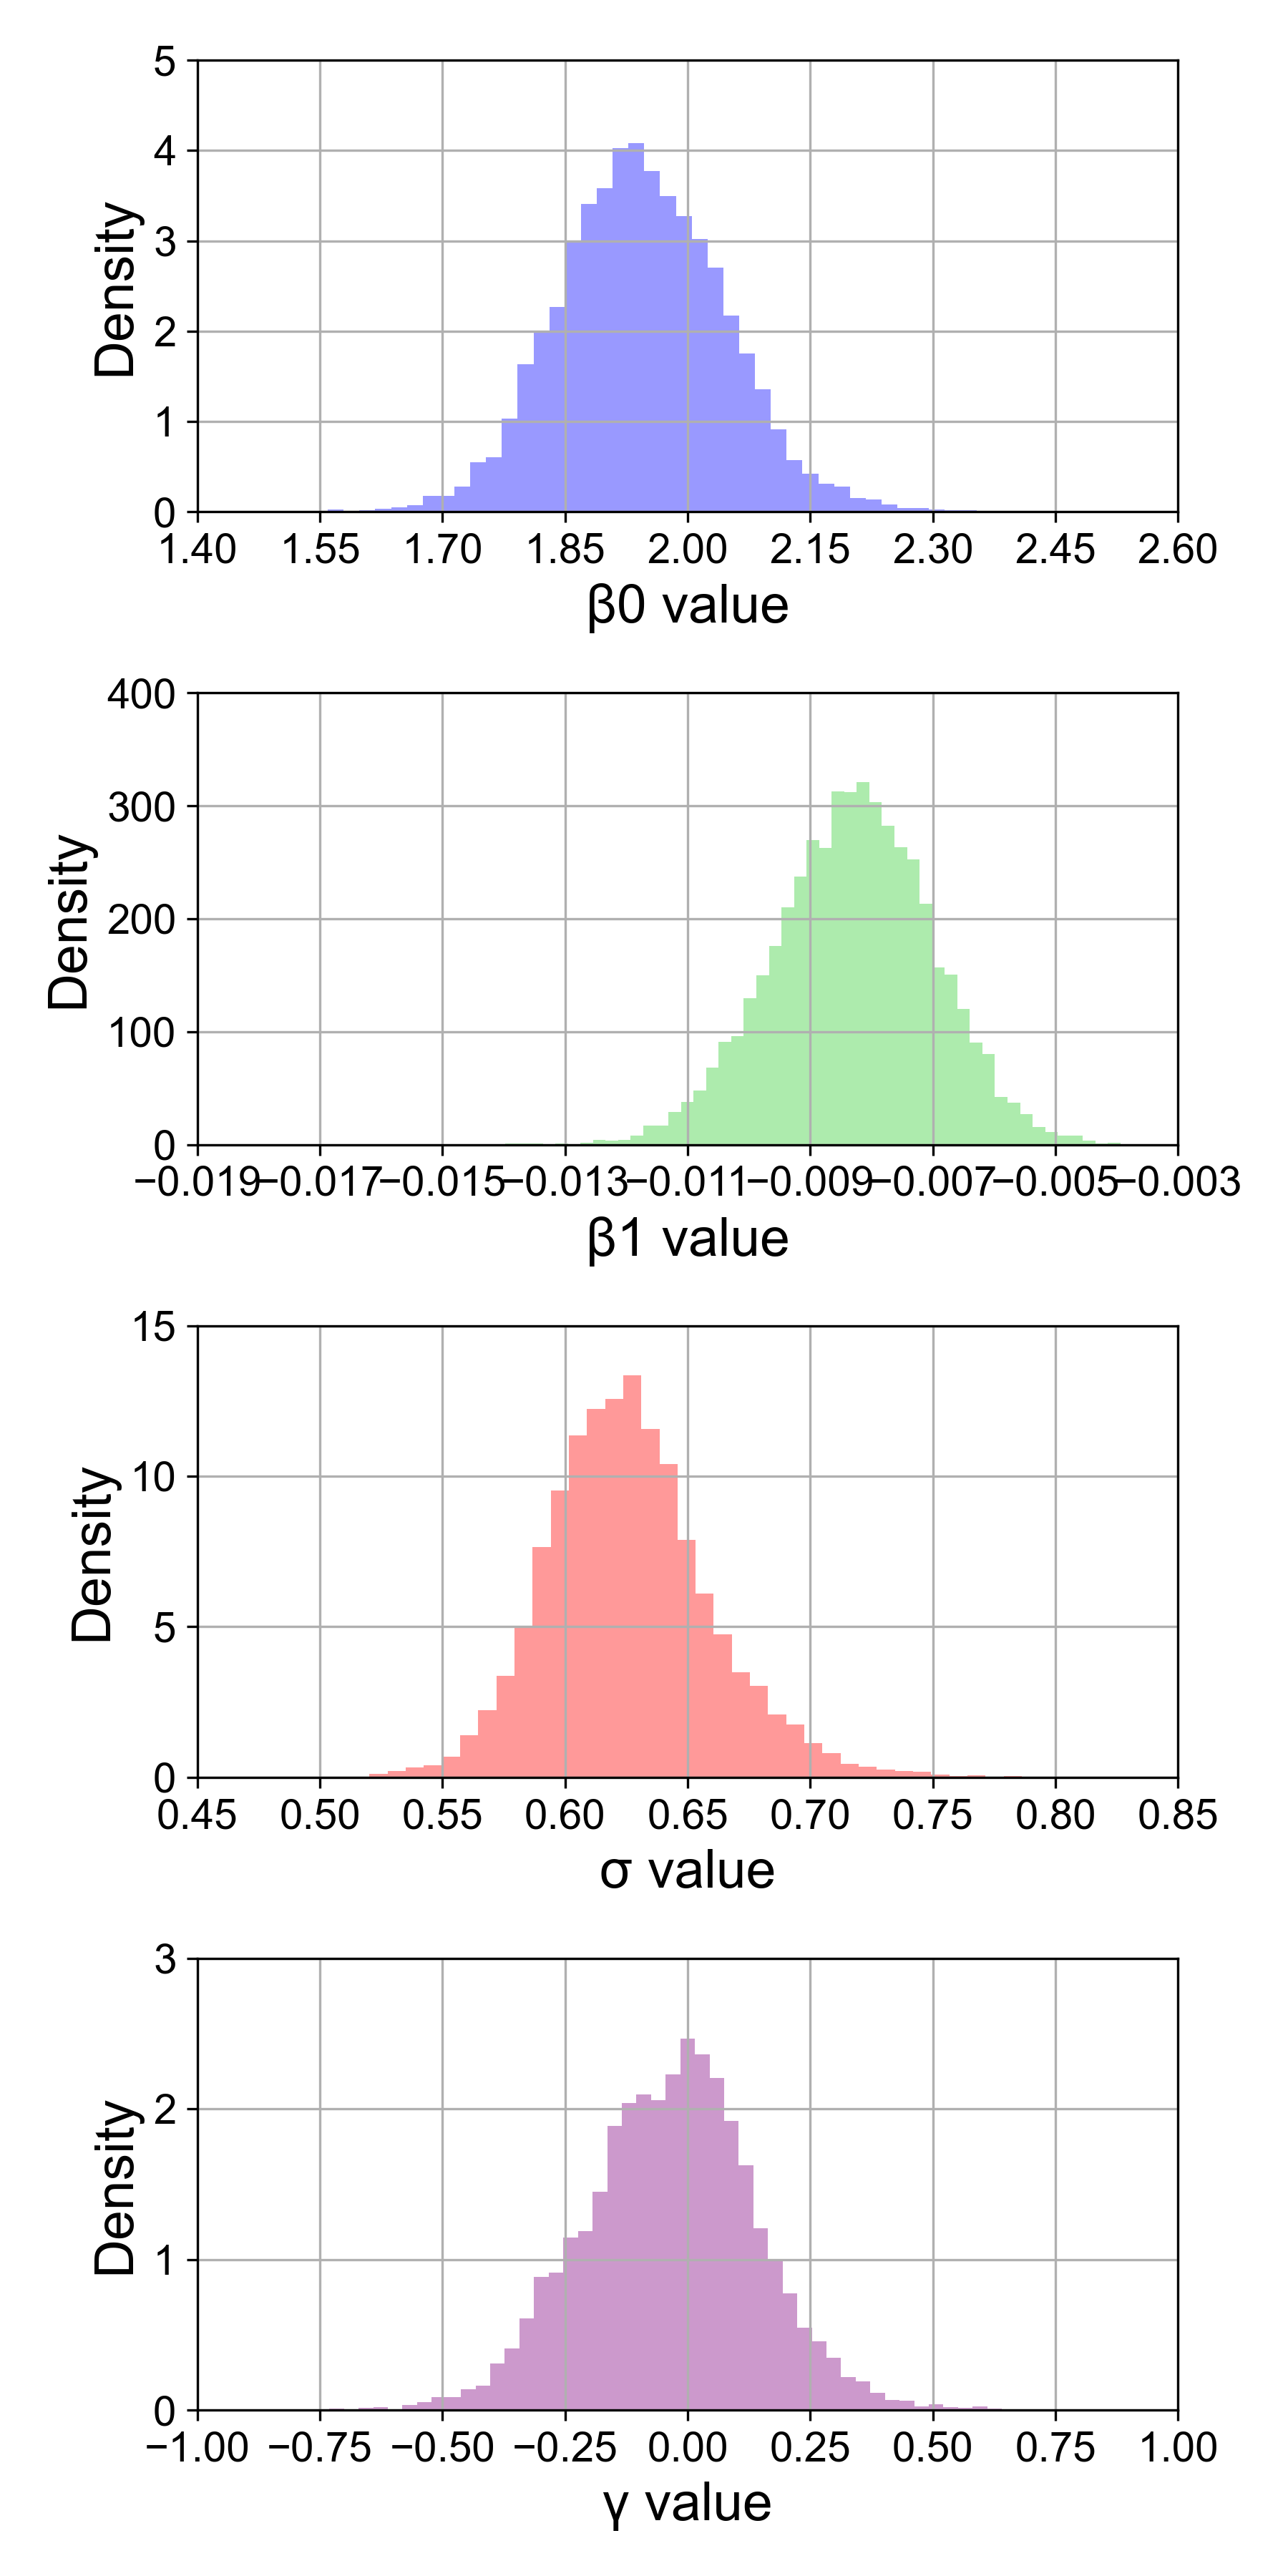
\includegraphics[width=1\linewidth]{_plots/OCD_exponential_mu_posterior_marginal_lp3.png}
    \caption{Posterior marginal distributions of LP3 distribution parameters for the NSFFA model with exponential trend, derived from the Fisher Dam dataset.}
    \label{fig:OCD_exponential_mu_posterior_marginal_lp3}
\end{figure}

\begin{figure}[H]
    \centering
    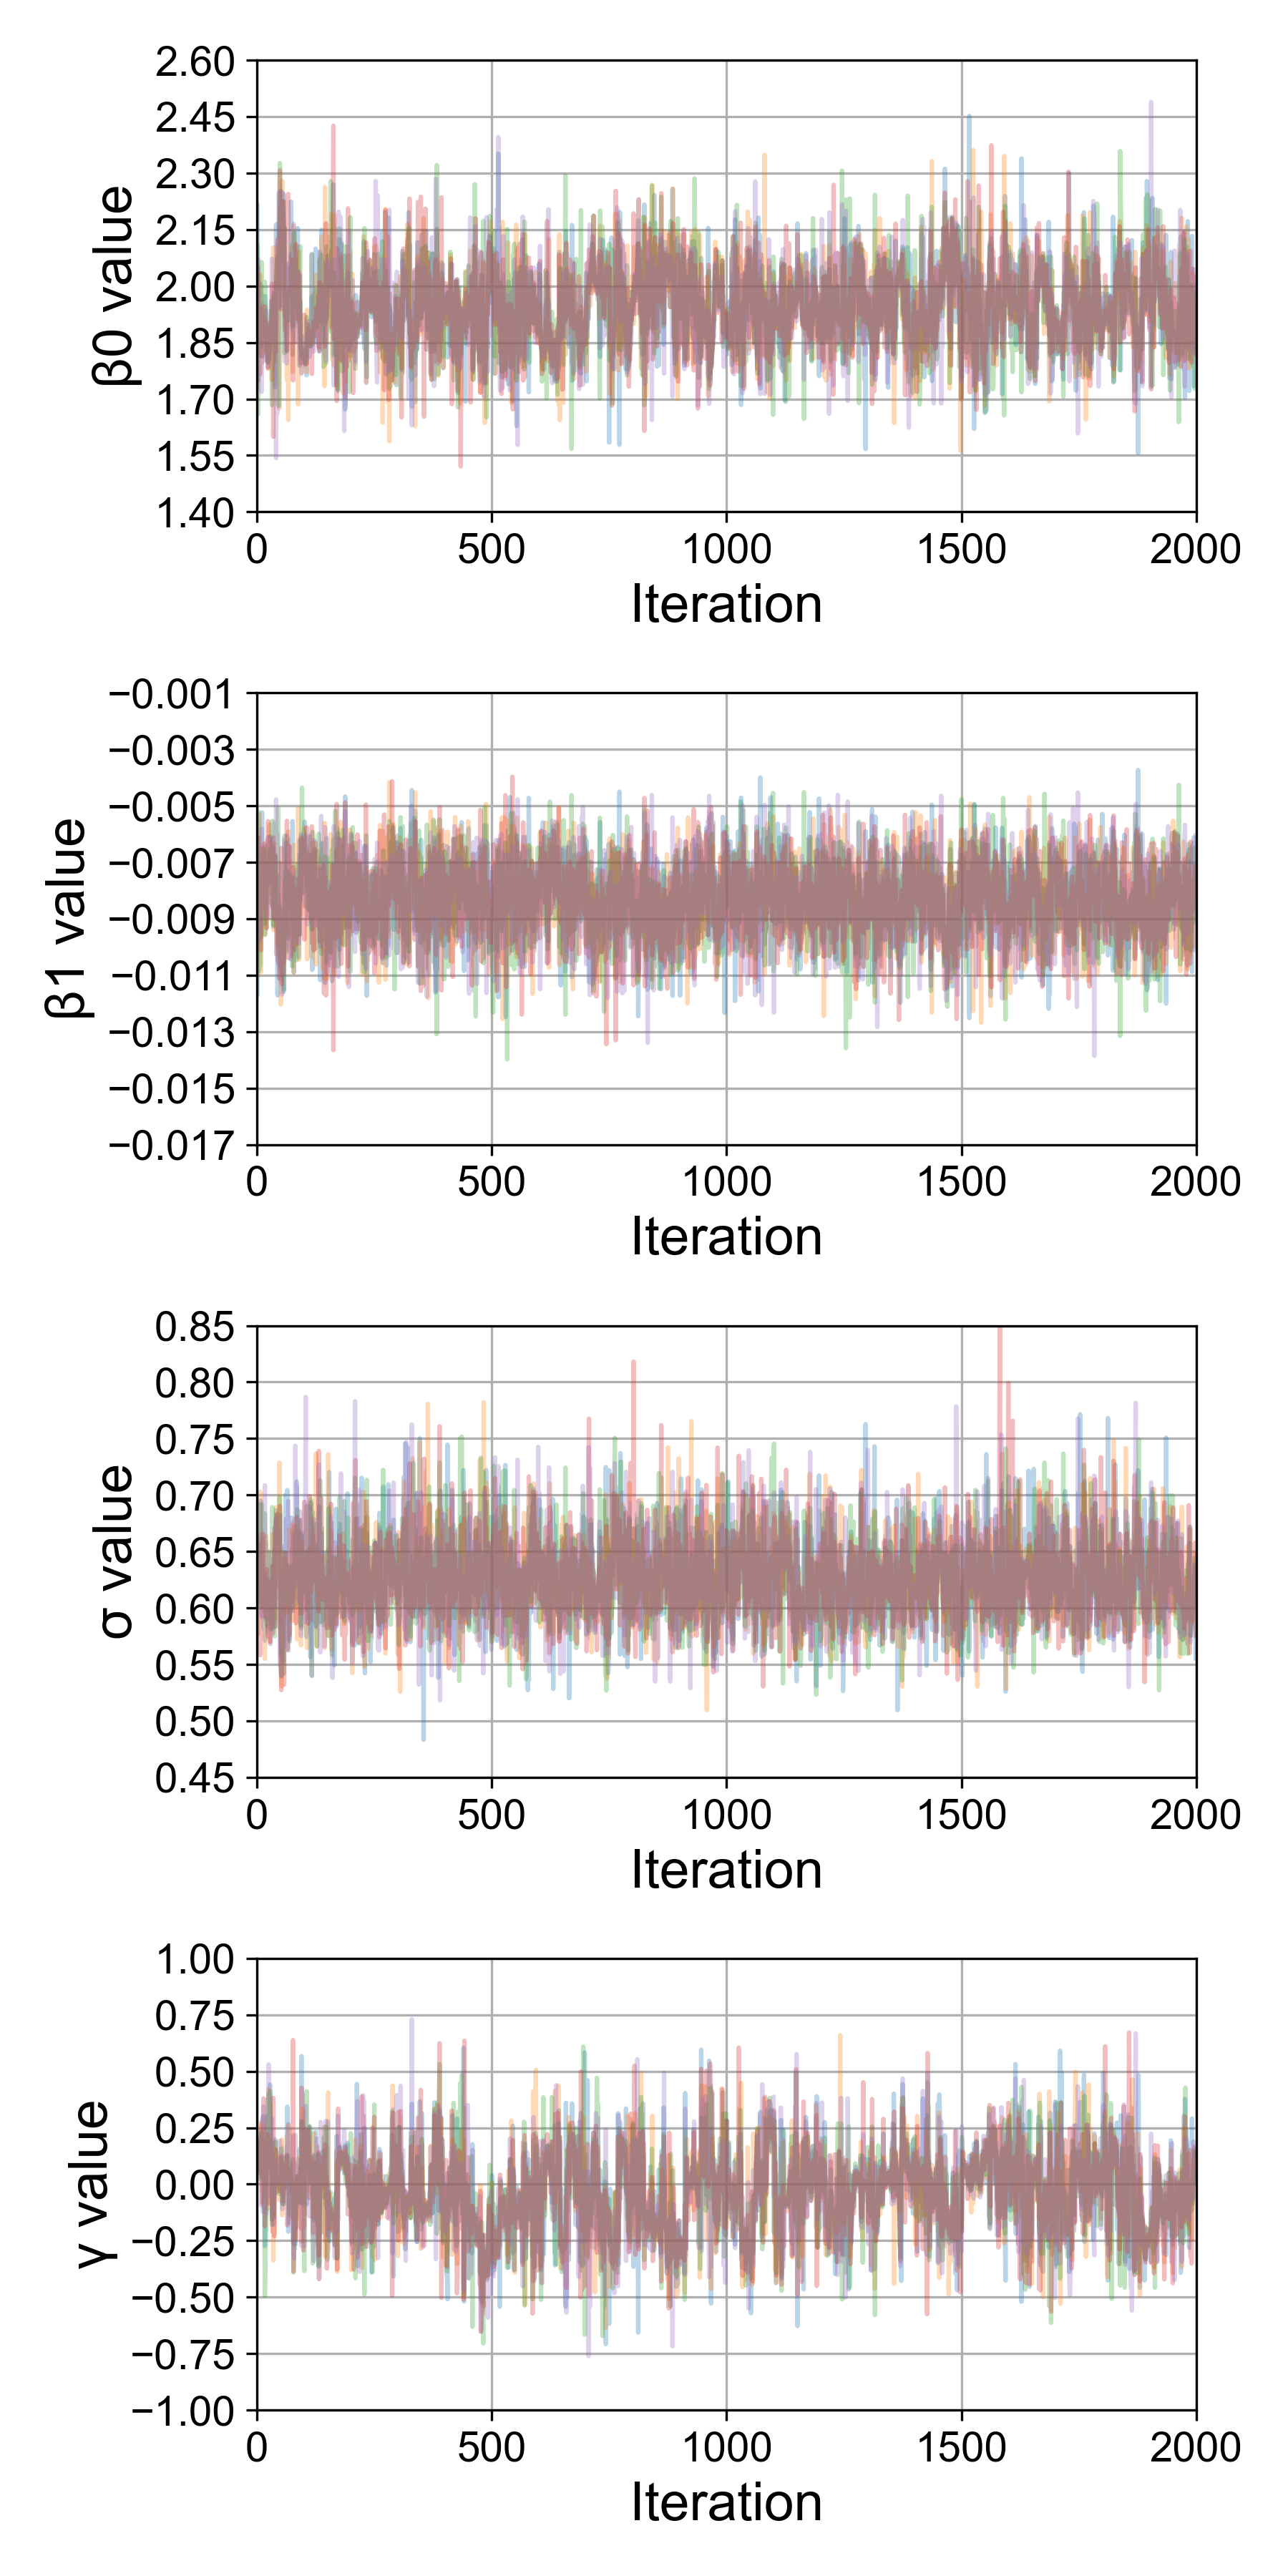
\includegraphics[width=1\linewidth]{_plots/OCD_exponential_mu_posterior_trace_lp3.png}
    \caption{Trace plots of LP3 distribution parameters for the NSFFA model with exponential trend, derived from the Fisher Dam dataset.}
    \label{fig:OCD_exponential_mu_posterior_trace_lp3}
\end{figure}

\newpage
\begin{figure*}[htp]
    \centering
    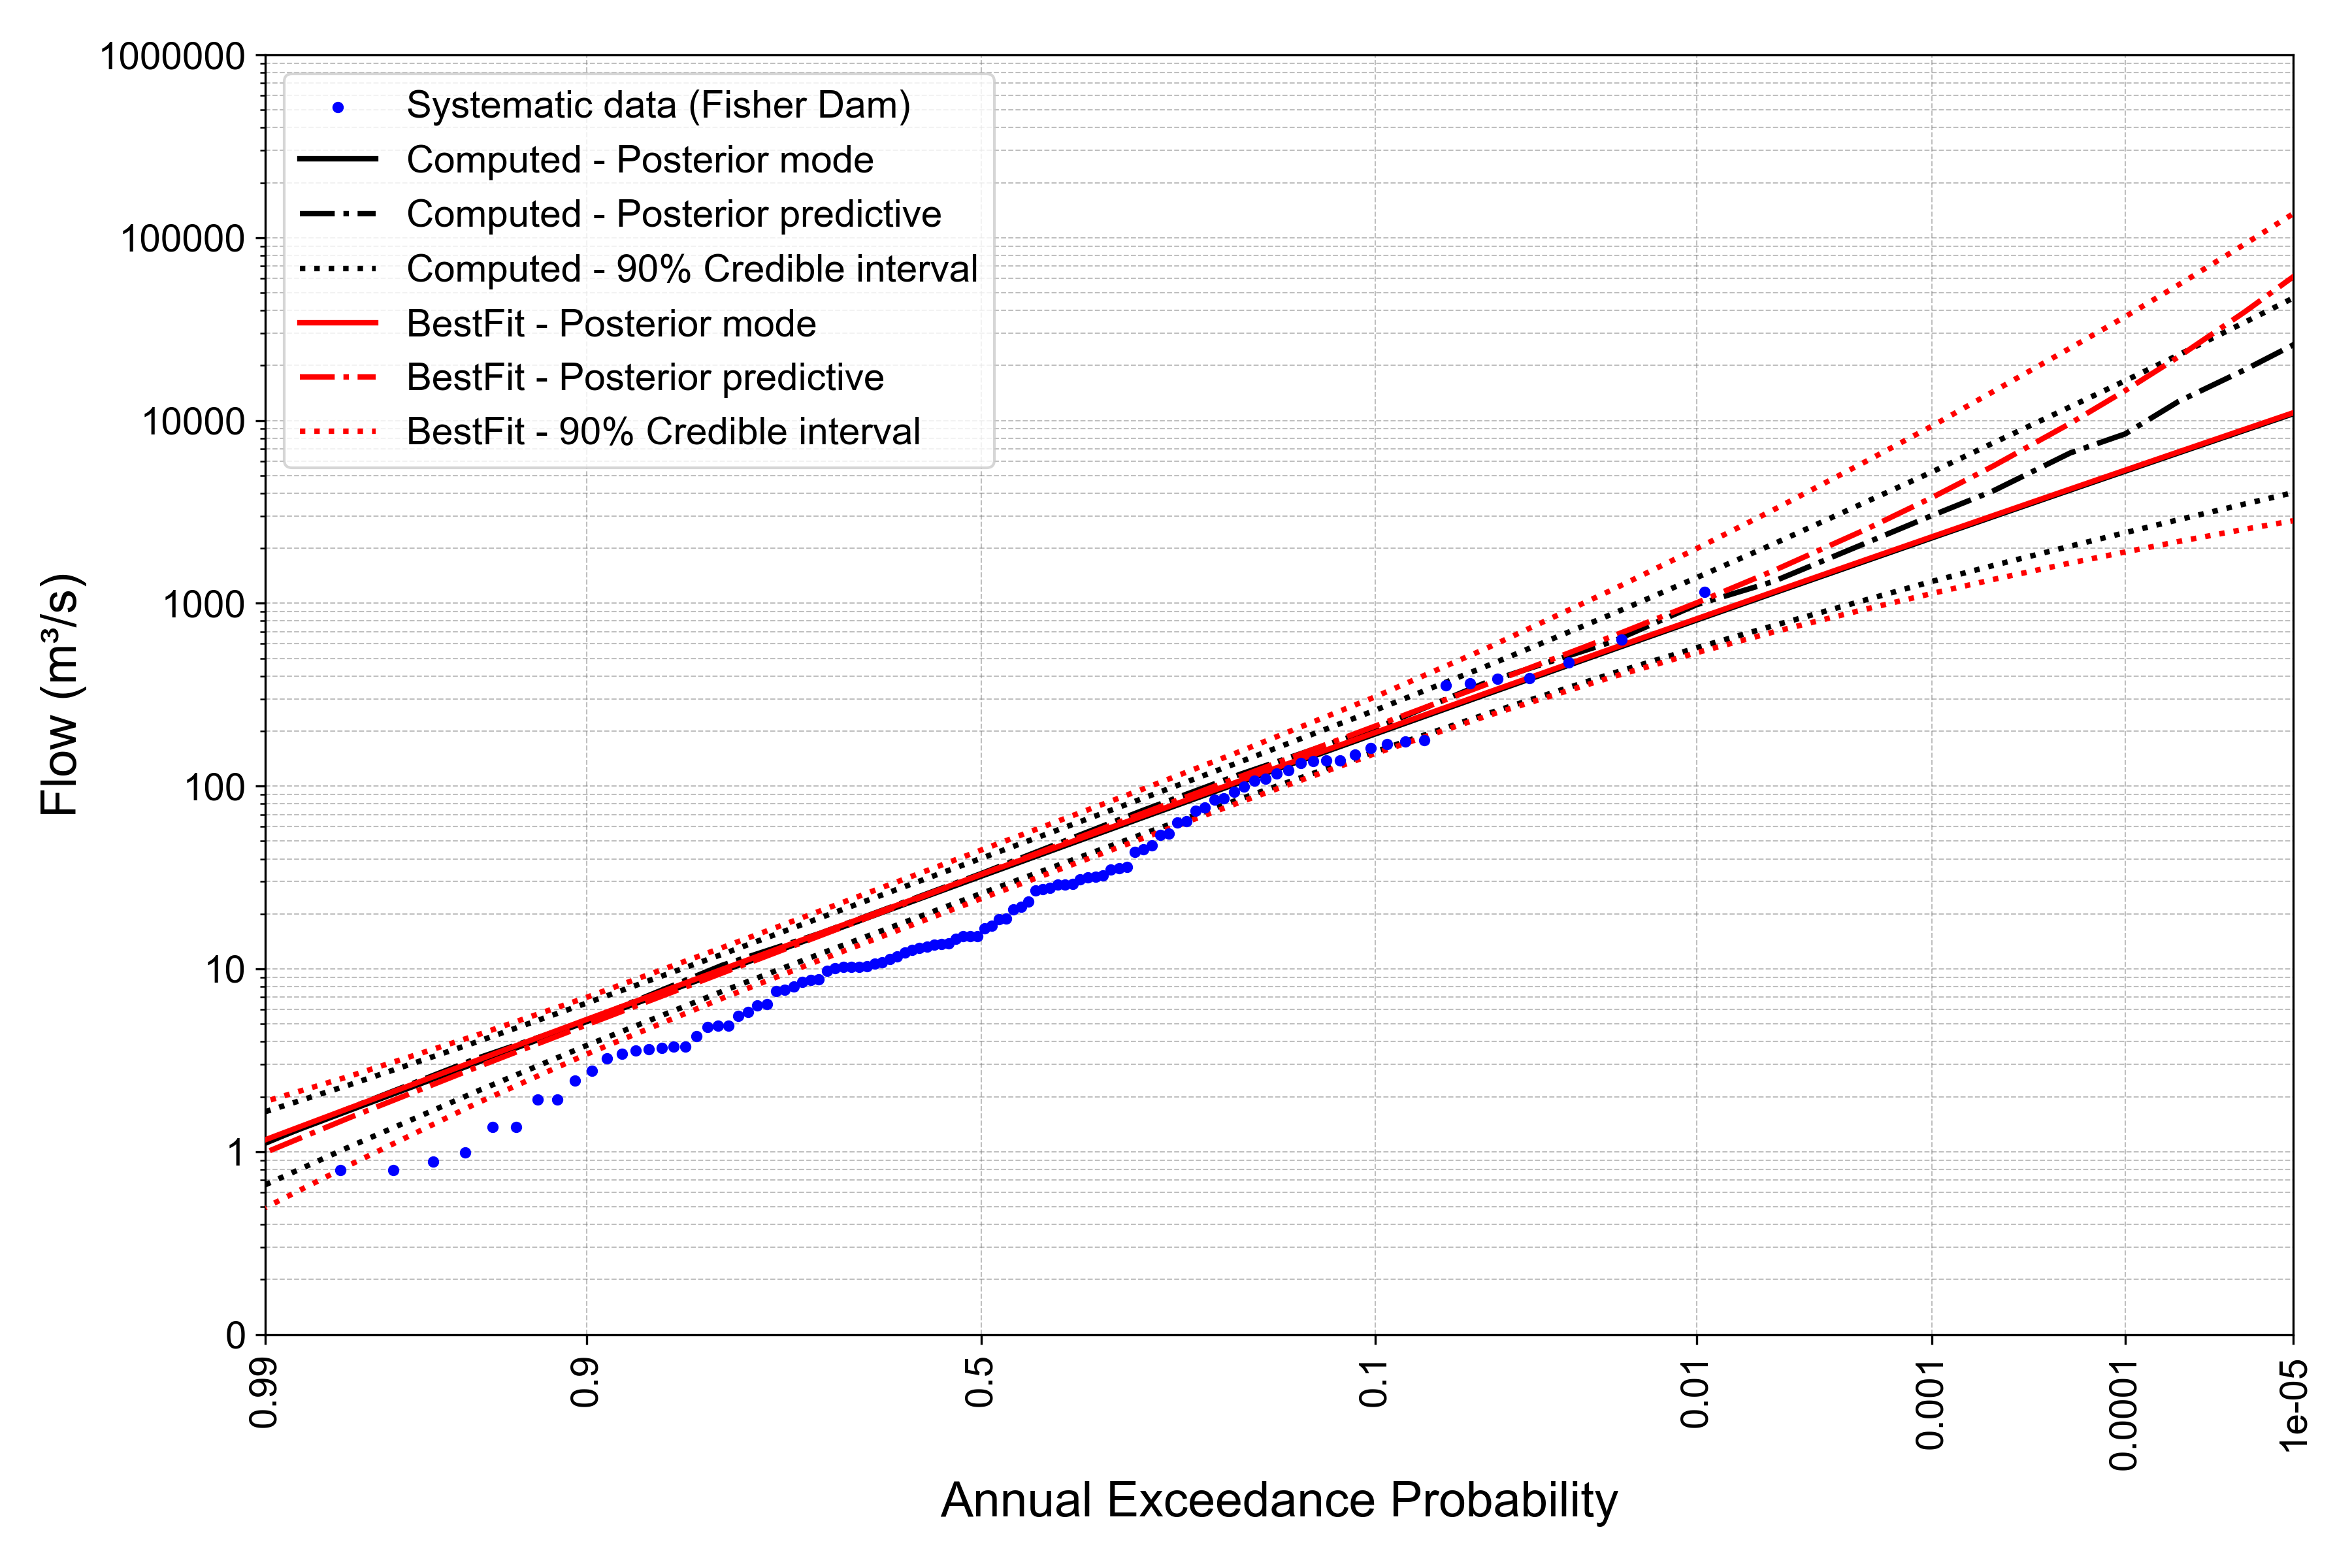
\includegraphics[width=1\linewidth]{_plots/OCD_bayesian_flood_quantiles_lp3_linear_mu.png}
    \caption{Comparison of computed Bayesian flood frequency curves with BestFit for the Fisher Dam NSFFA model with linear trend.}
    \label{fig:OCD_bayesian_flood_quantiles_lp3_linear_mu}
\end{figure*}

\begin{figure*}[htp]
    \centering
    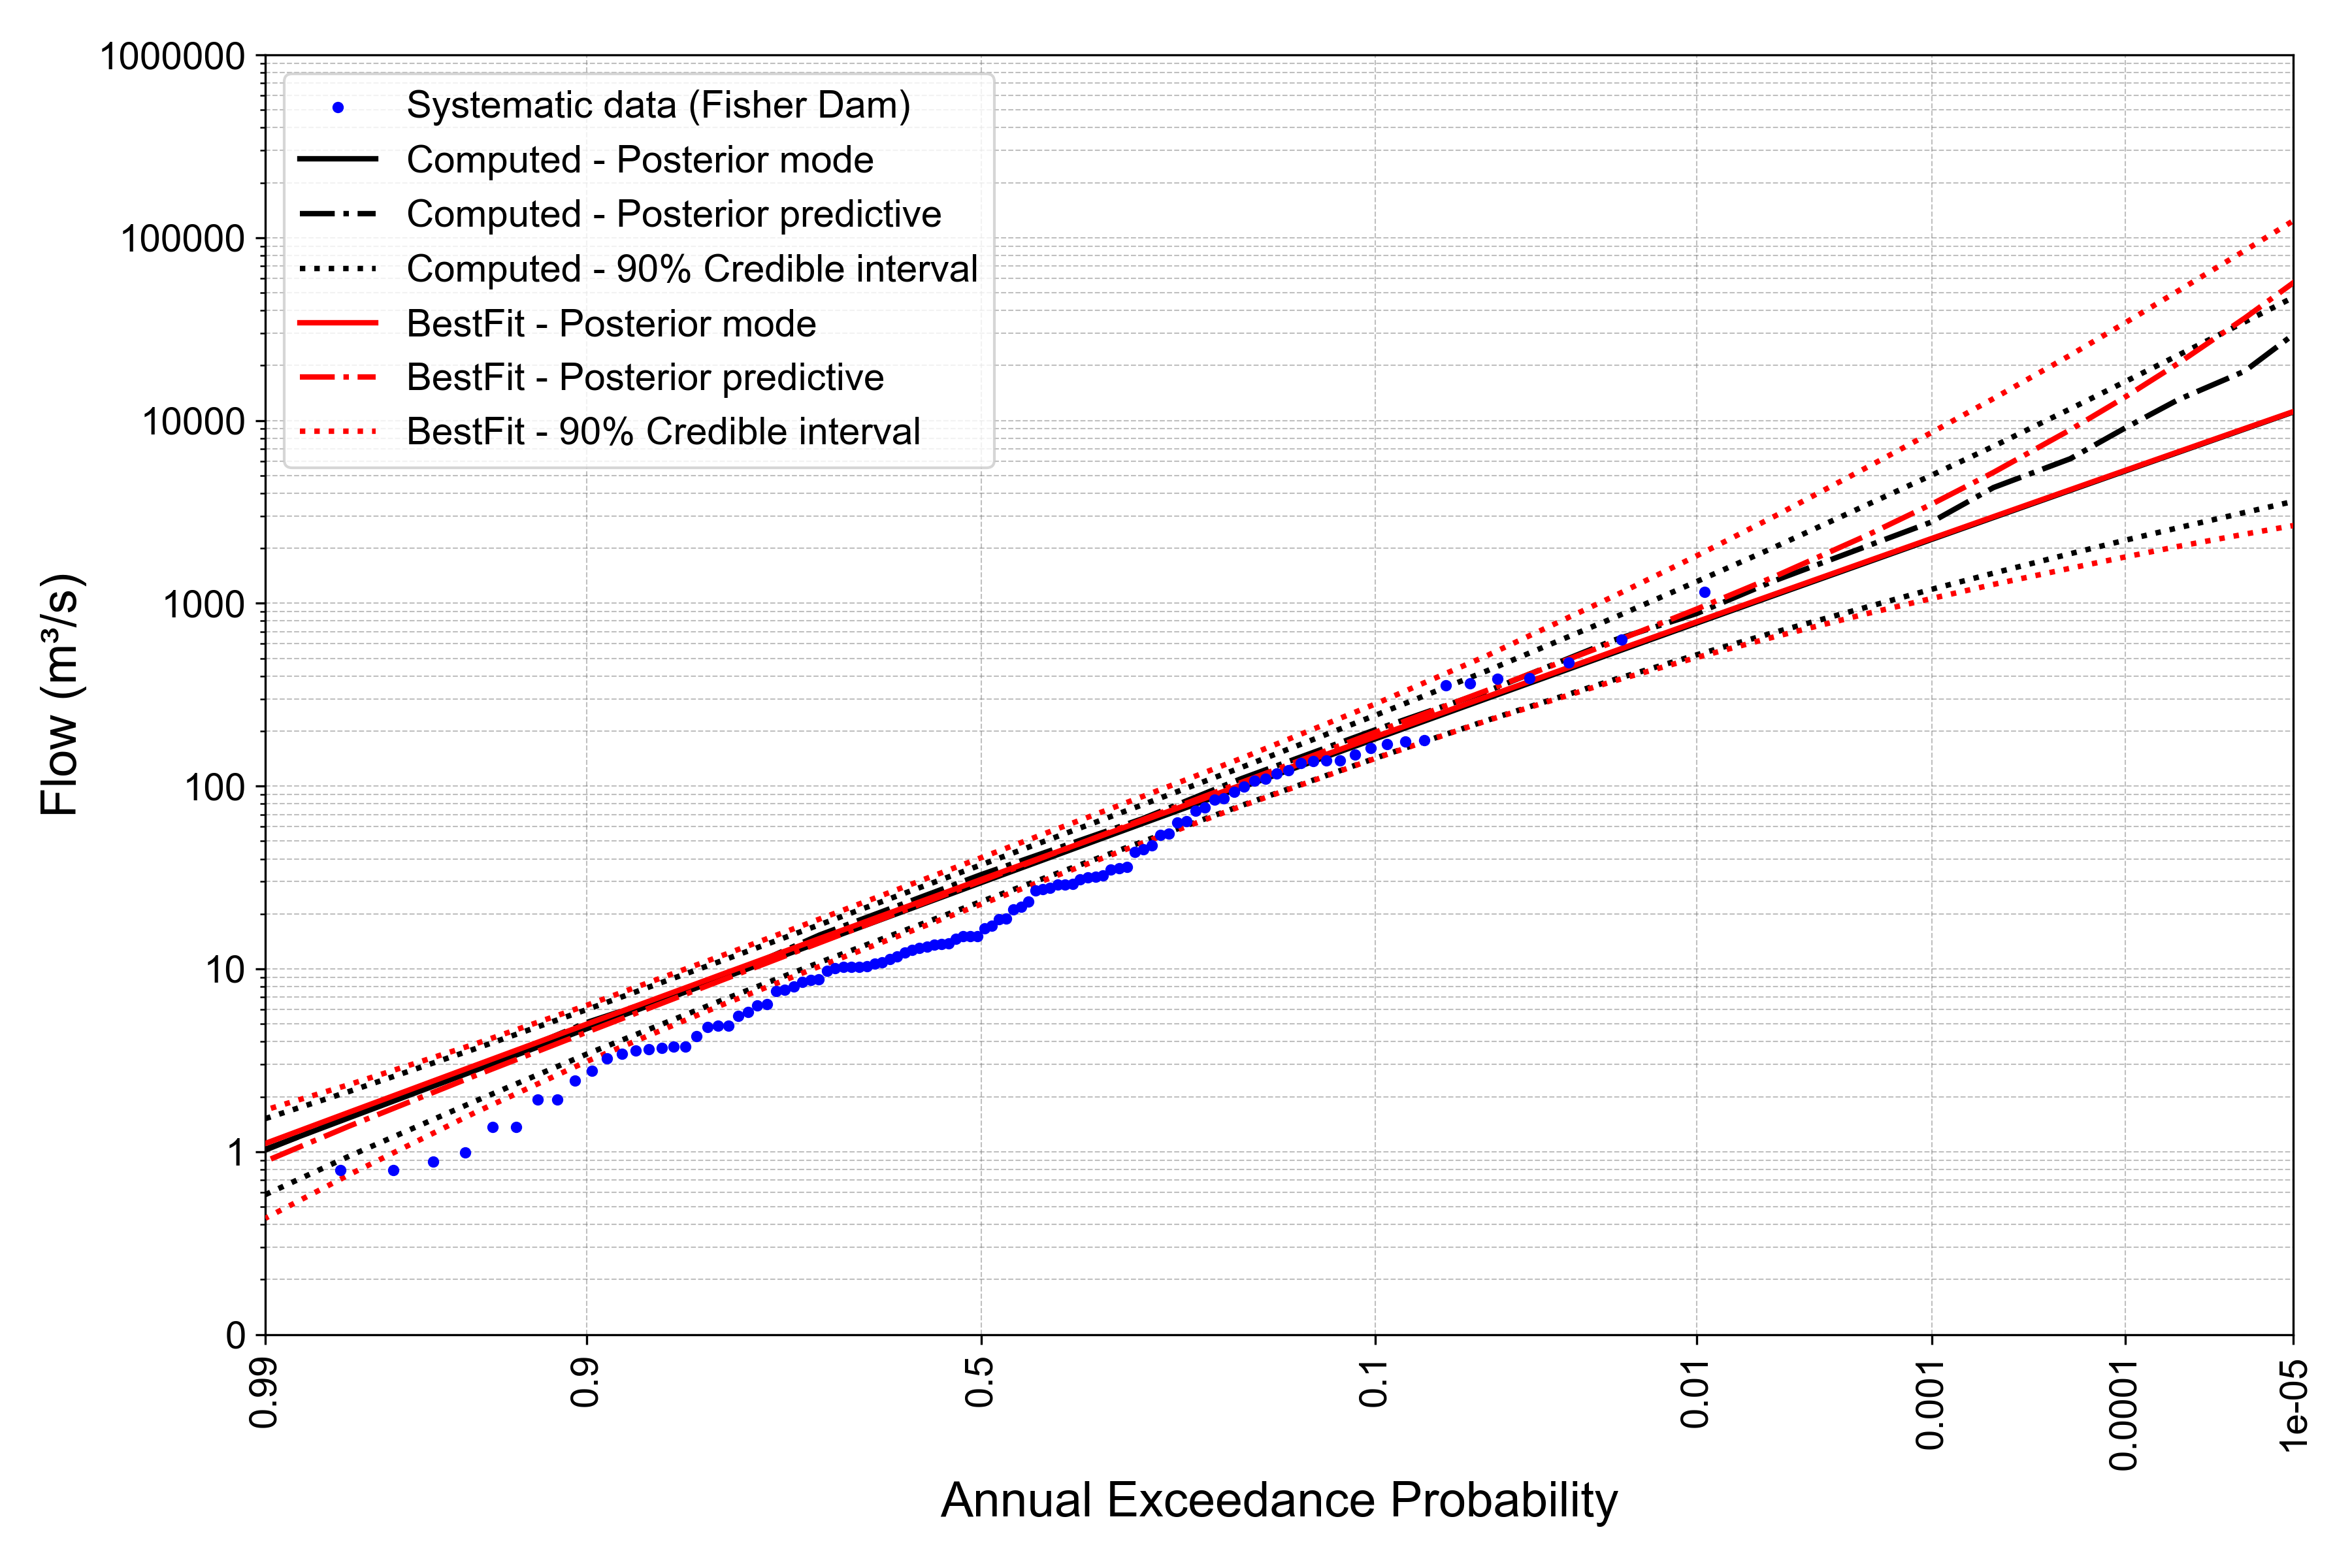
\includegraphics[width=1\linewidth]{_plots/OCD_bayesian_flood_quantiles_lp3_exponential_mu.png}
    \caption{Comparison of computed Bayesian flood frequency curves with BestFit for the Fisher Dam NSFFA model with exponential trend. }
\label{fig:OCD_bayesian_flood_quantiles_lp3_exponential_mu}
\end{figure*}

\FloatBarrier

\end{document}